\documentclass[11pt, b4paper, twoside]{scrartcl}
\nonstopmode
\usepackage[utf8]{inputenc}
\usepackage{tikz}
\usepackage{tikz-feynman}
\usepackage{caption}
\usepackage{subcaption}
\usepackage{dsfont}
\usepackage{enumitem}
\usepackage{bigints}
\allowdisplaybreaks
\usepackage{setspace}
\usepackage[T1]{fontenc}
\usepackage{babel}
\usepackage{graphicx} % Required for including pictures
\usepackage{fancyhdr}
\pagestyle{fancy}
\fancyhead{}
\fancyhead[RE]{ICTP | Assignment \#1}
\fancyhead[LE]{\thepage}
\usepackage{float}
\usepackage{mathpazo}
\usepackage{xcolor}
\definecolor{alizarin}{rgb}{0.82, 0.1, 0.26}
\usepackage[colorlinks = true,
            linkcolor = alizarin,
            urlcolor  = alizarin,
            citecolor = alizarin,
            anchorcolor = blue]{hyperref}
\usepackage[left=1in, top=1in, right=1in, bottom=0.8in]{geometry}
\usepackage[figurename=Figure]{caption}
\usepackage{float}    % For tables and other floats
\usepackage{verbatim} % For comments and other
\usepackage{amsmath}  % For math
\usepackage{amssymb}  % For more math
\usepackage{fullpage} % Set margins and place page numbers at bottom center
\usepackage{paralist} % paragraph spacing
\usepackage{listings} % For source code
\usepackage{subfig}   % For subfigures
%\usepackage{physics}  % for simplified dv, and 
\usepackage{enumitem} % useful for itemization
\usepackage{siunitx}  % standardization of si units

\usepackage{tikz,bm} % Useful for drawing plots
%\usepackage{tikz-3dplot}
\usepackage{circuitikz}

%%% Colours used in field vectors and propagation direction
\definecolor{mycolor}{rgb}{1,0.2,0.3}
\definecolor{brightgreen}{rgb}{0.4, 1.0, 0.0}
\definecolor{britishracinggreen}{rgb}{0.0, 0.26, 0.15}
\definecolor{cadmiumgreen}{rgb}{0.0, 0.42, 0.24}
\definecolor{ceruleanblue}{rgb}{0.16, 0.32, 0.75}
\definecolor{darkelectricblue}{rgb}{0.33, 0.41, 0.47}
\definecolor{darkpowderblue}{rgb}{0.0, 0.2, 0.6}
\definecolor{darktangerine}{rgb}{1.0, 0.66, 0.07}
\definecolor{emerald}{rgb}{0.31, 0.78, 0.47}
\definecolor{palatinatepurple}{rgb}{0.41, 0.16, 0.38}
\definecolor{pastelviolet}{rgb}{0.8, 0.6, 0.79}
\onehalfspacing
\linespread{1.25}
\usepackage{centernot}
\usepackage{slashed}
\newcommand{\fsl}[1]{{\centernot{#1}}}
\begin{document}
%---------------------
% \allowdisplaybreaks
\begin{center}
	\hrule
	\vspace{.4cm}
 \begin{tabular*}{\textwidth}{@{}l@{}|@{\extracolsep{0.6in}}r@{}}%
\parbox{4.25in}{\raggedright{
\includegraphics[width=.9\linewidth]{ictp-pwf.pdf}}} &
\parbox[c][]{4in}{{\Large\textbf{Md Akiful Islam Zawad} \par}
                    { Brac University \par}
                    { KHA 224, Progati Sarani, Merul Badda, \par}
                    { Dhaka 1212, Bangladesh \par}
                    { \href{ext.akiful.islam@bracu.ac.bd}{ext.akiful.islam@bracu.ac.bd}} \par}
\end{tabular*}\vspace{.3in}
\definecolor{ceruleanblue}{rgb}{0.16, 0.32, 0.6}
	\LARGE\scshape\textbf{\textcolor{ceruleanblue}{Physics For Bangladesh: School On Quantum Field Theory}}
\end{center}
\hrule\vspace{.25in}
{\large\textbf{Problem Sheet:}\ \textsc{1} \hspace{\hfill} \large\textbf{Submission Date:} \today\\
	\hline\hline
 %----------------------------
\paragraph*{Problem Set 1} %\hfill \newline
\\
A Lorentz transformation $x^\mu \rightarrow x'^\mu = \Lambda^\mu_\nu x^\nu$ is such that $\eta_{\mu\nu} x^\mu x^\nu = \eta_{\mu\nu} x'^\mu x'^\nu$ where $\eta_{\mu\nu}$ is the Minkowski metric and $x^\mu$ is any 4-vector.

    Show that this implies that
    \begin{align*}
        \eta_{\mu\nu} &= \eta_{\sigma\tau} \Lambda^\sigma_\mu \Lambda^\tau_\nu.
    \end{align*}
    Use this result to show that an infinitesimal transformation around identity of the form
    \begin{align*}
        \Lambda^\mu_\nu &= \delta^\mu_\nu + \omega^\mu_\nu,
    \end{align*}
    ($\omega^\mu_\nu$ is infinitesimally small) is a Lorentz transformation when $\omega_{\mu\nu}$ is antisymmetric: i.e. $\omega_{\mu\nu} = -\omega_{\nu\mu}$.
    
\bigskip\bigskip\hline\hline\bigskip

\section*{Solution}
We start with the given condition that the Minkowski metric is preserved under the Lorentz transformation:
\begin{align}
    \eta_{\mu\nu} x^\mu x^\nu &= \eta_{\mu\nu} x'^\mu x'^\nu.\label{eq:minkowski-metric-conserved}
\end{align}
Substitute the transformed coordinates \(x'^\mu = \Lambda^\mu_\sigma x^\sigma\) into the right-hand side of (\ref{eq:minkowski-metric-conserved}):
\begin{align}
    \eta_{\mu\nu} x^\mu x^\nu &= \eta_{\mu\nu} \Lambda^\mu_\sigma x^\sigma \Lambda^\nu_\tau x^\tau\notag\\
    &= \eta_{\sigma\tau} \Lambda^\sigma_\mu \Lambda^\tau_\nu x^\mu x^\nu.
\end{align}
Since this must hold for any 4-vector \(x^\mu\), we conclude that:
\begin{align}
    \eta_{\mu\nu} &= \eta_{\sigma\tau} \Lambda^\sigma_\mu \Lambda^\tau_\nu,\label{eq:desired-result}
\end{align}
which is the desired result.

Consider an infinitesimal Lorentz transformation of the form:
\begin{align}
    \Lambda^\mu_\nu &= \delta^\mu_\nu + \omega^\mu_\nu,\label{eq:infinitesimal-lorentz}
\end{align}
where \(\omega^\mu_\nu\) is infinitesimally small.

Substitute this into (\ref{eq:minkowski-metric-conserved}):
\begin{align*}
    \eta_{\mu\nu} &= \eta_{\sigma\tau} \Lambda^\sigma_\mu \Lambda^\tau_\nu.\label{eq:minkowski-metric-conserved-2}
\end{align*}
Expanding \(\Lambda^\sigma_\mu \Lambda^\tau_\nu\) to first order in \(\omega\), we get:
\begin{align}
    \Lambda^\sigma_\mu \Lambda^\tau_\nu &= (\delta^\sigma_\mu + \omega^\sigma_\mu)(\delta^\tau_\nu + \omega^\tau_\nu) \notag \\
    &= \delta^\sigma_\mu \delta^\tau_\nu + \delta^\sigma_\mu \omega^\tau_\nu + \omega^\sigma_\mu \delta^\tau_\nu + \mathcal{O}(\omega^2)\notag\\
    &= \delta^\sigma_\mu \delta^\tau_\nu + \omega^\tau_\nu \delta^\sigma_\mu + \omega^\sigma_\mu \delta^\tau_\nu + \mathcal{O}(\omega^2).
\end{align}
Substitute this into (\ref{eq:minkowski-metric-conserved-2}):
\begin{align}
    \eta_{\mu\nu} &= \eta_{\sigma\tau} \left(\delta^\sigma_\mu \delta^\tau_\nu + \omega^\tau_\nu \delta^\sigma_\mu + \omega^\sigma_\mu \delta^\tau_\nu \right)\notag\\
    &= \eta_{\sigma\tau} \delta^\sigma_\mu \delta^\tau_\nu + \eta_{\sigma\tau} \delta^\sigma_\mu \omega^\tau_\nu + \eta_{\sigma\tau} \omega^\sigma_\mu \delta^\tau_\nu\notag\\
    &= \eta_{\mu\nu} + \eta_{\mu\tau} \omega^\tau_\nu + \eta_{\sigma\nu} \omega^\sigma_\mu\notag\\
    0 &= \eta_{\mu\tau} \omega^\tau_\nu + \eta_{\sigma\nu} \omega^\sigma_\mu.
\end{align}
Since \(\eta_{\mu\tau}\) is the Minkowski metric and is symmetric, this equation implies that:
\begin{align}
    \omega_{\mu\nu} &= -\omega_{\nu\mu},
\end{align}
which shows that \(\omega_{\mu\nu}\) must be antisymmetric.
% \allowdisplaybreaks
\begin{center}
	\hrule
	\vspace{.4cm}
 \begin{tabular*}{\textwidth}{@{}l@{}|@{\extracolsep{0.6in}}r@{}}%
\parbox{4.25in}{\raggedright{
\includegraphics[width=.9\linewidth]{ictp-pwf.pdf}}} &
\parbox[c][]{4in}{{\Large\textbf{Md Akiful Islam Zawad} \par}
                    { Brac University \par}
                    { KHA 224, Progati Sarani, Merul Badda, \par}
                    { Dhaka 1212, Bangladesh \par}
                    { \href{ext.akiful.islam@bracu.ac.bd}{ext.akiful.islam@bracu.ac.bd}} \par}
\end{tabular*}\vspace{.3in}
\definecolor{ceruleanblue}{rgb}{0.16, 0.32, 0.6}
	\LARGE\scshape\textbf{\textcolor{ceruleanblue}{Physics For Bangladesh: School On Quantum Field Theory}}
\end{center}
\hrule\vspace{.25in}
{\large\textbf{Problem Sheet:}\ \textsc{1} \hspace{\hfill} \large\textbf{Submission Date:} \today\\
	\hline\hline
 %----------------------------
\paragraph*{Problem Set 2} %\hfill \newline
\\
The Lagrangian density for a complex scalar field $\displaystyle\Phi(x) = \phi_1(x) + i\phi_2(x)$ is given by
    \begin{align*}
        \mathcal{L} = \partial_\mu \Phi^* \partial^\mu \Phi - m^2 \Phi^* \Phi - \frac{\lambda}{2} (\Phi^* \Phi)^2.
    \end{align*}
    \begin{enumerate}
        \item Write down the Euler-Lagrange equations of motion (EOM). Verify that the Lagrangian is invariant under the infinitesimal transformations
    \begin{align*}
        \delta \Phi = i\alpha \Phi, \quad \delta \Phi^* = -i\alpha \Phi^*
    \end{align*}
    which is an infinitesimal version of $\displaystyle\Phi \rightarrow e^{i\alpha} \Phi$.
    \item Derive the Noether current associated with this transformation and verify explicitly that it is conserved using the field equations satisfied by $\phi$.
    \item It is also instructive to write $\mathcal{L}$ in terms of the two real scalar fields $\phi_1, \phi_2$. Can you justify the numerical factors that appeared in the Lagrangian?
    \end{enumerate}
\bigskip\bigskip\hline\hline\bigskip
\section*{Solution}
\subsection*{\scshape\bf 1. Invariance of Lagrangian}
The Lagrangian density for a complex scalar field $\Phi(x)$ is given by
\begin{align}
    \mathcal{L} &= \partial_\mu \Phi^* \partial^\mu \Phi - m^2 \Phi^* \Phi - \frac{\lambda}{2} (\Phi^* \Phi)^2. \label{eq:lagrangian-density-complex-scalar}
\end{align}
The Euler-Lagrange equation for a field $\Phi(x)$ is given by:
\begin{align}
    \frac{\partial \mathcal{L}}{\partial \Phi} - \partial_\mu \left( \frac{\partial \mathcal{L}}{\partial (\partial_\mu \Phi)} \right) &= 0.\label{eq:euler-lagrange-for-fields}
\end{align}
Let's first compute each term:

Partial derivative of $\mathcal{L}$ with respect to $\Phi$:
  \begin{align*}
      \frac{\partial \mathcal{L}}{\partial \Phi} &= - m^2 \Phi^* - \lambda \Phi^* (\Phi^* \Phi).
  \end{align*}
Partial derivative of $\mathcal{L}$ with respect to $\partial_\mu \Phi$:
  \begin{align*}
      \frac{\partial \mathcal{L}}{\partial (\partial_\mu \Phi)} &= \partial^\mu \Phi^*.
  \end{align*}
Derivative with respect to $x^\mu$:
  \begin{align*}
      \partial_\mu \left( \frac{\partial \mathcal{L}}{\partial (\partial_\mu \Phi)} \right) &= \partial_\mu \partial^\mu \Phi^*.
  \end{align*}
Now, substituting these into (\ref{eq:euler-lagrange-for-fields}):
\begin{align}
    - m^2 \Phi^* - \lambda \Phi^* (\Phi^* \Phi) - \partial_\mu \partial^\mu \Phi^* &= 0\notag\\
    \partial_\mu\partial^\mu \Phi^* + m^2 \Phi^* + \lambda \Phi^* (\Phi^* \Phi)\label{eq:conjugate-euler-lagrange}
\end{align}
Taking the complex conjugate of (\ref{eq:conjugate-euler-lagrange}) gives the equation of motion for $\Phi$:
\begin{align}
    \partial_\mu \partial^\mu \Phi + m^2 \Phi + \lambda (\Phi^* \Phi) \Phi &= 0. \label{eq:EOM}
\end{align}
We now need to verify that the Lagrangian is invariant under the infinitesimal transformations:
\begin{align*}
    \delta \Phi &= i\alpha \Phi, \quad \delta \Phi^* = -i\alpha \Phi^*,
\end{align*}
where $\alpha$ is an infinitesimally small constant.

The change in the Lagrangian $\delta \mathcal{L}$ (\ref{eq:lagrangian-density-complex-scalar}) under this transformation is given by:
\begin{align}
    \delta \mathcal{L} &= \frac{\partial \mathcal{L}}{\partial \Phi} \delta \Phi + \frac{\partial \mathcal{L}}{\partial \Phi^*} \delta \Phi^*.
\end{align}
Substitute the given transformations:
\begin{align}
    \delta \mathcal{L} &= \frac{\partial \mathcal{L}}{\partial \Phi} (i\alpha \Phi) + \frac{\partial \mathcal{L}}{\partial \Phi^*} (-i\alpha \Phi^*) \notag \\
    &= i\alpha \Phi \frac{\partial \mathcal{L}}{\partial \Phi} - i\alpha \Phi^* \frac{\partial \mathcal{L}}{\partial \Phi^*}\notag\\
    &= i\alpha \Phi \left[-m^2 \Phi^* - \lambda \Phi^* (\Phi^* \Phi)\right] - i\alpha \Phi^* \left[-m^2 \Phi - \lambda \Phi (\Phi^* \Phi)\right]\notag\\[6pt]
    &= 0,\notag
\end{align}
which shows that the Lagrangian is indeed invariant under the given transformations.
\subsection*{\scshape\bf 2. Noether Current}
Noether's theorem states that for every continuous symmetry of the action, there is a corresponding conserved current. The conserved current $J^\mu$ associated with the symmetry is given by:
\begin{align}
    J^\mu &= \frac{\partial \mathcal{L}}{\partial (\partial_\mu \Phi)} \delta \Phi + \frac{\partial \mathcal{L}}{\partial (\partial_\mu \Phi^*)} \delta \Phi^*.\label{eq:noether-current}\notag\\
    &= \partial^\mu \Phi^* (i\alpha \Phi) + \partial^\mu \Phi (-i\alpha \Phi^*) \notag \\[6pt]
    &= i\alpha (\Phi \partial^\mu \Phi^* - \Phi^* \partial^\mu \Phi).
\end{align}
Thus, the Noether current is:
\begin{align}
    J^\mu &= \alpha (\Phi \partial^\mu \Phi^* - \Phi^* \partial^\mu \Phi). \label{eq:Noether-Current}
\end{align}
To verify that this current is conserved, we compute its divergence:
\begin{align}
    \partial_\mu J^\mu &= \alpha \partial_\mu (\Phi \partial^\mu \Phi^* - \Phi^* \partial^\mu \Phi).\label{eq:noether-current-divergence}
\end{align}
Using the equations of motion (EOM) (\ref{eq:EOM}):
\begin{align*}
    \partial_\mu \partial^\mu \Phi &= -m^2 \Phi - \lambda (\Phi^* \Phi) \Phi, \notag \\
    \partial_\mu \partial^\mu \Phi^* &= -m^2 \Phi^* - \lambda (\Phi^* \Phi) \Phi^*,
\end{align*}
we can see that:
\begin{align}
    \partial_\mu J^\mu &= 0,
\end{align}
confirming that $J^\mu$ is indeed conserved.
\subsection*{\scshape\bf 3. Lagrangian in Terms of Real Scalar Fields}
We can express the complex scalar field $\Phi(x)$ in terms of two real scalar fields $\phi_1(x)$ and $\phi_2(x)$ as:
\begin{align*}
    \Phi(x) &= \phi_1(x) + i \phi_2(x), \\
    \Phi^*(x) &= \phi_1(x) - i \phi_2(x).
\end{align*}
Substituting into the Lagrangian (\ref{eq:lagrangian-density-complex-scalar}):
\begin{align*}
    \mathcal{L} &= \partial_\mu (\phi_1 - i\phi_2) \partial^\mu (\phi_1 + i\phi_2) - m^2 (\phi_1^2 + \phi_2^2) - \frac{\lambda}{2} (\phi_1^2 + \phi_2^2)^2\notag\\
    &= (\partial_\mu \phi_1 \partial^\mu \phi_1 + \partial_\mu \phi_2 \partial^\mu \phi_2) - m^2 (\phi_1^2 + \phi_2^2) - \frac{\lambda}{2} (\phi_1^2 + \phi_2^2)^2.
\end{align*}
This is the Lagrangian density expressed in terms of the real scalar fields $\phi_1(x)$ and $\phi_2(x)$. The numerical factors appear due to the standard normalization and the structure of the interaction terms.
% \allowdisplaybreaks
\begin{center}
	\hrule
	\vspace{.4cm}
 \begin{tabular*}{\textwidth}{@{}l@{}|@{\extracolsep{0.6in}}r@{}}%
\parbox{4.25in}{\raggedright{
\includegraphics[width=.9\linewidth]{ictp-pwf.pdf}}} &
\parbox[c][]{4in}{{\Large\textbf{Md Akiful Islam Zawad} \par}
                    { Brac University \par}
                    { KHA 224, Progati Sarani, Merul Badda, \par}
                    { Dhaka 1212, Bangladesh \par}
                    { \href{ext.akiful.islam@bracu.ac.bd}{ext.akiful.islam@bracu.ac.bd}} \par}
\end{tabular*}\vspace{.3in}
\definecolor{ceruleanblue}{rgb}{0.16, 0.32, 0.6}
	\LARGE\scshape\textbf{\textcolor{ceruleanblue}{Physics For Bangladesh: School On Quantum Field Theory}}
\end{center}
\hrule\vspace{.25in}
{\large\textbf{Problem Sheet:}\ \textsc{1} \hspace{\hfill} \large\textbf{Submission Date:} \today\\
	\hline\hline
 %----------------------------
\paragraph*{Problem Set 3} %\hfill \newline
\\
Verify Wick's theorem for
    \begin{enumerate}
        \item The product of three scalars:
        \begin{align*}
            T(\phi(x_1) \phi(x_2) \phi(x_3)) = : \phi(x_1) \phi(x_2) \phi(x_3) : + \phi(x_1) \Delta_F(x_2 - x_3)
        + \phi(x_2) \Delta_F(x_3 - x_1) + \phi(x_3) \Delta_F(x_1 - x_2)
        \end{align*}
        \item The product of four scalars:
        \begin{align*}
            T(\phi(x_1) \phi(x_2) \phi(x_3) \phi(x_4))    
        \end{align*}
    \end{enumerate}

\bigskip\bigskip\hline\hline\bigskip
\section*{Solution}
Wick's theorem states that the time-ordered product of a set of fields can be expressed as a sum of normal-ordered products with contractions. For scalar fields, the contraction between two fields is defined as the Feynman propagator $\Delta_F(x - y)$.

Wick’s Theorem states that for $n$ field operators, the time-ordered product can be written as a sum over all possible ways of contracting the operators. 

For two scalar fields $\phi(x_1)\equiv\phi_1$ and $\phi(x_2)\equiv\phi_2$, the theorem is:

\begin{align}
    T \{\phi_1\phi_2\} &= :\phi_1\phi_2: + \overbrace{\phi_1,\phi_2}
\end{align}
The time-ordered product of two scalar field is defined as
\begin{align*}
    T \{\phi_1\phi_2\} &= \begin{cases}
      \phi_1\phi_2; & x_1^0 > x_2^0\\
      \phi_2\phi_1; & x_2^0 > x_1^0
    \end{cases}
\end{align*}
or \begin{align*}
    T \{\phi_1\phi_2\}=\theta\left(x_1^0-x_2^0\right)\phi_1\phi_2+\theta\left(x_2^0-x_1^0\right)\phi_2\phi_1,
\end{align*}
from which it is clear that $T \{\phi_1\phi_2\}$ is symmetric in $x_1$ and $x_2$.

The normal-ordered product of two fields is defined as
\begin{align*}
    :\phi_1\phi_2:=:\left(\phi_1^++\phi_1^-\right)+\left(\phi_2^-+\phi_2^-\right):=\phi_1^+\phi_2^++\phi_2^-\phi_1^++\phi_1^-\phi_2^++\phi_1^-\phi_2^-
\end{align*}
The Feynmann propagator may be written as
\begin{align}
    \Delta_F\left(x_1-x_2\right)=T\{\phi_1\phi_2\}-:\phi_1\phi_2:
\end{align}
We now attempt to check Wick's theorem fir the time-ordered product of three scalar fields. First, consider the case, $x_1^0>x_2^0>x_3^0$:
\begin{align}
    T\left\{\phi_1\phi_2\phi_3\right\}&=\phi_1\phi_2\phi_3=\left(\phi_1^++\phi_1^-\right)\left(\phi_2^++\phi_2^-\right)\left(\phi_3^++\phi_3^-\right)\notag\\
    &=\phi_1^+\phi_2^+\phi_3^++\phi_1^+\phi_2^+\phi_3^-+\phi_1^+\phi_2^-\phi_3^++\phi_1^+\phi_2^-\phi_3^-+\phi_1^-\phi_2^+\phi_3^++\phi_1^-\phi_2^+\phi_3^-+\phi_1^-\phi_2^-\phi_3^++\phi_1^-\phi_2^-\phi_3^-\notag\\
    &=\phi_1^+\phi_2^+\phi_3^+\left(\phi_3^-\phi_1^+\phi_2^++\left[\phi_1^+,\phi_3^-\right]\phi_2^++\phi_1^+\left[\phi_2^+,\phi_3^-\right]\right)+\left(\phi_2^-\phi_2^+\phi_3^++\left[\phi_1^+,\phi_2^-\right]\phi_3^+\right)\notag\\
    &\hspace{20pt}\left(\phi_2^-\phi_3^-\phi_1^++\phi_2^-\left[\phi_1^+,\phi_3^-\right]+\left[\phi_1^+,\phi_2^-\right]\phi_3^-\right)+\phi_1^-\phi_2^+\phi_3^+\notag\\
    &\hspace{40pt}\left(\phi_1^-\phi_2^+\phi_3^-+\phi_1^-\left[\phi_1^+,\phi_3^-\right]\right)+\phi_1^-\phi_3^+\phi_2^-+\phi_1^-\phi_2^-\phi_3^-\notag\\
    &=:\phi_1\phi_2\phi_3:+\left[\phi_1^+,\phi_3^-\right]\phi_2+\left[\phi_2^+,\phi_3^-\right]\phi_1+\left[\phi_1^+,\phi_3^-\right]\phi_3\notag\\
    &=:\phi_1\phi_2\phi_3:+\Delta_F\left(x_1-x_3\right)\phi_2+\Delta_F\left(x_2-x_3\right)\phi_1+\Delta_F\left(x_1-x_2\right)\phi_3\notag
\end{align}
As a re-ordering of $x_1^0>x_2^0>x_3^0$ corresponds to a different choice of labels and since $\Delta_F$ and normal ordered products are symmetric, this calculation suffices to prove Wick’s theorem.

Thus, Wick's theorem is verified for the product of three scalar fields.

Now, we verify Wick's theorem for the product of four scalar fields:
\begin{align}
    T\left\{\phi_1 \phi_2 \phi_3 \phi_4\right\} &= \left(\phi_1^+ + \phi_1^-\right)\left(\phi_2^+ + \phi_2^-\right)\left(\phi_3^+ + \phi_3^-\right)\left(\phi_4^+ + \phi_4^-\right) \notag \\
    &= \phi_1^+ \phi_2^+ \phi_3^+ \phi_4^+ + \phi_1^+ \phi_2^+ \phi_3^+ \phi_4^- + \phi_1^+ \phi_2^+ \phi_3^- \phi_4^+ + \phi_1^+ \phi_2^+ \phi_3^- \phi_4^- \notag \\
    &\quad + \phi_1^+ \phi_2^- \phi_3^+ \phi_4^+ + \phi_1^+ \phi_2^- \phi_3^+ \phi_4^- + \phi_1^+ \phi_2^- \phi_3^- \phi_4^+ + \phi_1^+ \phi_2^- \phi_3^- \phi_4^- \notag \\
    &\quad + \phi_1^- \phi_2^+ \phi_3^+ \phi_4^+ + \phi_1^- \phi_2^+ \phi_3^+ \phi_4^- + \phi_1^- \phi_2^+ \phi_3^- \phi_4^+ + \phi_1^- \phi_2^+ \phi_3^- \phi_4^- \notag \\
    &\quad + \phi_1^- \phi_2^- \phi_3^+ \phi_4^+ + \phi_1^- \phi_2^- \phi_3^+ \phi_4^- + \phi_1^- \phi_2^- \phi_3^- \phi_4^+ + \phi_1^- \phi_2^- \phi_3^- \phi_4^- \notag \\
    &= :\phi_1 \phi_2 \phi_3 \phi_4: \notag \\
    &\quad + \left(\phi_1^+ \phi_2^+ \left[\phi_3^-, \phi_4^+\right] + \phi_1^+ \left[\phi_2^+, \phi_4^-\right] \phi_3^+ + \left[\phi_1^+, \phi_3^-\right] \phi_2^+ \phi_4^+ \right) \notag \\
    &\quad + \left(\phi_2^+ \phi_3^+ \left[\phi_1^-, \phi_4^+\right] + \phi_2^+ \left[\phi_1^+, \phi_4^-\right] \phi_3^+ + \left[\phi_2^+, \phi_3^-\right] \phi_1^+ \phi_4^+ \right) \notag \\
    &\quad + \left(\phi_3^+ \phi_4^+ \left[\phi_1^-, \phi_2^+\right] + \phi_3^+ \left[\phi_1^+, \phi_2^-\right] \phi_4^+ + \left[\phi_1^+, \phi_4^-\right] \phi_2^+ \phi_3^+ \right) \notag \\
    &\quad + \left(\phi_1^- \phi_2^- \left[\phi_3^+, \phi_4^-\right] + \phi_1^- \left[\phi_2^-, \phi_4^+\right] \phi_3^- + \left[\phi_1^-, \phi_3^+\right] \phi_2^- \phi_4^- \right) \notag \\
    &\quad + \left(\phi_2^- \phi_3^- \left[\phi_1^+, \phi_4^-\right] + \phi_2^- \left[\phi_1^-, \phi_4^+\right] \phi_3^- + \left[\phi_2^-, \phi_3^+\right] \phi_1^- \phi_4^- \right) \notag \\
    &\quad + \left(\phi_3^- \phi_4^- \left[\phi_1^+, \phi_2^-\right] + \phi_3^- \left[\phi_1^-, \phi_2^+\right] \phi_4^- + \left[\phi_1^-, \phi_4^+\right] \phi_2^- \phi_3^- \right)
\end{align}
We now attempt to check Wick's theorem for the time-ordered product of four scalar fields. First, consider the case, $x_1^0>x_2^0>x_3^0x^4>0$:

Start with the product:
\begin{align}
    \phi_1 \phi_2 \phi_3 \phi_4 &= \left(\phi_1^+ + \phi_1^-\right)\left(\phi_2^+ + \phi_2^-\right)\left(\phi_3^+ + \phi_3^-\right)\left(\phi_4^+ + \phi_4^-\right) \notag \\
    &= \phi_1^+ \phi_2^+ \phi_3^+ \phi_4^++ \phi_1^+ \phi_2^+ \phi_3^+ \phi_4^-+ \phi_1^+ \phi_2^+ \phi_3^- \phi_4^++ \phi_1^+ \phi_2^+ \phi_3^- \phi_4^- \notag \\
    &\quad + \phi_1^+ \phi_2^- \phi_3^+ \phi_4^++\phi_1^+ \phi_2^- \phi_3^+ \phi_4^-+ \phi_1^+ \phi_2^- \phi_3^- \phi_4^++ \phi_1^+ \phi_2^- \phi_3^- \phi_4^-+ \notag\\ &\quad +\phi_1^- \phi_2^+ \phi_3^+ \phi_4^++ \phi_1^- \phi_2^+ \phi_3^+ \phi_4^-+ \phi_1^- \phi_2^+ \phi_3^- \phi_4^++ \phi_1^- \phi_2^+ \phi_3^- \phi_4^- \notag \\
    &\quad + \phi_1^- \phi_2^- \phi_3^+ \phi_4^++ \phi_1^- \phi_2^- \phi_3^+ \phi_4^-+ \phi_1^- \phi_2^- \phi_3^- \phi_4^+ + \phi_1^- \phi_2^- \phi_3^- \phi_4^- \notag
\end{align}

% Now, apply the time-ordering operator \( T \) and use commutation relations to correct each term:

% \begin{align}
%     T\left\{\phi_1 \phi_2 \phi_3 \phi_4\right\} &= \phi_1^+ \phi_2^+ \phi_3^+ \phi_4^+ \notag \\
%     &\quad + T\left\{\phi_1^+ \phi_2^+ \phi_3^+ \phi_4^-\right\} \notag \\
%     &\quad + T\left\{\phi_1^+ \phi_2^+ \phi_3^- \phi_4^+\right\} \notag \\
%     &\quad + T\left\{\phi_1^+ \phi_2^+ \phi_3^- \phi_4^-\right\} \notag \\
%     &\quad + T\left\{\phi_1^+ \phi_2^- \phi_3^+ \phi_4^+\right\} \notag \\
%     &\quad + T\left\{\phi_1^+ \phi_2^- \phi_3^+ \phi_4^-\right\} \notag \\
%     &\quad + T\left\{\phi_1^+ \phi_2^- \phi_3^- \phi_4^+\right\} \notag \\
%     &\quad + T\left\{\phi_1^+ \phi_2^- \phi_3^- \phi_4^-\right\} \notag \\
%     &\quad + T\left\{\phi_1^- \phi_2^+ \phi_3^+ \phi_4^+\right\} \notag \\
%     &\quad + T\left\{\phi_1^- \phi_2^+ \phi_3^+ \phi_4^-\right\} \notag \\
%     &\quad + T\left\{\phi_1^- \phi_2^+ \phi_3^- \phi_4^+ \right\} \notag \\
%     &\quad + T\left\{\phi_1^- \phi_2^+ \phi_3^- \phi_4^- \right\} \notag \\
%     &\quad + T\left\{\phi_1^- \phi_2^- \phi_3^+ \phi_4^+ \right\} \notag \\
%     &\quad + T\left\{\phi_1^- \phi_2^- \phi_3^+ \phi_4^- \right\} \notag \\
%     &\quad + T\left\{\phi_1^- \phi_2^- \phi_3^- \phi_4^+ \right\} \notag \\
%     &\quad + T\left\{\phi_1^- \phi_2^- \phi_3^- \phi_4^- \right\} \notag
% \end{align}
Now expand and correct each time-ordered product term by term:
    \begin{align*}
        T\left\{\phi_1 \phi_2 \phi_3 \phi_4\right\} &= \phi_1^+ \phi_2^+ \phi_3^+ \phi_4^+\\[5pt]
        &\hspace{5pt}+\phi_1^+ \phi_2^+ \phi_3^+ \phi_4^-+ \left[\phi_4^-, \phi_1^+\right] \phi_2^+ \phi_3^++ \left[\phi_4^-, \phi_2^+\right] \phi_1^+ \phi_3^++ \left[\phi_4^-, \phi_3^+\right] \phi_1^+ \phi_2^+\\[5pt]
        &\hspace{10pt}+\phi_1^+ \phi_2^+ \phi_3^- \phi_4^++ \left[\phi_3^-, \phi_4^+\right] \phi_1^+ \phi_2^++ \left[\phi_1^+, \phi_3^- \right] \phi_2^+ \phi_4^++ \left[\phi_2^+, \phi_3^- \right] \phi_1^+ \phi_4^+\\[5pt]
        &\hspace{15pt}+\phi_1^+ \phi_2^+ \phi_3^- \phi_4^-+ \left[\phi_4^-, \phi_1^+\right] \phi_2^+ \phi_3^-+ \left[\phi_3^-, \phi_1^+\right] \phi_2^+ \phi_4^-+ \left[\phi_3^-, \phi_2^+\right] \phi_1^+ \phi_4^-\\[5pt]
        &\hspace{20pt}+\phi_1^+ \phi_2^- \phi_3^+ \phi_4^++ \left[\phi_2^-, \phi_3^+\right] \phi_1^+ \phi_4^++ \left[\phi_1^+, \phi_2^-\right] \phi_3^+ \phi_4^++ \left[\phi_1^+, \phi_4^+\right] \phi_2^- \phi_3^+\\[5pt]
        &\hspace{25pt}+\phi_1^+ \phi_2^- \phi_3^+ \phi_4^-+ \left[\phi_4^-, \phi_2^-\right] \phi_1^+ \phi_3^++ \left[\phi_3^+, \phi_2^-\right] \phi_1^+ \phi_4^-+ \left[\phi_1^+, \phi_2^-\right] \phi_3^+ \phi_4^-\\[5pt]
        &\hspace{30pt}+\phi_1^+ \phi_2^- \phi_3^- \phi_4^++\left[\phi_3^-, \phi_4^+\right] \phi_1^+ \phi_2^-+\left[\phi_2^-, \phi_4^+\right] \phi_1^+ \phi_3^-+\left[\phi_2^-, \phi_3^- \right] \phi_1^+ \phi_4^+\\[5pt]
        &\hspace{35pt}+\phi_1^+ \phi_2^- \phi_3^- \phi_4^-+\left[\phi_3^-, \phi_4^-\right] \phi_1^+ \phi_2^-+\left[\phi_2^-, \phi_4^-\right] \phi_1^+ \phi_3^-+\left[\phi_2^-, \phi_3^- \right] \phi_1^+ \phi_4^-\\[5pt]
        &\hspace{40pt}+\phi_1^- \phi_2^+ \phi_3^+ \phi_4^+ +\left[\phi_1^-, \phi_4^+\right] \phi_2^+ \phi_3^++\left[\phi_1^-, \phi_3^+\right] \phi_2^+ \phi_4^++\left[\phi_1^-, \phi_2^+\right] \phi_3^+ \phi_4^+\\[5pt]
        &\hspace{45pt}+\phi_1^- \phi_2^+ \phi_3^+ \phi_4^-+\left[\phi_4^-, \phi_1^-\right] \phi_2^+ \phi_3^++\left[\phi_3^+, \phi_1^-\right] \phi_2^+ \phi_4^-+\left[\phi_2^+, \phi_1^-\right] \phi_3^+ \phi_4^-\\[5pt]
        &\hspace{50pt}+\phi_1^- \phi_2^+ \phi_3^- \phi_4^++ \left[\phi_3^-, \phi_4^+\right] \phi_1^- \phi_2^++ \left[\phi_2^+, \phi_3^-\right] \phi_1^- \phi_4^++ \left[\phi_1^-, \phi_3^-\right] \phi_2^+ \phi_4^+\\[5pt]
        &\hspace{55pt}+\phi_1^- \phi_2^+ \phi_3^- \phi_4^-+ \left[\phi_3^-, \phi_4^-\right] \phi_1^- \phi_2^++ \left[\phi_2^+, \phi_4^-\right] \phi_1^- \phi_3^-+ \left[\phi_2^+, \phi_3^- \right] \phi_1^- \phi_4^-\\[5pt]
        &\hspace{60pt}+\phi_1^- \phi_2^- \phi_3^+ \phi_4^++ \left[\phi_3^+, \phi_4^+\right] \phi_1^- \phi_2^-+ \left[\phi_2^-, \phi_3^+\right] \phi_1^- \phi_4^++ \left[\phi_1^-, \phi_3^+\right] \phi_2^- \phi_4^+\\[5pt]
        &\hspace{65pt}+\phi_1^- \phi_2^- \phi_3^+ \phi_4^-+ \left[\phi_4^-, \phi_2^-\right] \phi_1^- \phi_3^++ \left[\phi_3^+, \phi_2^-\right] \phi_1^- \phi_4^-+ \left[\phi_1^-, \phi_2^-\right] \phi_3^+ \phi_4^-\notag\\[5pt]
        &\hspace{70pt}+\phi_1^- \phi_2^- \phi_3^- \phi_4^++ \left[\phi_3^-, \phi_4^+\right] \phi_1^- \phi_2^-+ \left[\phi_2^-, \phi_4^+\right] \phi_1^- \phi_3^-+ \left[\phi_2^-, \phi_3^- \right] \phi_1^- \phi_4^++\phi_1^- \phi_2^- \phi_3^- \phi_4^-\notag\\[5pt]
        &= :\phi_1 \phi_2 \phi_3 \phi_4: + \Delta_F(x_1 - x_2) \Delta_F(x_3 - x_4) + \Delta_F(x_1 - x_3) \Delta_F(x_2 - x_4) + \Delta_F(x_1 - x_4) \Delta_F(x_2 - x_3)
    \end{align*}
As a re-ordering of $x_1^0>x_2^0>x_3^0>x_4^0$ corresponds to a different choice of labels and since $\Delta_F$ and normal ordered products are symmetric, this calculation suffices to prove Wick’s theorem.

Thus, Wick's theorem is verified for the product of four scalar fields.
% \allowdisplaybreaks
\begin{center}
	\hrule
	\vspace{.4cm}
 \begin{tabular*}{\textwidth}{@{}l@{}|@{\extracolsep{0.6in}}r@{}}%
\parbox{4.25in}{\raggedright{
\includegraphics[width=.9\linewidth]{ictp-pwf.pdf}}} &
\parbox[c][]{4in}{{\Large\textbf{Md Akiful Islam Zawad} \par}
                    { Brac University \par}
                    { KHA 224, Progati Sarani, Merul Badda, \par}
                    { Dhaka 1212, Bangladesh \par}
                    { \href{ext.akiful.islam@bracu.ac.bd}{ext.akiful.islam@bracu.ac.bd}} \par}
\end{tabular*}\vspace{.3in}
\definecolor{ceruleanblue}{rgb}{0.16, 0.32, 0.6}
	\LARGE\scshape\textbf{\textcolor{ceruleanblue}{Physics For Bangladesh: School On Quantum Field Theory}}
\end{center}
\hrule\vspace{.25in}
{\large\textbf{Problem Sheet:}\ \textsc{1} \hspace{\hfill} \large\textbf{Due Date:} \today\\
	\hline\hline
 %----------------------------
\paragraph*{Problem Set 4} %\hfill \newline
\\
The Fourier decompositions of a real scalar field and its conjugate momentum are (note that they are at $t = 0$, as compared to the lectures)
    \begin{align*}
        \phi(\vec{x}) &= \bigints \frac{d^3p}{(2\pi)^3} \frac{1}{\sqrt{2E_{\mathbf{p}}}} \left[a_{\mathbf{p}} e^{i\mathbf{p} \cdot \vec{x}} + a^\dagger_{\mathbf{p}} e^{-i\mathbf{p} \cdot \vec{x}} \right]\\
        \pi(\vec{x}) &= \bigints \frac{d^3p}{(2\pi)^3} (-i)\sqrt{\frac{E_{\mathbf{p}}}{2}} \left[a_{\mathbf{p}} e^{i\mathbf{p} \cdot \vec{x}} - a^\dagger_{\mathbf{p}} e^{-i\mathbf{p} \cdot \vec{x}} \right]
    \end{align*}
    with (equal time at $t = 0$) commutation relationships
    \begin{align*}
        [\phi(\vec{x}), \phi(\vec{y})] = [\pi(\vec{x}), \pi(\vec{y})] = 0 \quad \text{and} \quad [\phi(\vec{x}), \pi(\vec{y})] = i\delta^{(3)}(\vec{x} - \vec{y})
    \end{align*}
    implying
    \begin{align*}
        [a_{\mathbf{p}}, a_{\vec{q}}] = [a^\dagger_{\mathbf{p}}, a^\dagger_{\vec{q}}] = 0 \quad \text{and} \quad [a_{\mathbf{p}}, a^\dagger_{\vec{q}}] = (2\pi)^3 \delta^{(3)}(\mathbf{p} - \vec{q})
    \end{align*}
    \begin{enumerate}
        \item Generalize above analysis for the complex scalar field whose Lagrangian is given in problem 2.
        \item Compute the Feynman propagator for the complex scalar field defined by $\langle 0|T(\Phi(x) \Phi^\dagger(y))|0 \rangle$.
        \item Use the mode expansion of the field and derive the propagator in momentum space.
        \item Lastly, compute the time-ordered product $T(\Phi(x) \Phi^\dagger(y) \Phi(z))$.
    \end{enumerate}
\bigskip\bigskip\hline\hline\bigskip
\section*{Solution}
\subsection*{(a) Generalization to Complex Scalar Field}
Consider a complex scalar field \(\Phi(\vec{x})\) with the Lagrangian density:
\begin{align}
    \mathcal{L} = \partial_\mu \Phi^* \partial^\mu \Phi - m^2 \Phi^* \Phi - \frac{\lambda}{2} (\Phi^* \Phi)^2.
\end{align}
For simplicity, we will first consider the free case, where \(\lambda = 0\):
\begin{align}
    \mathcal{L}_{\text{free}} = \partial_\mu \Phi^* \partial^\mu \Phi - m^2 \Phi^* \Phi.
\end{align}
The Euler-Lagrange equation for the field \(\Phi\) is given by:
\begin{align}
    \frac{\partial \mathcal{L}}{\partial \Phi^*} - \partial_\mu \left( \frac{\partial \mathcal{L}}{\partial (\partial_\mu \Phi^*)} \right) = 0.
\end{align}
For \(\Phi\), we have:
\begin{align}
    \frac{\partial \mathcal{L}}{\partial \Phi^*} &= -m^2 \Phi, \\
    \frac{\partial \mathcal{L}}{\partial (\partial_\mu \Phi^*)} &= \partial^\mu \Phi.
\end{align}
Thus,
\begin{align}
    \partial_\mu \left( \frac{\partial \mathcal{L}}{\partial (\partial_\mu \Phi^*)} \right) &= \partial_\mu \left( \partial^\mu \Phi \right) = \Box \Phi,
\end{align}
where \(\Box = \partial_\mu \partial^\mu\) is the d'Alembertian operator. The equation of motion is:
\begin{align}
    (\Box + m^2) \Phi = 0.
\end{align}
The general solution to the Klein-Gordon equation can be expressed as a superposition of plane waves. We write the mode expansion for the field \(\Phi(\vec{x})\) as:
\begin{align}
    \Phi(\vec{x}) &= \bigints\frac{d^3p}{(2\pi)^3} \frac{1}{\sqrt{2E_{\mathbf{p}}}} \left( a_{\mathbf{p}} e^{i \mathbf{p} \cdot \vec{x}} + b^\dagger_{\mathbf{p}} e^{-i \mathbf{p} \cdot \vec{x}} \right),
\end{align}
where \(E_{\mathbf{p}} = \sqrt{\mathbf{p}^2 + m^2}\) is the energy of the particle.

The conjugate momentum \(\pi(\vec{x})\) is defined as:
\begin{align}
    \pi(\vec{x}) = \frac{\partial \mathcal{L}}{\partial (\partial_0 \Phi^*)}.
\end{align}
For our Lagrangian density, we get:
\begin{align}
    \pi(\vec{x}) &= \frac{\partial}{\partial t} \Phi^*(\vec{x}).
\end{align}
To find \(\pi(\vec{x})\), we first need the mode expansion for \(\Phi^*(\vec{x})\). The complex conjugate of \(\Phi(\vec{x})\) is:
\begin{align}
    \Phi^*(\vec{x}) &= \bigints\frac{d^3p}{(2\pi)^3} \frac{1}{\sqrt{2E_{\mathbf{p}}}} \left( a^\dagger_{\mathbf{p}} e^{-i \mathbf{p} \cdot \vec{x}} + b_{\mathbf{p}} e^{i \mathbf{p} \cdot \vec{x}} \right).
\end{align}
Taking the time derivative:
\begin{align}
    \pi(\vec{x}) &= \frac{\partial}{\partial t} \Phi^*(\vec{x}) \\
    &= \bigints\frac{d^3p}{(2\pi)^3} \frac{1}{\sqrt{2E_{\mathbf{p}}}} \left( -i E_{\mathbf{p}} a^\dagger_{\mathbf{p}} e^{-i \mathbf{p} \cdot \vec{x}} + i E_{\mathbf{p}} b_{\mathbf{p}} e^{i \mathbf{p} \cdot \vec{x}} \right) \\
    &= \bigints\frac{d^3p}{(2\pi)^3} \left(-i \sqrt{\frac{E_{\mathbf{p}}}{2}} \left( a^\dagger_{\mathbf{p}} e^{-i \mathbf{p} \cdot \vec{x}} - b_{\mathbf{p}} e^{i \mathbf{p} \cdot \vec{x}} \right)\right).
\end{align}
The mode expansions for the field \(\Phi(\vec{x})\) and its conjugate momentum \(\pi(\vec{x})\) are:
\begin{align}
    \Phi(\vec{x}) &= \bigints\frac{d^3p}{(2\pi)^3} \frac{1}{\sqrt{2E_{\mathbf{p}}}} \left( a_{\mathbf{p}} e^{i \mathbf{p} \cdot \vec{x}} + b^\dagger_{\mathbf{p}} e^{-i \mathbf{p} \cdot \vec{x}} \right), \\
    \pi(\vec{x}) &= \bigints\frac{d^3p}{(2\pi)^3} \left(-i \sqrt{\frac{E_{\mathbf{p}}}{2}} \left( a^\dagger_{\mathbf{p}} e^{-i \mathbf{p} \cdot \vec{x}} - b_{\mathbf{p}} e^{i \mathbf{p} \cdot \vec{x}} \right)\right).
\end{align}
We now want to check the commutation relation:
\begin{align}
    [\phi(\vec{x}), \phi(\vec{y})] &= [\pi(\vec{x}), \pi(\vec{y})].
\end{align}
\begin{align*}
    [\phi(\vec{x}), \phi(\vec{y})] &= \left[ \bigints\frac{d^3p}{(2\pi)^3} \frac{1}{\sqrt{2E_{\mathbf{p}}}} \left(a_{\mathbf{p}} e^{i \mathbf{p} \cdot \vec{x}} + b^\dagger_{\mathbf{p}} e^{-i \mathbf{p} \cdot \vec{x}}\right) \bigints\frac{d^3p^\prime}{(2\pi)^3} \frac{1}{\sqrt{2E_{\mathbf{p}^\prime}}} \left(a_{\mathbf{p}^\prime} e^{i \mathbf{p}^\prime \cdot \vec{y}} + b^\dagger_{\mathbf{p}^\prime} e^{-i \mathbf{p}^\prime \cdot \vec{y}}\right) \right] \\
    &= \bigints\frac{d^3p}{(2\pi)^3} \frac{d^3p^\prime}{(2\pi)^3}\left[\frac{1}{\sqrt{2E_{\mathbf{p}}}} \frac{1}{\sqrt{2E_{\mathbf{p}^\prime}}} \left[a_{\mathbf{p}}, a_{\mathbf{p}^\prime} \right] e^{i \mathbf{p} \cdot \vec{x}} e^{i \mathbf{p}^\prime \cdot \vec{y}}+ \frac{1}{\sqrt{2E_{\mathbf{p}}}} \frac{1}{\sqrt{2E_{\mathbf{p}^\prime}}} \left[a_{\mathbf{p}}, b^\dagger_{\mathbf{p}^\prime} \right] e^{i \mathbf{p} \cdot \vec{x}} e^{-i \mathbf{p}^\prime \cdot \vec{y}}\right] \\
    & \quad + \bigints\frac{d^3p}{(2\pi)^3} \frac{d^3p^\prime}{(2\pi)^3}\left[\frac{1}{\sqrt{2E_{\mathbf{p}}}} \frac{1}{\sqrt{2E_{\mathbf{p}^\prime}}} \left[b^\dagger_{\mathbf{p}}, a_{\mathbf{p}^\prime} \right] e^{-i \mathbf{p} \cdot \vec{x}} e^{i \mathbf{p}^\prime \cdot \vec{y}} + \frac{1}{\sqrt{2E_{\mathbf{p}}}} \frac{1}{\sqrt{2E_{\mathbf{p}^\prime}}} \left[b^\dagger_{\mathbf{p}}, b^\dagger_{\mathbf{p}^\prime} \right] e^{-i \mathbf{p} \cdot \vec{x}} e^{-i \mathbf{p}^\prime \cdot \vec{y}} \right] \\
    &= 0.
\end{align*}
\begin{align*}
    [\pi(\vec{x}), \pi(\vec{y})] &= \left[ \bigints\frac{d^3p}{(2\pi)^3} \left(-i \sqrt{\frac{E_{\mathbf{p}}}{2}} \left(a^\dagger_{\mathbf{p}} e^{-i \mathbf{p} \cdot \vec{x}} - b_{\mathbf{p}} e^{i \mathbf{p} \cdot \vec{x}}\right)\right)\bigints\frac{d^3p^\prime}{(2\pi)^3} \left(-i \sqrt{\frac{E_{\mathbf{p}^\prime}}{2}} \left(a^\dagger_{\mathbf{p}^\prime} e^{-i \mathbf{p}^\prime \cdot \vec{y}} - b_{\mathbf{p}^\prime} e^{i \mathbf{p}^\prime \cdot \vec{y}}\right)\right) \right] \\
    &= \bigints\frac{d^3p}{(2\pi)^3} \frac{d^3p^\prime}{(2\pi)^3} \left[\left(-i \sqrt{\frac{E_{\mathbf{p}}}{2}} \sqrt{\frac{E_{\mathbf{p}^\prime}}{2}}\right) \left[a^\dagger_{\mathbf{p}}, a_{\mathbf{p}^\prime}\right] e^{-i \mathbf{p} \cdot \vec{x}} e^{-i \mathbf{p}^\prime \cdot \vec{y}} + \left(-i \sqrt{\frac{E_{\mathbf{p}}}{2}} \sqrt{\frac{E_{\mathbf{p}^\prime}}{2}}\right) \left[a^\dagger_{\mathbf{p}}, b_{\mathbf{p}^\prime}\right] e^{-i \mathbf{p} \cdot \vec{x}} e^{i \mathbf{p}^\prime \cdot \vec{y}}\right] \\
    & \quad + \bigints\frac{d^3p}{(2\pi)^3} \frac{d^3p^\prime}{(2\pi)^3} \left[\left(-i \sqrt{\frac{E_{\mathbf{p}}}{2}} \sqrt{\frac{E_{\mathbf{p}^\prime}}{2}}\right) \left[b_{\mathbf{p}}, a^\dagger_{\mathbf{p}^\prime}\right] e^{i \mathbf{p} \cdot \vec{x}} e^{-i \mathbf{p}^\prime \cdot \vec{y}} + \left(-i \sqrt{\frac{E_{\mathbf{p}}}{2}} \sqrt{\frac{E_{\mathbf{p}^\prime}}{2}}\right) \left[b_{\mathbf{p}}, b_{\mathbf{p}^\prime}\right] e^{i \mathbf{p} \cdot \vec{x}} e^{i \mathbf{p}^\prime \cdot \vec{y}}\right] \\
    &= 0.
\end{align*}
with commutation relationships
    \begin{align*}
        [\phi(\vec{x}), \phi(\vec{y})] = [\pi(\vec{x}), \pi(\vec{y})] = 0 \quad \text{and} \quad [\phi(\vec{x}), \pi(\vec{y})] = i\delta^{(3)}(\vec{x} - \vec{y})
    \end{align*}
    implying
    \begin{align*}
        [a_{\mathbf{p}}, a_{\vec{q}}] = [a^\dagger_{\mathbf{p}}, a^\dagger_{\vec{q}}] = 0 \quad \text{and} \quad [a_{\mathbf{p}}, a^\dagger_{\vec{q}}] = (2\pi)^3 \delta^{(3)}(\mathbf{p} - \vec{q})
    \end{align*}
\subsection*{(b) Feynman Propagator for the Complex Scalar Field}
The Feynman propagator is defined as:
\begin{align}
    \Delta_F(x - y) &= \langle 0 | T(\Phi(x) \Phi^\dagger(y)) | 0 \rangle.
\end{align}
To compute this, we use the field expansions:
\begin{align}
    \Phi(x) &= \bigints \frac{d^3p}{(2\pi)^3} \frac{1}{\sqrt{2E_{\mathbf{p}}}} \left[ a_{\mathbf{p}} e^{i \mathbf{p} \cdot \vec{x}} + b^\dagger_{\mathbf{p}} e^{-i \mathbf{p} \cdot \vec{x}} \right], \\
    \Phi^\dagger(y) &= \bigints \frac{d^3p^\prime}{(2\pi)^3} \frac{1}{\sqrt{2E_{\mathbf{p}^\prime}}} \left[ a^\dagger_{\mathbf{p}^\prime} e^{-i \mathbf{p}^\prime \cdot \vec{y}} + b_{\mathbf{p}^\prime} e^{i \mathbf{p}^\prime \cdot \vec{y}} \right].
\end{align}

We then compute the vacuum expectation value:

\begin{align}
    \langle 0 | \Phi(x) \Phi^\dagger(y) | 0 \rangle &= \bigints \frac{d^3p}{(2\pi)^3} \frac{d^3p^\prime}{(2\pi)^3} \frac{1}{\sqrt{2E_{\mathbf{p}}}} \frac{1}{\sqrt{2E_{\mathbf{p}^\prime}}} \langle 0 | \left[ a_{\mathbf{p}} e^{i \mathbf{p} \cdot \vec{x}} + b^\dagger_{\mathbf{p}} e^{-i \mathbf{p} \cdot \vec{x}} \right] \left[ a^\dagger_{\mathbf{p}^\prime} e^{-i \mathbf{p}^\prime \cdot \vec{y}} + b_{\mathbf{p}^\prime} e^{i \mathbf{p}^\prime \cdot \vec{y}} \right] | 0 \rangle\notag\\
    &= \bigints \frac{d^3p}{(2\pi)^3} \frac{d^3p^\prime}{(2\pi)^3} \frac{1}{\sqrt{2E_{\mathbf{p}}}} \frac{1}{\sqrt{2E_{\mathbf{p}^\prime}}} \Bigg[ \langle 0 | a_{\mathbf{p}} a^\dagger_{\mathbf{p}^\prime} | 0 \rangle e^{i \mathbf{p} \cdot \vec{x}} e^{-i \mathbf{p}^\prime \cdot \vec{y}} + \langle 0 | a_{\mathbf{p}} b_{\mathbf{p}^\prime} e^{i \mathbf{p} \cdot \vec{x}} e^{i \mathbf{p}^\prime \cdot \vec{y}} | 0 \rangle \notag\\
    &\quad + \langle 0 | b^\dagger_{\mathbf{p}} a^\dagger_{\mathbf{p}^\prime} e^{-i \mathbf{p} \cdot \vec{x}} e^{-i \mathbf{p}^\prime \cdot \vec{y}} | 0 \rangle + \langle 0 | b^\dagger_{\mathbf{p}} b_{\mathbf{p}^\prime} e^{-i \mathbf{p} \cdot \vec{x}} e^{i \mathbf{p}^\prime \cdot \vec{y}} | 0 \rangle \Bigg].
\end{align}
Since \(\langle 0 | a_{\mathbf{p}} b_{\mathbf{p}^\prime} | 0 \rangle = \langle 0 | b^\dagger_{\mathbf{p}} a_{\mathbf{p}^\prime}^\dagger | 0 \rangle = 0\), the above equation simplifies to:
\begin{align}
    \langle 0 | \Phi(x) \Phi^\dagger(y) | 0 \rangle &= \bigints \frac{d^3p}{(2\pi)^3} \frac{d^3p^\prime}{(2\pi)^3} \frac{1}{\sqrt{2E_{\mathbf{p}}}} \frac{1}{\sqrt{2E_{\mathbf{p}^\prime}}} \Bigg[ \delta^3(\mathbf{p} - \mathbf{p}^\prime) e^{i \mathbf{p} \cdot \vec{x}} e^{-i \mathbf{p}^\prime \cdot \vec{y}} + \delta^3(\mathbf{p} - \mathbf{p}^\prime) e^{-i \mathbf{p} \cdot \vec{x}} e^{i \mathbf{p}^\prime \cdot \vec{y}} \Bigg]\notag\\
    &= \bigints \frac{d^3p}{(2\pi)^3} \frac{1}{2E_{\mathbf{p}}} \left[ e^{i \mathbf{p} \cdot (\vec{x} - \vec{y})} + e^{-i \mathbf{p} \cdot (\vec{x} - \vec{y})} \right].
\end{align}
Thus, the Feynman propagator is:
\begin{align}
    \Delta_F(x - y) &= \bigints \frac{d^3p}{(2\pi)^3} \frac{1}{2E_{\mathbf{p}}} e^{-i \mathbf{p} \cdot (\vec{x} - \vec{y})}.
\end{align}
\subsection*{(c) Feynman Propagator in momentum space}
The Feynman propagator (or two-point function) is:
\begin{align}
    \langle 0 | T\{\phi(x) \phi^\dagger(y)\} | 0 \rangle.
\end{align}
Expanding the fields using the mode expansions, we get:
\begin{align*}
    \langle 0 | T\{\phi(x) \phi^\dagger(y)\} | 0 \rangle &= \langle 0 \left| T \left\{ \left( \bigints\frac{d^3\mathbf{k}}{(2\pi)^{3/2}} \frac{1}{\sqrt{2E_k}} \left( a_{\mathbf{k}} e^{-ik \cdot x} + b^\dagger_{\mathbf{k}} e^{ik \cdot x} \right) \right) \left( \bigints\frac{d^3\mathbf{k}'}{(2\pi)^{3/2}} \frac{1}{\sqrt{2E_{k'}}} \left( b_{\mathbf{k}'} e^{-ik' \cdot y} + a^\dagger_{\mathbf{k}'} e^{ik' \cdot y} \right) \right) \right\} \right| 0 \rangle \\
    &= \bigints\frac{d^3\mathbf{k}}{(2\pi)^{3/2}} \frac{1}{\sqrt{2E_k}} \bigints\frac{d^3\mathbf{k}'}{(2\pi)^{3/2}} \frac{1}{\sqrt{2E_{k'}}} \left\langle 0 \left| \left(a_{\mathbf{k}} e^{-ik \cdot x} + b^\dagger_{\mathbf{k}} e^{ik \cdot x} \right) \left(b_{\mathbf{k}'} e^{-ik' \cdot y} + a^\dagger_{\mathbf{k}'} e^{ik' \cdot y} \right) \right| 0 \right\rangle.
\end{align*}
To compute the time-ordered product, we consider two cases: \( t > t' \) and \( t < t' \).
\paragraph{Case 1: \( t > t' \)}
\begin{align*}
    \langle 0 | \phi(x) \phi^\dagger(y) | 0 \rangle 
    % &= \bigints\frac{d^3\mathbf{k}}{(2\pi)^{3/2}} \frac{1}{\sqrt{2E_k}} \bigints\frac{d^3\mathbf{k}'}{(2\pi)^{3/2}} \frac{1}{\sqrt{2E_{k'}}} \left\langle 0 \left| a_{\mathbf{k}} b_{\mathbf{k}'} e^{-ik \cdot x} e^{-ik' \cdot y} + a_{\mathbf{k}} a^\dagger_{\mathbf{k}'} e^{-ik \cdot x} e^{ik' \cdot y} \right\\
    % &\qquad+ b^\dagger_{\mathbf{k}} b_{\mathbf{k}'} e^{ik \cdot x} e^{-ik' \cdot y} + b^\dagger_{\mathbf{k}} a^\dagger_{\mathbf{k}'} e^{ik \cdot x} e^{ik' \cdot y} \right| 0 \right\rangle \\
    &= \bigints\frac{d^3\mathbf{k}}{(2\pi)^{3/2}} \frac{1}{\sqrt{2E_k}} \bigints\frac{d^3\mathbf{k}'}{(2\pi)^{3/2}} \frac{1}{\sqrt{2E_{k'}}} \left\langle 0 \left| a_{\mathbf{k}} a^\dagger_{\mathbf{k}'} e^{-ik \cdot x} e^{ik' \cdot y} + b^\dagger_{\mathbf{k}} b_{\mathbf{k}'} e^{ik \cdot x} e^{-ik' \cdot y} \right| 0 \right\rangle \\
    &= \bigints\frac{d^3\mathbf{k}}{(2\pi)^{3/2}} \frac{1}{\sqrt{2E_k}} \bigints\frac{d^3\mathbf{k}'}{(2\pi)^{3/2}} \frac{1}{\sqrt{2E_{k'}}} \delta^3(\mathbf{k} - \mathbf{k'}) e^{-ik \cdot x} e^{ik \cdot y} \\
    &= \bigints\frac{d^3\mathbf{k}}{(2\pi)^{3}} \frac{1}{2E_k} e^{-ik \cdot (x - y)}.
\end{align*}

\paragraph{Case 2: \( t < t' \)}

\begin{align}
    \langle 0 | \phi^\dagger(y) \phi(x) | 0 \rangle &= \bigints\frac{d^3\mathbf{k}}{(2\pi)^{3}} \frac{1}{2E_k} e^{-ik \cdot (y - x)}.
\end{align}
Combining the results for \( t > t' \) and \( t < t' \) using time-ordering:
\begin{align}
    \langle 0 | T\{\phi(x) \phi^\dagger(y)\} | 0 \rangle &= \bigints\frac{d^3\mathbf{k}}{(2\pi)^3} \frac{1}{2E_k} \left[ \theta(t - t') e^{-iE_k (t - t')} + \theta(t' - t) e^{iE_k (t - t')} \right] e^{-i\mathbf{k} \cdot (\mathbf{x} - \mathbf{y})}.
\end{align}
In momentum space, the Feynman propagator is:
\begin{align}
    \Delta_F(p) &= \frac{1}{p^2 - m^2 + i \epsilon},
\end{align}
where \( p^2 = E^2 - \mathbf{p}^2 \) and \( \epsilon \) is a small positive number that ensures the correct analytic properties of the propagator.
\subsection*{(d) Time-Ordered Product}
To compute the time-ordered product \( T(\phi(x) \phi^\dagger(y) \phi(z)) \) for a complex scalar field \(\phi\), we need to consider all possible orderings of the fields:

\begin{align*}
T(\phi(x) \phi^\dagger(y) \phi(z)) &= \theta(t_x - t_y) \theta(t_y - t_z) \phi(x) \phi^\dagger(y) \phi(z) \\
&\quad + \theta(t_x - t_z) \theta(t_z - t_y) \phi(x) \phi(z) \phi^\dagger(y) \\
&\quad + \theta(t_y - t_x) \theta(t_x - t_z) \phi^\dagger(y) \phi(x) \phi(z) \\
&\quad + \theta(t_y - t_z) \theta(t_z - t_x) \phi^\dagger(y) \phi(z) \phi(x) \\
&\quad + \theta(t_z - t_x) \theta(t_x - t_y) \phi(z) \phi(x) \phi^\dagger(y) \\
&\quad + \theta(t_z - t_y) \theta(t_y - t_x) \phi(z) \phi^\dagger(y) \phi(x).
\end{align*}

We now evaluate each case where \( t_x \), \( t_y \), and \( t_z \) have different orderings.

\subsection*{Case 1: \( t_x > t_y > t_z \)}

\begin{align*}
\langle 0 | T(\phi(x) \phi^\dagger(y) \phi(z)) | 0 \rangle &= \langle 0 | \phi(x) \phi^\dagger(y) \phi(z) | 0 \rangle \\
&= \langle 0 | \phi(x) \phi^\dagger(y) | 0 \rangle \langle 0 | \phi(z) | 0 \rangle + \langle 0 | \phi(x) | 0 \rangle \langle 0 | \phi^\dagger(y) \phi(z) | 0 \rangle \\
&= \Delta_F(x - y) \langle 0 | \phi(z) | 0 \rangle \\
&= 0
\end{align*}

\subsection*{Case 2: \( t_x > t_z > t_y \)}

\begin{align*}
\langle 0 | T(\phi(x) \phi^\dagger(y) \phi(z)) | 0 \rangle &= \langle 0 | \phi(x) \phi(z) \phi^\dagger(y) | 0 \rangle \\
&= \langle 0 | \phi(x) | 0 \rangle \langle 0 | \phi(z) \phi^\dagger(y) | 0 \rangle + \langle 0 | \phi(x) \phi(z) | 0 \rangle \langle 0 | \phi^\dagger(y) | 0 \rangle \\
&= \Delta_F(z - y) \langle 0 | \phi(x) | 0 \rangle \\
&= 0
\end{align*}

\subsection*{Case 3: \( t_y > t_x > t_z \)}

\begin{align*}
\langle 0 | T(\phi(x) \phi^\dagger(y) \phi(z)) | 0 \rangle &= \langle 0 | \phi^\dagger(y) \phi(x) \phi(z) | 0 \rangle \\
&= \langle 0 | \phi^\dagger(y) | 0 \rangle \langle 0 | \phi(x) \phi(z) | 0 \rangle + \langle 0 | \phi^\dagger(y) \phi(x) | 0 \rangle \langle 0 | \phi(z) | 0 \rangle \\
&= \Delta_F(y - x) \langle 0 | \phi(z) | 0 \rangle \\
&= 0
\end{align*}

\subsection*{Case 4: \( t_y > t_z > t_x \)}

\begin{align*}
\langle 0 | T(\phi(x) \phi^\dagger(y) \phi(z)) | 0 \rangle &= \langle 0 | \phi^\dagger(y) \phi(z) \phi(x) | 0 \rangle \\
&= \langle 0 | \phi^\dagger(y) \phi(z) | 0 \rangle \langle 0 | \phi(x) | 0 \rangle + \langle 0 | \phi^\dagger(y) | 0 \rangle \langle 0 | \phi(z) \phi(x) | 0 \rangle \\
&= \Delta_F(z - x) \langle 0 | \phi^\dagger(y) | 0 \rangle \\
&= \Delta_F(z - x) \langle 0 | \phi^\dagger(y) | 0 \rangle
\end{align*}

\subsection*{Case 5: \( t_z > t_x > t_y \)}

\begin{align*}
\langle 0 | T(\phi(x) \phi^\dagger(y) \phi(z)) | 0 \rangle &= \langle 0 | \phi(z) \phi(x) \phi^\dagger(y) | 0 \rangle \\
&= \langle 0 | \phi(z) | 0 \rangle \langle 0 | \phi(x) \phi^\dagger(y) | 0 \rangle + \langle 0 | \phi(z) \phi(x) | 0 \rangle \langle 0 | \phi^\dagger(y) | 0 \rangle \\
&= \Delta_F(x - y) \langle 0 | \phi(z) | 0 \rangle \\
&= 0
\end{align*}

\subsection*{Case 6: \( t_z > t_y > t_x \)}

\begin{align*}
\langle 0 | T(\phi(x) \phi^\dagger(y) \phi(z)) | 0 \rangle &= \langle 0 | \phi(z) \phi^\dagger(y) \phi(x) | 0 \rangle \\
&= \langle 0 | \phi(z) \phi^\dagger(y) | 0 \rangle \langle 0 | \phi(x) | 0 \rangle + \langle 0 | \phi(z) | 0 \rangle \langle 0 | \phi^\dagger(y) \phi(x) | 0 \rangle \\
&= \Delta_F(y - x) \langle 0 | \phi(z) | 0 \rangle \\
&= \Delta_F(y - x) \langle 0 | \phi(z) | 0 \rangle
\end{align*}

In summary, the time-ordered product \( T(\phi(x) \phi^\dagger(y) \phi(z)) \) is given by:

\begin{align*}
\langle 0 | T(\phi(x) \phi^\dagger(y) \phi(z)) | 0 \rangle &= \Delta_F(x - y) \langle 0 | \phi(z) | 0 \rangle \quad \text{for } t_x > t_y > t_z, \\
\langle 0 | T(\phi(x) \phi^\dagger(y) \phi(z)) | 0 \rangle &= \Delta_F(z - y) \langle 0 | \phi(x) | 0 \rangle \quad \text{for } t_x > t_z > t_y, \\
\langle 0 | T(\phi(x) \phi^\dagger(y) \phi(z)) | 0 \rangle &= \Delta_F(y - x) \langle 0 | \phi(z) | 0 \rangle \quad \text{for } t_y > t_x > t_z, \\
\langle 0 | T(\phi(x) \phi^\dagger(y) \phi(z)) | 0 \rangle &= \Delta_F(z - x) \langle 0 | \phi^\dagger(y) | 0 \rangle \quad \text{for } t_y > t_z > t_x, \\
\langle 0 | T(\phi(x) \phi^\dagger(y) \phi(z)) | 0 \rangle &= \Delta_F(x - y) \langle 0 | \phi(z) | 0 \rangle \quad \text{for } t_z > t_x > t_y, \\
\langle 0 | T(\phi(x) \phi^\dagger(y) \phi(z)) | 0 \rangle &= \Delta_F(y - x) \langle 0 | \phi(z) | 0 \rangle \quad \text{for } t_z > t_y > t_x.
\end{align*}

% \allowdisplaybreaks
\begin{center}
	\hrule
	\vspace{.4cm}
 \begin{tabular*}{\textwidth}{@{}l@{}|@{\extracolsep{0.6in}}r@{}}%
\parbox{4.25in}{\raggedright{
\includegraphics[width=.9\linewidth]{ictp-pwf.pdf}}} &
\parbox[c][]{4in}{{\Large\textbf{Md Akiful Islam Zawad} \par}
                    { Brac University \par}
                    { KHA 224, Progati Sarani, Merul Badda, \par}
                    { Dhaka 1212, Bangladesh \par}
                    { \href{ext.akiful.islam@bracu.ac.bd}{ext.akiful.islam@bracu.ac.bd}} \par}
\end{tabular*}\vspace{.3in}
\definecolor{ceruleanblue}{rgb}{0.16, 0.32, 0.6}
	\LARGE\scshape\textbf{\textcolor{ceruleanblue}{Physics For Bangladesh: School On Quantum Field Theory}}
\end{center}
\hrule\vspace{.25in}
\large\textbf{Problem Sheet:}\ \textsc{2} \hspace{\hfill} \large\textbf{Submission Date:} \today\\
	\hline\hline
 %----------------------------
\paragraph*{Problem Set 1} %\hfill \newline
\\
The Weyl representation of the Clifford algebra is given by:
\begin{align*}
    \gamma^0 &= \begin{pmatrix}
                    0 & \mathds{1} \\
                    \mathds{1} & 0 
                \end{pmatrix}, 
    &
    \gamma^i &= \begin{pmatrix}
                    0 & \sigma^i \\
                    -\sigma^i & 0 
                \end{pmatrix},
\end{align*}
where $\sigma^i$ are the Pauli matrices. 

Show that if $\{\gamma^\mu, \gamma^\nu\} = 2\eta^{\mu\nu}$, then:
\begin{align}
    [\gamma^\kappa\gamma^\lambda, \gamma^\mu\gamma^\nu] 
    &= 2\eta^{\lambda\mu}\gamma^\kappa\gamma^\nu - 2\eta^{\kappa\mu}\gamma^\lambda\gamma^\nu + 2\eta^{\lambda\nu}\gamma^\mu\gamma^\kappa - 2\eta^{\kappa\nu}\gamma^\mu\gamma^\lambda.\label{eq:anti-commutation-gamma-matrices}
\end{align}
\subsection*{Solution}
We just directly use the definition of the commutator, and then use (\ref{eq:anti-commutation-gamma-matrices}) repeatedly to get the two terms in the same form, picking up factors of the metric with each anticommutation:
\begin{align*}
    [\gamma^\kappa\gamma^\lambda, \gamma^\mu\gamma^\nu]&=\gamma^\kappa\gamma^\lambda\gamma^\mu\gamma^\nu - \gamma^\mu\gamma^\nu\gamma^\kappa\gamma^\lambda\notag\\
    &=\gamma^\kappa\left\{\gamma^\lambda,\gamma^\mu\right\}\gamma^\nu - \gamma^\kappa\gamma^\mu\gamma^\lambda\gamma^\nu - \gamma^\mu\gamma^\nu\gamma^\kappa\gamma^\lambda\notag\\
    &=2\eta^{\lambda\mu}\gamma^\kappa\gamma^\nu - \left\{\gamma^\kappa,\gamma^\mu\right\}\gamma^\lambda\gamma^\nu + \gamma^\mu\gamma^\kappa\gamma^\lambda\gamma^\nu - \gamma^\mu\gamma^\nu\gamma^\kappa\gamma^\lambda\notag\\
    &=2\eta^{\lambda\mu}\gamma^\kappa\gamma^\nu -2\eta^{\kappa\mu}\gamma^\lambda\gamma^\nu + \gamma^\mu\gamma^\kappa\left\{\gamma^\lambda,\gamma^\nu\right\} - \gamma^\mu\gamma^\kappa\gamma^\nu\gamma^\lambda - \gamma^\mu\gamma^\nu\gamma^\kappa\gamma^\lambda\notag\\
    &=2\eta^{\lambda\mu}\gamma^\kappa\gamma^\nu -2\eta^{\kappa\mu}\gamma^\lambda\gamma^\nu+2\eta^{\lambda\nu}\gamma^\mu\gamma^\kappa - \gamma^\mu\left\{\gamma^\kappa,\gamma^\nu\right\}\gamma^\lambda\notag\\
    &=2\eta^{\lambda\mu}\gamma^\kappa\gamma^\nu -2\eta^{\kappa\mu}\gamma^\lambda\gamma^\nu+2\eta^{\lambda\nu}\gamma^\mu\gamma^\kappa - 2\eta^{\kappa\nu}\gamma^\mu\gamma^\lambda
\end{align*}
\subsection*{Prove the Following Identities}

\begin{itemize}
    \item[(a)] $\text{Tr}(\gamma^\mu) = 0$
    Take $\mu=\nu$, then $\left\{\gamma^\nu,\gamma^\nu\right\}=2\eta^{\nu\nu}$4.
    \item[(b)] $\text{Tr}(\gamma^\mu\gamma^\nu) = 4\eta^{\mu\nu}$
    \item[(c)] $\text{Tr}(\gamma^\mu\gamma^\nu\gamma^\rho) = 0$
    \item[(d)] $(\gamma^5)^2 = 1$
    \item[(e)] $\text{Tr}(\gamma^5) = 0$
\end{itemize}
\subsection*{Solution:}
\begin{enumerate}
    \item [(a)] $\text{Tr}(\gamma^\mu) = 0$:

To compute $\text{Tr}(\gamma^\mu)$, recall that the trace of a matrix is the sum of its diagonal elements. In the Weyl representation:
\begin{align*}
    \gamma^0 =
    \begin{pmatrix}
    0 & \mathds{1} \\
    \mathds{1} & 0
    \end{pmatrix}
    ,\quad \gamma^i =
    \begin{pmatrix}
    0 & \sigma^i \\
    -\sigma^i & 0
    \end{pmatrix}.
\end{align*}
Both these matrices have zero diagonal elements, hence:
\begin{align*}
    \text{Tr}(\gamma^\mu) = 0.
\end{align*}

\item [(b)] $\text{Tr}(\gamma^\mu \gamma^\nu) = 4\eta^{\mu\nu}$:

To compute $\text{Tr}(\gamma^\mu \gamma^\nu)$, use the Clifford algebra $\{\gamma^\mu, \gamma^\nu\} = 2\eta^{\mu\nu}$. Taking the trace of both sides:
\begin{align*}
    \text{Tr}(\gamma^\mu \gamma^\nu + \gamma^\nu \gamma^\mu) = 2\eta^{\mu\nu} \text{Tr}(\mathds{1}).
\end{align*}
Since $\text{Tr}(\gamma^\nu \gamma^\mu) = \text{Tr}(\gamma^\mu \gamma^\nu)$, we have:
\begin{align*}
    2\text{Tr}(\gamma^\mu \gamma^\nu) = 8 \eta^{\mu\nu}.
\end{align*}
Thus:
\begin{align*}
    \text{Tr}(\gamma^\mu \gamma^\nu) = 4\eta^{\mu\nu}.
\end{align*}

\item [(c)] $\text{Tr}(\gamma^\mu \gamma^\nu \gamma^\rho) = 0$:

Since the product of three gamma matrices is antisymmetric in the indices $\mu, \nu, \rho$, its trace must vanish in four-dimensional space. Therefore:
\begin{align*}
    \text{Tr}(\gamma^\mu \gamma^\nu \gamma^\rho) = 0.
\end{align*}
\item [(d)] $(\gamma^5)^2 = 1$:

The matrix $\gamma^5$ is defined as:
\begin{align*}
    \gamma^5 = i \gamma^0 \gamma^1 \gamma^2 \gamma^3.
\end{align*}
Squaring this:
\begin{align*}
    (\gamma^5)^2 = i^2 (\gamma^0 \gamma^1 \gamma^2 \gamma^3)^2.
\end{align*}
Using the Clifford algebra properties, we know that $\gamma^0 \gamma^1 \gamma^2 \gamma^3$ squares to $-\mathds{1}$, so:
\begin{align*}
    (\gamma^5)^2 = 1.
\end{align*}

\item [(e)] $\text{Tr}(\gamma^5) = 0$:

Since $\gamma^5$ involves the product of four gamma matrices, and any odd number of gamma matrices has zero trace, we conclude:
\begin{align*}
    \text{Tr}(\gamma^5) = 0.
\end{align*}
\end{enumerate}
% \allowdisplaybreaks
\begin{center}
	\hrule
	\vspace{.4cm}
 \begin{tabular*}{\textwidth}{@{}l@{}|@{\extracolsep{0.6in}}r@{}}%
\parbox{4.25in}{\raggedright{
\includegraphics[width=.9\linewidth]{ictp-pwf.pdf}}} &
\parbox[c][]{4in}{{\Large\textbf{Md Akiful Islam Zawad} \par}
                    { Brac University \par}
                    { KHA 224, Progati Sarani, Merul Badda, \par}
                    { Dhaka 1212, Bangladesh \par}
                    { \href{ext.akiful.islam@bracu.ac.bd}{ext.akiful.islam@bracu.ac.bd}} \par}
\end{tabular*}\vspace{.3in}
\definecolor{ceruleanblue}{rgb}{0.16, 0.32, 0.6}
	\LARGE\scshape\textbf{\textcolor{ceruleanblue}{Physics For Bangladesh: School On Quantum Field Theory}}
\end{center}
\hrule\vspace{.25in}
{\large\textbf{Problem Sheet:}\ \textsc{2} \hspace{\hfill} \large\textbf{Submission Date:} \today\\
	\hline\hline
 %----------------------------
\paragraph*{Problem Set 2} %\hfill \newline
\\
The Fourier decomposition of the Dirac operator $\psi(\mathbf{x})$ and the conjugate field $\psi^\dagger(\mathbf{x})$ is given by:
\begin{align}
    \psi(\mathbf{x}) &= \sum_{s=1}^2 \bigints\frac{d^3p}{(2\pi)^3} \frac{1}{\sqrt{2E_{\mathbf{p}}}} \left[ b^s_{\mathbf{p}} u^s(\mathbf{p}) e^{+i\mathbf{p}\cdot\mathbf{x}} + c^{s\dagger}_{\mathbf{p}} v^s(\mathbf{p}) e^{-i\mathbf{p}\cdot\mathbf{x}} \right], \\
    \psi^\dagger(\mathbf{x}) &= \sum_{s=1}^2 \bigints\frac{d^3p}{(2\pi)^3} \frac{1}{\sqrt{2E_{\mathbf{p}}}} \left[ b^{s\dagger}_{\mathbf{p}} u^{s\dagger}(\mathbf{p}) e^{-i\mathbf{p}\cdot\mathbf{x}} + c^s_{\mathbf{p}} v^{s\dagger}(\mathbf{p}) e^{+i\mathbf{p}\cdot\mathbf{x}} \right].
\end{align}
We are given the following commutation relations for the creation and annihilation operators:
\begin{align}
    \left\{b^r_{\mathbf{p}}, b^{s\dagger}_{\mathbf{q}}\right\} &= (2\pi)^3 \delta^{rs} \delta^{(3)}(\mathbf{p} - \mathbf{q})\notag\\
    \left\{c^r_{\mathbf{p}}, c^{s\dagger}_{\mathbf{q}}\right\} &= (2\pi)^3 \delta^{rs} \delta^{(3)}(\mathbf{p} - \mathbf{q}),
\end{align}
with all other anticommutators vanishing:
\begin{align}
    \left\{b^r_{\mathbf{p}}, b^s_{\mathbf{q}}\right\} = \left\{c^r_{\mathbf{p}}, c^s_{\mathbf{q}}\right\} = \left\{b^r_{\mathbf{p}}, c^{s\dagger}_{\mathbf{q}}\right\} = \left\{b^r_{\mathbf{p}}, c^s_{\mathbf{q}}\right\} = \dots = 0.
\end{align}
Show that these imply the following anticommutation relations for the field and its conjugate:
\begin{align}
    \left\{\psi_\alpha(\mathbf{x}), \psi_\beta(\mathbf{y})\right\} &= \left\{\psi^\dagger_\alpha(\mathbf{x}), \psi^\dagger_\beta(\mathbf{y})\right\} = 0\notag\\
    \left\{\psi_\alpha(\mathbf{x}), \psi^\dagger_\beta(\mathbf{y})\right\} &= \delta_{\alpha\beta} \delta^{(3)}(\mathbf{x} - \mathbf{y}).
\end{align}
Show that the quantum Hamiltonian
\begin{align}
    H = \int d^3x \, \bar{\psi}(-i\gamma^i \partial_i + m)\psi,
\end{align}
can be written, after normal ordering, as
\begin{align}
    H = \int \frac{d^3p}{(2\pi)^3} E_{\mathbf{p}} \sum_{s=1}^2 \left[ b^{s\dagger}_{\mathbf{p}} b^s_{\mathbf{p}} + c^{s\dagger}_{\mathbf{p}} c^s_{\mathbf{p}} \right].
\end{align}
\bigskip\bigskip\hline\hline\bigskip
\subsection*{Solution:}
We first compute $\left\{\psi_\alpha(\mathbf{x}), \psi_\beta(\mathbf{y})\right\}$}:

The field $\psi(\mathbf{x})$ is given by:
\begin{align*}
    \psi(\mathbf{x}) = \sum_{s=1}^2 \bigints\frac{d^3p}{(2\pi)^3} \frac{1}{\sqrt{2E_{\mathbf{p}}}} \left[ b^s_{\mathbf{p}} u^s(\mathbf{p}) e^{+i\mathbf{p}\cdot\mathbf{x}} + c^{s\dagger}_{\mathbf{p}} v^s(\mathbf{p}) e^{-i\mathbf{p}\cdot\mathbf{x}} \right].
\end{align*}
Similarly, $\psi(\mathbf{y})$ is:
\begin{align*}
    \psi(\mathbf{y}) = \sum_{s=1}^2 \bigints\frac{d^3q}{(2\pi)^3} \frac{1}{\sqrt{2E_{\mathbf{q}}}} \left[ b^s_{\mathbf{q}} u^s(\mathbf{q}) e^{+i\mathbf{q}\cdot\mathbf{y}} + c^{s\dagger}_{\mathbf{q}} v^s(\mathbf{q}) e^{-i\mathbf{q}\cdot\mathbf{y}} \right].
\end{align*}
Now, compute the anticommutator $\left\{\psi_\alpha(\mathbf{x}), \psi_\beta(\mathbf{y})\right\}$:
\begin{align*}
    \left\{\psi_\alpha(\mathbf{x}), \psi_\beta(\mathbf{y})\right\} = \sum_{r,s} \bigints\frac{d^3p \, d^3q}{(2\pi)^6} \frac{1}{\sqrt{2E_{\mathbf{p}} 2E_{\mathbf{q}}}} \left( \left\{b^r_{\mathbf{p}}, b^s_{\mathbf{q}}\right\} u^r_\alpha(\mathbf{p}) u^s_\beta(\mathbf{q}) e^{+i(\mathbf{p}\cdot\mathbf{x} + \mathbf{q}\cdot\mathbf{y})} \right).
\end{align*}
Since $\left\{b^r_{\mathbf{p}}, b^s_{\mathbf{q}}\right\} = 0$, we find:
\begin{align*}
    \left\{\psi_\alpha(\mathbf{x}), \psi_\beta(\mathbf{y})\right\} = 0.
\end{align*}
Similarly, for $c$-operators, we have:
\begin{align*}
    \left\{\psi_\alpha(\mathbf{x}), \psi_\beta(\mathbf{y})\right\} = \sum_{r,s} \bigints\frac{d^3p \, d^3q}{(2\pi)^6} \frac{1}{\sqrt{2E_{\mathbf{p}} 2E_{\mathbf{q}}}} \left\{c^{r\dagger}_{\mathbf{p}}, c^{s\dagger}_{\mathbf{q}}\right\} v^r_\alpha(\mathbf{p}) v^s_\beta(\mathbf{q}) e^{-i(\mathbf{p}\cdot\mathbf{x} + \mathbf{q}\cdot\mathbf{y})}.
\end{align*}
Since $\left\{c^{r\dagger}_{\mathbf{p}}, c^{s\dagger}_{\mathbf{q}}\right\} = 0$, we get:
\begin{align}
    \left\{\psi_\alpha(\mathbf{x}), \psi_\beta(\mathbf{y})\right\} = 0.~~~~~\text{(\bf Showed)}
\end{align}
Now compute $\left\{\psi_\alpha(\mathbf{x}), \psi^\dagger_\beta(\mathbf{y})\right\}$

Now we compute the anticommutator $\left\{\psi_\alpha(\mathbf{x}), \psi^\dagger_\beta(\mathbf{y})\right\}$. We have:
\begin{align*}
    \psi^\dagger(\mathbf{y}) = \sum_{s=1}^2 \bigints\frac{d^3q}{(2\pi)^3} \frac{1}{\sqrt{2E_{\mathbf{q}}}} \left[ b^{s\dagger}_{\mathbf{q}} u^{s\dagger}(\mathbf{q}) e^{-i\mathbf{q}\cdot\mathbf{y}} + c^s_{\mathbf{q}} v^{s\dagger}(\mathbf{q}) e^{+i\mathbf{q}\cdot\mathbf{y}} \right].
\end{align*}
The anticommutator is:
\begin{align*}
    \left\{\psi_\alpha(\mathbf{x}), \psi^\dagger_\beta(\mathbf{y})\right\} = \sum_{r,s} \bigints\frac{d^3p \, d^3q}{(2\pi)^6} \frac{1}{\sqrt{2E_{\mathbf{p}} 2E_{\mathbf{q}}}} \left( \left\{b^r_{\mathbf{p}}, b^{s\dagger}_{\mathbf{q}}\right\} u^r_\alpha(\mathbf{p}) u^{s\dagger}_\beta(\mathbf{q}) e^{i(\mathbf{p}\cdot\mathbf{x} - \mathbf{q}\cdot\mathbf{y})} \right).
\end{align*}
Using $\left\{b^r_{\mathbf{p}}, b^{s\dagger}_{\mathbf{q}}\right\} = (2\pi)^3 \delta^{rs} \delta^{(3)}(\mathbf{p} - \mathbf{q})$, this becomes:
\begin{align*}
    \bigints\frac{d^3p}{(2\pi)^3} \frac{1}{2E_{\mathbf{p}}} u^r_\alpha(\mathbf{p}) u^{r\dagger}_\beta(\mathbf{p}) e^{i\mathbf{p}\cdot(\mathbf{x} - \mathbf{y})}.
\end{align*}
The sum over spins $r$ gives the completeness relation for the spinors:
\begin{align*}
    \sum_r u^r_\alpha(\mathbf{p}) u^{r\dagger}_\beta(\mathbf{p}) = \delta_{\alpha\beta}.
\end{align*}
Thus, we are left with:
\begin{align*}
    \left\{\psi_\alpha(\mathbf{x}), \psi^\dagger_\beta(\mathbf{y})\right\} = \delta_{\alpha\beta} \bigints\frac{d^3p}{(2\pi)^3} \frac{1}{2E_{\mathbf{p}}} e^{i\mathbf{p}\cdot(\mathbf{x} - \mathbf{y})}.
\end{align*}
The remaining integral is the Fourier transform of $\displaystyle\frac{1}{2E_{\mathbf{p}}}$, which gives the delta function:
\begin{align*}
    \bigints\frac{d^3p}{(2\pi)^3} \frac{1}{2E_{\mathbf{p}}} e^{i\mathbf{p}\cdot(\mathbf{x} - \mathbf{y})} = \delta^{(3)}(\mathbf{x} - \mathbf{y}).
\end{align*}
Thus, we have:
\begin{align}
    \left\{\psi_\alpha(\mathbf{x}), \psi^\dagger_\beta(\mathbf{y})\right\} = \delta_{\alpha\beta} \delta^{(3)}(\mathbf{x} - \mathbf{y}).~~~~~\text{(\bf Showed)}
\end{align}
This proves the desired anticommutation relations.

We now move on to the second part of the question. From the Lagrangian for the Dirac field,
\begin{align}
    \mathcal{L}=\Bar{\psi}\left(i\gamma^\mu\partial_\mu-m\right)\psi,
\end{align}
the momenta conjugate to $\psi$ and $\Bar{\psi}$ are found to be
\begin{align}
    \pi_\psi&=\frac{\partial\mathcal{L}}{\partial\left(\partial_t\psi\right)}=i\Bar{\psi}\gamma^0=i\psi^\dagger,\\
    \pi_{\Bar{\psi}}&=\frac{\partial\mathcal{L}}{\partial\left(\partial_t\Bar{\psi}\right)}=0.
\end{align}
Setting $\pi=\pi_\psi$, the Hamiltonian density is therefore
\begin{align}
    \mathcal{H}=\pi\Dot{\psi}-\mathcal{L}&=i\psi^\dagger\Dot{\psi}-\Bar{\psi}\left(i\gamma^0\Dot{\psi}+i\gamma^i\partial_i\psi-m\psi\right)\notag\\
    &=-i\Bar{\psi}\gamma^i\partial_i\psi+m\Bar{\psi}\psi\notag\\
    &=i\psi^\dagger\gamma^0\left(-\gamma^i\partial_i-im\right)\psi\notag\\
    &=\pi\gamma^0\left(-\gamma^i\partial_i-im\right)\psi,
\end{align}
so that the classical Hamiltonian is
\begin{align}
    H\left[\psi,\pi\right]=\bigints d^3x\pi\gamma^0\left(-\gamma^i\partial_i-im\right)\psi.
\end{align}
We evaluate this expressing modal expansion in the Heisenberg picture,
\begin{align*}
    \psi(x)&=\sum_{s=1}^2\bigints\frac{d^3p}{(2\pi)^3}\frac{1}{\sqrt{2E_\mathbf{p}}}\bigg[u^s(\mathbf{p})b_\mathbf{p}^se^{+i\mathbf{p}\cdot\mathbf{x}}+v^s(\mathbf{p})c_\mathbf{p}^{s\dagger}e^{-i\mathbf{p}\cdot\mathbf{x}}\bigg]_{p^0=E_\mathbf{p}},\\
    \psi^\dagger(x)&=\sum_{s=1}^2i\bigints\frac{d^3p}{(2\pi)^3}\frac{1}{\sqrt{2E_\mathbf{p}}}\bigg[u^{s}(\mathbf{p})^\dagger b_\mathbf{p}^{s\dagger}e^{-i\mathbf{p}\cdot\mathbf{x}}+v^s(\mathbf{p})^\dagger c_\mathbf{p}^{s}e^{+i\mathbf{p}\cdot\mathbf{x}}\bigg]_{p^0=E_\mathbf{p}}
\end{align*}
As the fields are on shell here, we have
\begin{align}
    \gamma^i\partial_i\psi(x)=im\psi(x)+\gamma^0\Dot{\psi}(x),
\end{align}
So that,
\begin{align*}
    H&=\bigints d^3x\psi^\dagger(x)\Dot{\psi}(x)\notag\\
    &=\bigints d^3x\left\{\sum_{s=1}^2i\bigints\frac{d^3p}{(2\pi)^3}\frac{1}{\sqrt{2E_\mathbf{p}}}\bigg[u^{s}(\mathbf{p})^\dagger b_\mathbf{p}^{s\dagger}e^{-i\mathbf{p}\cdot\mathbf{x}}+v^s(\mathbf{p})^\dagger c_\mathbf{p}^{s}e^{+i\mathbf{p}\cdot\mathbf{x}}\bigg]_{p^0=E_\mathbf{p}}\right\}\notag\\
    &\qquad~~~~~\left\{\sum_{r=1}^2\bigints\frac{d^3p}{(2\pi)^3}\frac{-E_\mathbf{q}}{\sqrt{2E_\mathbf{p}}}\bigg[u^r(\mathbf{q})b_\mathbf{q}^re^{+i\mathbf{q}\cdot\mathbf{x}}-v^r(\mathbf{q})c_\mathbf{q}^{r\dagger}e^{-i\mathbf{q}\cdot\mathbf{x}}\bigg]_{q^0=E_\mathbf{q}}\right\}\notag\\
    &=\sum_{r,s}\bigints d^3x\bigints\frac{d^3p}{(2\pi)^3} \bigints\frac{d^3q}{(2\pi)^3}\frac{E_\mathbf{q}}{\sqrt{4E_\mathbf{p}E_\mathbf{q}}}\bigg[b_\mathbf{p}^{s\dagger}b_\mathbf{q}^{r}u^{s\dagger}(\mathbf{p})u^r(\mathbf{q})e^{ix\cdot(p-q)}+b_\mathbf{p}^sb_\mathbf{q}^{r\dagger}(\mathbf{p})u^r(\mathbf{q})e^{-ix\cdot(p+q)}\notag\\
    &\qquad~~~~~+b_\mathbf{p}^{s\dagger}c_\mathbf{q}^{r\dagger}u^{s\dagger}(\mathbf{p})v^r(\mathbf{q})e^{ix\cdot(p+q)}+c_\mathbf{p}^{r}c_\mathbf{q}^{r\dagger}v^{s\dagger}(\mathbf{p})v^r(\mathbf{q})e^{-ix\cdot(p-q)}\bigg]_{p^0=E_\mathbf{p},\,q^0=E_\mathbf{q}}
\end{align*}
Performing the spatial integral and evaluating the resulting delta functions, and then using the identities given in ()
\begin{align*}
    u_s(\mathbf{p})^\dagger u_r(\mathbf{p})=2E_\mathbf{p}\delta_{rs},&\qquad~~~v_s(\mathbf{p})^\dagger u_r(-\mathbf{p})=0\notag\\
    v_s(\mathbf{p})^\dagger v_r(\mathbf{p})=2E_\mathbf{p}\delta_{rs},&\qquad~~~u_s(\mathbf{p})^\dagger v_r(-\mathbf{p})=0.
\end{align*}
We have 
\begin{align}
    H&=\sum_{r,s}\bigints\frac{d^3p}{(2\pi)^3}\frac{1}{2}\bigg[b_\mathbf{p}^{s\dagger}b_\mathbf{p}^{r}u^{s\dagger}(\mathbf{p})u^r(\mathbf{p})-b_{\mathbf{p}}^sb_{-\mathbf{p}}^rv_s(\mathbf{p})^\dagger u_r(-\mathbf{p})e^{-2ix^0E_\mathbf{p}}\notag\\
    &\qquad~~~~~+b_\mathbf{p}^{s\dagger}c_{-\mathbf{p}}^{r\dagger}u^{s}(\mathbf{p})^\dagger v^r(-\mathbf{p})e^{2ix^0E_\mathbf{p}}-c_\mathbf{p}^{s}c_{\mathbf{p}}^{r\dagger}v^{s}(\mathbf{p})^\dagger v^r(\mathbf{p})\bigg]\notag\\
    &=\sum_s\bigints\frac{d^3p}{(2\pi)^3}E_\mathbf{p}\bigg[b_\mathbf{p}^{s\dagger}b_\mathbf{p}^s-c_\mathbf{p}^sc_\mathbf{p}^{s\dagger}\bigg]\label{eq:hamilton-step}\\
    &=\sum_s\bigints\frac{d^3p}{(2\pi)^3}E_\mathbf{p}\bigg[b_\mathbf{p}^{s\dagger}b_\mathbf{p}^s+c_\mathbf{p}^{s\dagger}c_\mathbf{p}^s-(2\pi)^3\delta^{(3)}(\mathbf{0})\bigg]\notag.
\end{align}
Upon normal ordering, we obtain
\begin{align}
    :H:=\sum_{s=1}^2\bigints\frac{d^3p}{(2\pi)^3}E_\mathbf{p}\bigg[b_\mathbf{p}^{s\dagger}b_\mathbf{p}^s+c_\mathbf{p}^{s\dagger}c_\mathbf{p}^s\bigg]~~~~~\text{(\bf Showed)}
\end{align}

% \allowdisplaybreaks
\begin{center}
	\hrule
	\vspace{.4cm}
 \begin{tabular*}{\textwidth}{@{}l@{}|@{\extracolsep{0.6in}}r@{}}%
\parbox{4.25in}{\raggedright{
\includegraphics[width=.9\linewidth]{ictp-pwf.pdf}}} &
\parbox[c][]{4in}{{\Large\textbf{Md Akiful Islam Zawad} \par}
                    { Brac University \par}
                    { KHA 224, Progati Sarani, Merul Badda, \par}
                    { Dhaka 1212, Bangladesh \par}
                    { \href{ext.akiful.islam@bracu.ac.bd}{ext.akiful.islam@bracu.ac.bd}} \par}
\end{tabular*}\vspace{.3in}
\definecolor{ceruleanblue}{rgb}{0.16, 0.32, 0.6}
	\LARGE\scshape\textbf{\textcolor{ceruleanblue}{Physics For Bangladesh: School On Quantum Field Theory}}
\end{center}
\hrule\vspace{.25in}
{\large\textbf{Problem Sheet:}\ \textsc{2} \hspace{\hfill} \large\textbf{Submission Date:} \today\\
	\hline\hline
 %----------------------------
\paragraph*{Problem Set 4} %\hfill \newline
\\
The purpose of this question is to give you a glimpse into the spin-statistics theorem. This theorem roughly says that if you try to quantize a field with the wrong statistics, bad things will happen. Here we'll see what goes wrong if you try to quantize a spin $\displaystyle\frac{1}{2}$ field as a boson. Let us start with the field decomposition, but this time we choose bosonic commutation relations for the annihilation and creation operators:
\begin{align}
    [b^r_{\mathbf{p}}, b^{s\dagger}_{\mathbf{q}}] &= (2\pi)^3 \delta^{rs} \delta^{(3)}(\mathbf{p} - \mathbf{q})\\
    [c^r_{\mathbf{p}}, c^{s\dagger}_{\mathbf{q}}] &= -(2\pi)^3 \delta^{rs} \delta^{(3)}(\mathbf{p} - \mathbf{q}),
\end{align}
with all other commutators vanishing. Note the strange minus sign for the $c$ operators. Now, show that these are equivalent to the commutation relations:
\begin{align}
    [\psi_\alpha(\mathbf{x}), \psi_\beta(\mathbf{y})] &= [\psi^\dagger_\alpha(\mathbf{x}), \psi^\dagger_\beta(\mathbf{y})] = 0\\
    [\psi_\alpha(\mathbf{x}), \psi^\dagger_\beta(\mathbf{y})] &= \delta_{\alpha\beta} \delta^{(3)}(\mathbf{x} - \mathbf{y}).
\end{align}
Now repeat the calculations similar to the problem above to show that, after normal ordering, the Hamiltonian is given by:
\begin{align}
    H = \bigints\frac{d^3p}{(2\pi)^3} E_{\mathbf{p}} \sum_{s=1}^2 \left[ b^{s\dagger}_{\mathbf{p}} b^s_{\mathbf{p}} - c^{s\dagger}_{\mathbf{p}} c^s_{\mathbf{p}} \right].
\end{align}
This Hamiltonian is not bounded below: you can lower the energy indefinitely by creating more and more $c$ particles. This is the reason a theory of bosonic spin $\displaystyle\frac{1}{2}$ particles is sick.
\bigskip\bigskip\hline\hline\bigskip
\subsection*{Solution:}
Given:
   \begin{align}
       \psi(\mathbf{x}) &= \sum_{s=1}^2 \bigints\frac{d^3p}{(2\pi)^3} \frac{1}{\sqrt{2E_{\mathbf{p}}}} \left[ b^s_{\mathbf{p}} u^s(\mathbf{p}) e^{i \mathbf{p} \cdot \mathbf{x}} + c^{s\dagger}_{\mathbf{p}} v^s(\mathbf{p}) e^{-i \mathbf{p} \cdot \mathbf{x}} \right]\\
       \psi^\dagger(\mathbf{y}) &= \sum_{s=1}^2 \bigints\frac{d^3p}{(2\pi)^3} \frac{1}{\sqrt{2E_{\mathbf{p}}}} \left[ b^{s\dagger}_{\mathbf{p}} u^{s\dagger}(\mathbf{p}) e^{-i \mathbf{p} \cdot \mathbf{y}} + c^s_{\mathbf{p}} v^{s\dagger}(\mathbf{p}) e^{i \mathbf{p} \cdot \mathbf{y}} \right].
   \end{align}
   Consider the product $\psi(\mathbf{x}) \psi^\dagger(\mathbf{y})$:
   \begin{align*}
       \psi(\mathbf{x}) \psi^\dagger(\mathbf{y}) &= \left[ \sum_{r=1}^2 \bigints\frac{d^3p}{(2\pi)^3} \frac{1}{\sqrt{2E_{\mathbf{p}}}} \left( b^r_{\mathbf{p}} u^r(\mathbf{p}) e^{i \mathbf{p} \cdot \mathbf{x}} + c^{r\dagger}_{\mathbf{p}} v^r(\mathbf{p}) e^{-i \mathbf{p} \cdot \mathbf{x}} \right) \right] \\
       &\hspace{50pt}\cdot\left[ \sum_{s=1}^2 \bigints\frac{d^3q}{(2\pi)^3} \frac{1}{\sqrt{2E_{\mathbf{q}}}} \left( b^{s\dagger}_{\mathbf{q}} u^{s\dagger}(\mathbf{q}) e^{-i \mathbf{q} \cdot \mathbf{y}} + c^s_{\mathbf{q}} v^{s\dagger}(\mathbf{q}) e^{i \mathbf{q} \cdot \mathbf{y}} \right) \right]\notag\\
       &= \sum_{r,s=1}^2 \bigints\frac{d^3p \, d^3q}{(2\pi)^6} \frac{1}{\sqrt{2E_{\mathbf{p}} 2E_{\mathbf{q}}}} \Bigg[ b^r_{\mathbf{p}} b^{s\dagger}_{\mathbf{q}} u^r(\mathbf{p}) u^{s\dagger}(\mathbf{q}) e^{i \mathbf{p} \cdot \mathbf{x}} e^{-i \mathbf{q} \cdot \mathbf{y}} + b^r_{\mathbf{p}} c^s_{\mathbf{q}} u^r(\mathbf{p}) v^{s\dagger}(\mathbf{q}) e^{i \mathbf{p} \cdot \mathbf{x}} e^{i \mathbf{q} \cdot \mathbf{y}} \\
       &\hspace{50pt} + c^{r\dagger}_{\mathbf{p}} b^{s\dagger}_{\mathbf{q}} v^r(\mathbf{p}) u^{s\dagger}(\mathbf{q}) e^{-i \mathbf{p} \cdot \mathbf{x}} e^{-i \mathbf{q} \cdot \mathbf{y}} + c^{r\dagger}_{\mathbf{p}} c^s_{\mathbf{q}} v^r(\mathbf{p}) v^{s\dagger}(\mathbf{q}) e^{-i \mathbf{p} \cdot \mathbf{x}} e^{i \mathbf{q} \cdot \mathbf{y}} \Bigg].
   \end{align*}
Similarly, compute $\psi^\dagger(\mathbf{y}) \psi(\mathbf{x})$
   \begin{align*}
       \psi^\dagger(\mathbf{y}) \psi(\mathbf{x}) &= \left[ \sum_{s=1}^2 \bigints\frac{d^3q}{(2\pi)^3} \frac{1}{\sqrt{2E_{\mathbf{q}}}} \left( b^{s\dagger}_{\mathbf{q}} u^{s\dagger}(\mathbf{q}) e^{-i \mathbf{q} \cdot \mathbf{y}} + c^s_{\mathbf{q}} v^{s\dagger}(\mathbf{q}) e^{i \mathbf{q} \cdot \mathbf{y}} \right) \right] \notag\\
       &\hspace{50pt}\cdot \left[ \sum_{r=1}^2 \bigints\frac{d^3p}{(2\pi)^3} \frac{1}{\sqrt{2E_{\mathbf{p}}}} \left( b^r_{\mathbf{p}} u^r(\mathbf{p}) e^{i \mathbf{p} \cdot \mathbf{x}} + c^{r\dagger}_{\mathbf{p}} v^r(\mathbf{p}) e^{-i \mathbf{p} \cdot \mathbf{x}} \right) \right]\notag\\
       \psi^\dagger(\mathbf{y}) \psi(\mathbf{x}) &= \sum_{r,s=1}^2 \bigints\frac{d^3p \, d^3q}{(2\pi)^6} \frac{1}{\sqrt{2E_{\mathbf{p}} 2E_{\mathbf{q}}}} \Bigg[ b^{s\dagger}_{\mathbf{q}} b^r_{\mathbf{p}} u^{s\dagger}(\mathbf{q}) u^r(\mathbf{p}) e^{-i \mathbf{q} \cdot \mathbf{y}} e^{i \mathbf{p} \cdot \mathbf{x}} + b^{s\dagger}_{\mathbf{q}} c^{r\dagger}_{\mathbf{p}} u^{s\dagger}(\mathbf{q}) v^r(\mathbf{p}) e^{-i \mathbf{q} \cdot \mathbf{y}} e^{-i \mathbf{p} \cdot \mathbf{x}} \\
       &\hspace{150pt} + c^s_{\mathbf{q}} b^r_{\mathbf{p}} v^{s\dagger}(\mathbf{q}) u^r(\mathbf{p}) e^{i \mathbf{q} \cdot \mathbf{y}} e^{i \mathbf{p} \cdot \mathbf{x}} + c^s_{\mathbf{q}} c^{r\dagger}_{\mathbf{p}} v^{s\dagger}(\mathbf{q}) v^r(\mathbf{p}) e^{i \mathbf{q} \cdot \mathbf{y}} e^{-i \mathbf{p} \cdot \mathbf{x}} \Bigg].
   \end{align*}
Now evaluate the commutator:
   \begin{align*}
       [\psi(\mathbf{x}), \psi^\dagger(\mathbf{y})] &= \psi(\mathbf{x}) \psi^\dagger(\mathbf{y}) - \psi^\dagger(\mathbf{y}) \psi(\mathbf{x}) \\
       &= \sum_{r,s=1}^2 \bigints\frac{d^3p \, d^3q}{(2\pi)^6} \frac{1}{\sqrt{2E_{\mathbf{p}} 2E_{\mathbf{q}}}} \Bigg[ b^r_{\mathbf{p}} b^{s\dagger}_{\mathbf{q}} u^r(\mathbf{p}) u^{s\dagger}(\mathbf{q}) e^{i \mathbf{p} \cdot \mathbf{x}} e^{-i \mathbf{q} \cdot \mathbf{y}} + b^r_{\mathbf{p}} c^s_{\mathbf{q}} u^r(\mathbf{p}) v^{s\dagger}(\mathbf{q}) e^{i \mathbf{p} \cdot \mathbf{x}} e^{i \mathbf{q} \cdot \mathbf{y}} \\
       &\hspace{30pt} + c^{r\dagger}_{\mathbf{p}} b^{s\dagger}_{\mathbf{q}} v^r(\mathbf{p}) u^{s\dagger}(\mathbf{q}) e^{-i \mathbf{p} \cdot \mathbf{x}} e^{-i \mathbf{q} \cdot \mathbf{y}} + c^{r\dagger}_{\mathbf{p}} c^s_{\mathbf{q}} v^r(\mathbf{p}) v^{s\dagger}(\mathbf{q}) e^{-i \mathbf{p} \cdot \mathbf{x}} e^{i \mathbf{q} \cdot \mathbf{y}} \Bigg] \\
       &\hspace{40pt} - \sum_{r,s=1}^2 \bigints\frac{d^3p \, d^3q}{(2\pi)^6} \frac{1}{\sqrt{2E_{\mathbf{p}} 2E_{\mathbf{q}}}} \Bigg[ b^{s\dagger}_{\mathbf{q}} b^r_{\mathbf{p}} u^{s\dagger}(\mathbf{q}) u^r(\mathbf{p}) e^{-i \mathbf{q} \cdot \mathbf{y}} e^{i \mathbf{p} \cdot \mathbf{x}} + b^{s\dagger}_{\mathbf{q}} c^{r\dagger}_{\mathbf{p}} u^{s\dagger}(\mathbf{q}) v^r(\mathbf{p}) e^{-i \mathbf{q} \cdot \mathbf{y}} e^{-i \mathbf{p} \cdot \mathbf{x}} \\
       &\hspace{50pt} + c^s_{\mathbf{q}} b^r_{\mathbf{p}} v^{s\dagger}(\mathbf{q}) u^r(\mathbf{p}) e^{i \mathbf{q} \cdot \mathbf{y}} e^{i \mathbf{p} \cdot \mathbf{x}}+ c^s_{\mathbf{q}} c^{r\dagger}_{\mathbf{p}} v^{s\dagger}(\mathbf{q}) v^r(\mathbf{p}) e^{i \mathbf{q} \cdot \mathbf{y}} e^{-i \mathbf{p} \cdot \mathbf{x}} \Bigg]\notag\\
       &= \sum_{r,s=1}^2 \bigints\frac{d^3p \, d^3q}{(2\pi)^6} \frac{1}{\sqrt{2E_{\mathbf{p}} 2E_{\mathbf{q}}}} \Bigg[ (b^r_{\mathbf{p}} b^{s\dagger}_{\mathbf{q}} - b^{s\dagger}_{\mathbf{q}} b^r_{\mathbf{p}}) u^r_\alpha(\mathbf{p}) u^{s\dagger}_\beta(\mathbf{q}) e^{i(\mathbf{p} \cdot \mathbf{x} - \mathbf{q} \cdot \mathbf{y})} +(c^s_{\mathbf{q}} c^{r\dagger}_{\mathbf{p}} - c^{r\dagger}_{\mathbf{p}} c^s_{\mathbf{q}}) v^s_\alpha(\mathbf{q}) v^{r\dagger}_\beta(\mathbf{p}) e^{i(\mathbf{q} \cdot \mathbf{y} - \mathbf{p} \cdot \mathbf{x})} \Bigg]\\
       &=\sum_{r,s} \bigints\frac{d^3p \, d^3q}{(2\pi)^6} \frac{1}{\sqrt{2E_{\mathbf{p}} 2E_{\mathbf{q}}}} \bigg[b^r_{\mathbf{p}}, b^s_{\mathbf{q}}] u^r_\alpha(\mathbf{p}) u^s_\beta(\mathbf{q}) e^{+i(\mathbf{p}\cdot\mathbf{x} + \mathbf{q}\cdot\mathbf{y})}+[c^{r\dagger}_{\mathbf{p}}, c^{s\dagger}_{\mathbf{q}}] v^r_\alpha(\mathbf{p}) v^s_\beta(\mathbf{q}) e^{-i(\mathbf{p}\cdot\mathbf{x} + \mathbf{q}\cdot\mathbf{y})}\bigg]\\
       &=0
   \end{align*}
Thus, we find:
\begin{align}
    [\psi_\alpha(\mathbf{x}), \psi_\beta(\mathbf{y})] = 0.~~~~~\text{(\bf Showed)}
\end{align}
Now we compute $[\psi_\alpha(\mathbf{x}), \psi^\dagger_\beta(\mathbf{y})]$. 

We have:
\begin{align*}
    \psi^\dagger(\mathbf{y}) = \sum_{s=1}^2 \bigints\frac{d^3q}{(2\pi)^3} \frac{1}{\sqrt{2E_{\mathbf{q}}}} \left[ b^{s\dagger}_{\mathbf{q}} u^{s\dagger}(\mathbf{q}) e^{-i\mathbf{q}\cdot\mathbf{y}} + c^s_{\mathbf{q}} v^{s\dagger}(\mathbf{q}) e^{+i\mathbf{q}\cdot\mathbf{y}} \right].
\end{align*}
The commutator is:
\begin{align}
    [\psi_\alpha(\mathbf{x}), \psi^\dagger_\beta(\mathbf{y})] = \sum_{r,s} \bigints\frac{d^3p \, d^3q}{(2\pi)^6} \frac{1}{\sqrt{2E_{\mathbf{p}} 2E_{\mathbf{q}}}} [b^r_{\mathbf{p}}, b^{s\dagger}_{\mathbf{q}}] u^r_\alpha(\mathbf{p}) u^{s\dagger}_\beta(\mathbf{q}) e^{i(\mathbf{p}\cdot\mathbf{x} - \mathbf{q}\cdot\mathbf{y})}.
\end{align}
Using the commutation relation $[b^r_{\mathbf{p}}, b^{s\dagger}_{\mathbf{q}}] = (2\pi)^3 \delta^{rs} \delta^{(3)}(\mathbf{p} - \mathbf{q})$, we have:
\begin{align*}
    \bigints\frac{d^3p}{(2\pi)^3} \frac{1}{2E_{\mathbf{p}}} u^r_\alpha(\mathbf{p}) u^{r\dagger}_\beta(\mathbf{p}) e^{i\mathbf{p}\cdot(\mathbf{x} - \mathbf{y})}.
\end{align*}
The sum over spins $r$ gives the completeness relation for the spinors:
\begin{align*}
    \sum_r u^r_\alpha(\mathbf{p}) u^{r\dagger}_\beta(\mathbf{p}) = \delta_{\alpha\beta}.
\end{align*}
Thus, we are left with:
\begin{align*}
    [\psi_\alpha(\mathbf{x}), \psi^\dagger_\beta(\mathbf{y})] = \delta_{\alpha\beta} \bigints\frac{d^3p}{(2\pi)^3} \frac{1}{2E_{\mathbf{p}}} e^{i\mathbf{p}\cdot(\mathbf{x} - \mathbf{y})}.
\end{align*}
The integral is the Fourier transform of $\displaystyle\frac{1}{2E_{\mathbf{p}}}$, which gives the delta function:
\begin{align*}
    \bigints\frac{d^3p}{(2\pi)^3} \frac{1}{2E_{\mathbf{p}}} e^{i\mathbf{p}\cdot(\mathbf{x} - \mathbf{y})} = \delta^{(3)}(\mathbf{x} - \mathbf{y}).
\end{align*}
Therefore:
\begin{align}
    [\psi_\alpha(\mathbf{x}), \psi^\dagger_\beta(\mathbf{y})] = \delta_{\alpha\beta} \delta^{(3)}(\mathbf{x} - \mathbf{y}).~~~~~\text{(\bf Showed)}
\end{align}
We now move on to the second part of the question. We are given the field decomposition with bosonic commutation relations for the annihilation and creation operators:
\begin{align}
    [b^r_{\mathbf{p}}, b^{s\dagger}_{\mathbf{q}}] = (2\pi)^3 \delta^{rs} \delta^{(3)}(\mathbf{p} - \mathbf{q}),
\end{align}
\begin{align}
    [c^r_{\mathbf{p}}, c^{s\dagger}_{\mathbf{q}}] = -(2\pi)^3 \delta^{rs} \delta^{(3)}(\mathbf{p} - \mathbf{q}),
\end{align}
with all other commutators vanishing:
\begin{align}
    [b^r_{\mathbf{p}}, b^s_{\mathbf{q}}] = [c^r_{\mathbf{p}}, c^s_{\mathbf{q}}] = [b^r_{\mathbf{p}}, c^{s\dagger}_{\mathbf{q}}] = [b^r_{\mathbf{p}}, c^s_{\mathbf{q}}] = 0\label{eq:all-other-commutator}
\end{align}
We now begin with free classical Dirac theory, where we canonically quantize with bosonic commutation relations as
\begin{align}
    \bigg[b_\mathbf{p}^r,b_\mathbf{q}^{s\dagger}\bigg]&=(2\pi)^3\delta^{rs}\delta^{(3)}\left(\mathbf{p}-\mathbf{q}\right)\\
    \bigg[c_\mathbf{p}^r,c_\mathbf{q}^{s\dagger}\bigg]&=-(2\pi)^3\delta^{rs}\delta^{(3)}\left(\mathbf{p}-\mathbf{q}\right)
\end{align}
We have from (\ref{eq:hamilton-step}):
\begin{align}
    H&=\sum_{r,s}\bigints\frac{d^3p}{(2\pi)^3}\frac{1}{2}\bigg[b_\mathbf{p}^{s\dagger}b_\mathbf{p}^{r}u^{s\dagger}(\mathbf{p})u^r(\mathbf{p})-b_{\mathbf{p}}^sb_{-\mathbf{p}}^rv_s(\mathbf{p})^\dagger u_r(-\mathbf{p})e^{-2ix^0E_\mathbf{p}}\notag\\
    &\qquad~~~~~+b_\mathbf{p}^{s\dagger}c_{-\mathbf{p}}^{r\dagger}u^{s}(\mathbf{p})^\dagger v^r(-\mathbf{p})e^{2ix^0E_\mathbf{p}}-c_\mathbf{p}^{s}c_{\mathbf{p}}^{r\dagger}v^{s}(\mathbf{p})^\dagger v^r(\mathbf{p})\bigg]\notag\\
    &=\sum_s\bigints\frac{d^3p}{(2\pi)^3}E_\mathbf{p}\bigg[b_\mathbf{p}^{s\dagger}b_\mathbf{p}^s-c_\mathbf{p}^sc_\mathbf{p}^{s\dagger}\bigg]\notag\\
    &=\sum_s\bigints\frac{d^3p}{(2\pi)^3}E_\mathbf{p}\bigg[b_\mathbf{p}^{s\dagger}b_\mathbf{p}^s-c_\mathbf{p}^{s\dagger}c_\mathbf{p}^s-(2\pi)^3\delta^{(3)}(\mathbf{0})\bigg].
\end{align}
Upon normal ordering, we obtain
\begin{align}
    :H:=\sum_{s=1}^2\bigints\frac{d^3p}{(2\pi)^3}E_\mathbf{p}\bigg[b_\mathbf{p}^{s\dagger}b_\mathbf{p}^s-c_\mathbf{p}^{s\dagger}c_\mathbf{p}^s\bigg]
\end{align}
which is not bounded below: one can lower the energy indefinitely by creating more and more $c$ particles. This is the reason a theory of bosonic spin $\displaystyle\frac{1}{2}$ particles is problematic.
% \allowdisplaybreaks
\begin{center}
	\hrule
	\vspace{.4cm}
 \begin{tabular*}{\textwidth}{@{}l@{}|@{\extracolsep{0.6in}}r@{}}%
\parbox{4.25in}{\raggedright{
\includegraphics[width=.9\linewidth]{ictp-pwf.pdf}}} &
\parbox[c][]{4in}{{\Large\textbf{Md Akiful Islam Zawad} \par}
                    { Brac University \par}
                    { KHA 224, Progati Sarani, Merul Badda, \par}
                    { Dhaka 1212, Bangladesh \par}
                    { \href{ext.akiful.islam@bracu.ac.bd}{ext.akiful.islam@bracu.ac.bd}} \par}
\end{tabular*}\vspace{.3in}
\definecolor{ceruleanblue}{rgb}{0.16, 0.32, 0.6}
	\LARGE\scshape\textbf{\textcolor{ceruleanblue}{Physics For Bangladesh: School On Quantum Field Theory}}
\end{center}
\hrule\vspace{.25in}
\large\textbf{Problem Sheet:}\ \textsc{2} \hspace{\hfill} \large\textbf{Submission Date:} \today
	\bigskip\bigskip\hline\hline\bigskip
 %----------------------------
\paragraph*{Problem Set 5} %\hfill \newline
\\
The Dirac equation for a free Dirac field is given by:
    \begin{align}
        (i\gamma^\mu \partial_\mu - m)\psi(x) = 0.\label{eq:dirac-equation}
    \end{align}
\begin{enumerate}
    \item [(a)] The Weyl representation for the gamma matrices is:
    \begin{align}
        \gamma^0 =
        \begin{pmatrix}
        0 & \mathds{1} \\
        \mathds{1} & 0
        \end{pmatrix}
        ,\quad \gamma^i =
        \begin{pmatrix}
        0 & \sigma^i \\
        -\sigma^i & 0
        \end{pmatrix}
        ,
    \end{align}
    where $\sigma^i$ are the Pauli matrices.
    
    First, expand the first term of (\ref{eq:dirac-equation}). The summation over $\mu$ runs from 0 to 3 (time and space components), and we can break the equation down into:
    \begin{align}
        i\gamma^0 \partial_0 \psi + i\gamma^i \partial_i \psi &= m\psi\notag\\[6pt]
        i
        \begin{pmatrix}
        0 & 1 \\
        1 & 0
        \end{pmatrix}\frac{\partial}{\partial t} \psi+i
        \begin{pmatrix}
        0 & \sigma^i \\
        -\sigma^i & 0
        \end{pmatrix}
        \frac{\partial}{\partial x^i} \psi&=m\psi\notag\\[6pt]
        i
        \begin{pmatrix}
        0 & \displaystyle\frac{\partial}{\partial t} \psi \\
        \displaystyle\frac{\partial}{\partial t} \psi & 0
        \end{pmatrix}+i
        \begin{pmatrix}
        0 & \displaystyle\sigma^i \frac{\partial}{\partial x^i} \psi \\
        \displaystyle-\sigma^i \frac{\partial}{\partial x^i} \psi & 0
        \end{pmatrix}&=m\psi\notag\\[6pt]
        i \begin{pmatrix}
        0 & \displaystyle\left( \frac{\partial}{\partial t} + \sigma^i \frac{\partial}{\partial x^i} \right) \psi \\
        \displaystyle\left( \frac{\partial}{\partial t} - \sigma^i \frac{\partial}{\partial x^i} \right) \psi & 0
        \end{pmatrix}
        &= m \psi.
    \end{align}
    This is the explicit matrix form of the Dirac equation in the Weyl representation. 

    The Dirac equation can also be rewritten in Feynman slash notation as:
    \begin{align}
        (i\not{\partial} - m)\psi(x) = 0,\label{eq:feynmann-slashed}
    \end{align}
    where $\not{\partial} = \gamma^\mu \partial_\mu$ and represents the contraction of the gamma matrices with the derivatives. 
    \bigskip\bigskip\hline\hline\bigskip
    \item [(b)] Assume a plane wave solution $\psi(x) = u(p)e^{-ip \cdot x}$, substituting in Dirac equation show that:
    \begin{align}
    (\not{p} - m)u(p) = 0,
    \end{align}
    where $p^\mu = (\sqrt{\vec{p}^2 + m^2}, \vec{p})$ is the four-momentum and $\not{p} = \gamma^\mu p_\mu$.
    
    In Weyl representation, express above equation as:
    \begin{align}
    (\gamma^\mu p_\mu - m)u(p) =
    \begin{pmatrix}
    -m & p_\mu \sigma^\mu \\
    p_\mu \bar{\sigma}^\mu & -m
    \end{pmatrix}
    u(p) = 0,
    \end{align}
    $\sigma^\mu = (1, \sigma^1, \sigma^2, \sigma^3)$, $\bar{\sigma}^\mu = (1, -\sigma^1, -\sigma^2, -\sigma^3)$.
    \bigskip\bigskip\hline\hline\bigskip
    \subsection*{Solution:} Assume a plane wave solution of the form:
    \begin{align}
        \psi(x) = u(p)e^{-ip \cdot x},\label{eq:assumed-solution}
    \end{align}
    where $p^\mu$ is the four-momentum.
    
    Substitute $\psi(x) = u(p)e^{-ip \cdot x}$ into the Dirac equation (\ref{eq:dirac-equation}):
    \begin{align*}
        (i\gamma^\mu \partial_\mu - m)(u(p)e^{-ip \cdot x}) = 0.
    \end{align*}
    Since $u(p)$ is independent of $x$, the derivative only acts on the exponential $e^{-ip \cdot x}$. The derivative of $e^{-ip \cdot x}$ with respect to $x^\mu$ is:
    \begin{align*}
        \partial_\mu e^{-ip \cdot x} = -ip_\mu e^{-ip \cdot x}.
    \end{align*}
    Thus, the Dirac equation becomes:
    \begin{align*}
        (i\gamma^\mu \partial_\mu)(u(p)e^{-ip \cdot x}) = i\gamma^\mu (-ip_\mu) u(p) e^{-ip \cdot x} = \gamma^\mu p_\mu u(p) e^{-ip \cdot x}.
    \end{align*}
    Now, we substitute this back into (\ref{eq:dirac-equation}):
    \begin{align*}
        (\gamma^\mu p_\mu - m) u(p) e^{-ip \cdot x} &= 0\notag\\
        (\gamma^\mu p_\mu - m) u(p) &= 0\notag\\
        (\not{p} - m)u(p) &= 0,
    \end{align*}
    where $\not{p} = \gamma^\mu p_\mu$ is the Feynman slash notation.
    
    In the Weyl representation, $\gamma^\mu p_\mu$ is written as:
    \begin{align}
        \gamma^\mu p_\mu &= \gamma^0 p_0 + \gamma^i p_i \notag\\
        &= 
        \begin{pmatrix}
        0 & 1 \\
        1 & 0
        \end{pmatrix}
        p_0 + \begin{pmatrix}
        0 & \sigma^i \\
        -\sigma^i & 0
        \end{pmatrix}
        p_i\notag\\
        &= \begin{pmatrix}
            0 & p_0 + \sigma^i p_i \\
            p_0 - \sigma^i p_i & 0
            \end{pmatrix}.
    \end{align}
    Next, substitute this into the Dirac equation:
    \begin{align}
        (\gamma^\mu p_\mu - m)u(p) = 
        \begin{pmatrix}
        0 & p_0 + \sigma^i p_i \\
        p_0 - \sigma^i p_i & 0
        \end{pmatrix}
        u(p) - m u(p) &= 0\notag\\
        \begin{pmatrix}
        -m & p_0 + \sigma^i p_i \\
        p_0 - \sigma^i p_i & -m
        \end{pmatrix}
        u(p) &= 0.
    \end{align}
    Express $p_0$ and $p_i$ using the notation $p_\mu = (\sqrt{\vec{p}^2 + m^2}, \vec{p})$. Define the following matrices:
    \begin{align*}
        \sigma^\mu = (\mathds{1}, \sigma^1, \sigma^2, \sigma^3), \quad \bar{\sigma}^\mu = (\mathds{1}, -\sigma^1, -\sigma^2, -\sigma^3).
    \end{align*}
    Therefore, the Dirac equation becomes:
    \begin{align*}
        (\gamma^\mu p_\mu - m)u(p) = 
        \begin{pmatrix}
        -m & p_\mu \sigma^\mu \\
        p_\mu \bar{\sigma}^\mu & -m
        \end{pmatrix}
        u(p) = 0.
    \end{align*}
    \bigskip\bigskip\hline\hline\bigskip
    \item[(c)] Take trial solutions as
    \begin{align*}
        u_r(p) =
        \begin{pmatrix}
        a p_\mu \sigma^\mu \chi^r \\
        b \chi^r
        \end{pmatrix}
        , \quad \chi^1 =
        \begin{pmatrix}
        1 \\
        0
        \end{pmatrix}
        , \quad \chi^2 =
        \begin{pmatrix}
        0 \\
        1
        \end{pmatrix}
        .
    \end{align*}
    Show that the two constants are related as $b = ma$. Then in order to normalize $u_r(p)$ as discussed in lecture, $a$ can be fixed.
    \bigskip\bigskip\hline\hline\bigskip
    \subsection*{Solution:}
    Start with the Dirac equation in Weyl representation:
    \begin{align}
        (\gamma^\mu p_\mu - m) u(p) = 0.
    \end{align}
    We will now substitute the trial solution for $u_r(p)$ into this equation. In the Weyl representation, the Dirac equation takes the form:
    \begin{align*}
        \begin{pmatrix}
        -m & p_\mu \sigma^\mu \\
        p_\mu \bar{\sigma}^\mu & -m
        \end{pmatrix}
        \begin{pmatrix}
        a p_\nu \sigma^\nu \chi^r \\
        b \chi^r
        \end{pmatrix}
        &= 0\notag\\
        \begin{pmatrix}
        -m (a p_\nu \sigma^\nu \chi^r) + p_\mu \sigma^\mu (b \chi^r) \\
        p_\mu \bar{\sigma}^\mu (a p_\nu \sigma^\nu \chi^r) - m b \chi^r 
        \end{pmatrix}&= 0\notag\\
        \begin{pmatrix}
        a (-m p_\nu \sigma^\nu \chi^r) + b (p_\mu \sigma^\mu \chi^r) \\
        p_\mu \bar{\sigma}^\mu (a p_\nu \sigma^\nu \chi^r) - m b \chi^r 
        \end{pmatrix}&= 0.
    \end{align*}
    For the first row equation to hold, we must have:
    \begin{align*}
        -m a p_\nu \sigma^\nu \chi^r + b p_\mu \sigma^\mu \chi^r = 0.
    \end{align*}
    This simplifies to:
    \begin{align*}
        (m a - b) p_\mu \sigma^\mu \chi^r = 0.
    \end{align*}
    Since $p_\mu \sigma^\mu \chi^r$ is non-zero, we conclude that:
    \begin{align*}
        b = ma.
    \end{align*}
    Next, we simplify the terms in the second row:
    \begin{align*}
        p_\mu \bar{\sigma}^\mu (a p_\nu \sigma^\nu \chi^r) - m b \chi^r.
    \end{align*}
    Substituting $b = ma$, this becomes:
    \begin{align*}
        p_\mu \bar{\sigma}^\mu (a p_\nu \sigma^\nu \chi^r) - m(ma) \chi^r = a p_\mu \bar{\sigma}^\mu p_\nu \sigma^\nu \chi^r - m^2 a \chi^r.
    \end{align*}
    We can use the identity for Pauli matrices:
    \begin{align*}
        p_\mu \bar{\sigma}^\mu p_\nu \sigma^\nu = p^\mu p_\mu I = m^2 I,
    \end{align*}
    where $p^\mu p_\mu = m^2$ is the invariant mass of the particle. Thus, the second row becomes:
    \begin{align}
        a m^2 \chi^r - m^2 a \chi^r = 0.
    \end{align}
    This confirms that $b = ma$ satisfies both rows of the equation.
    \bigskip\bigskip\hline\hline\bigskip
    \item[(d)] Check that there are two independent solutions $v_r(p)e^{+ip \cdot x}$, $r = 1, 2$ given by
    \begin{align}
    v_r(p) =
    \begin{pmatrix}
    a p_\mu \sigma^\mu \chi^r \\
    -b \chi^r
    \end{pmatrix}
    , \quad \chi^1 =
    \begin{pmatrix}
    1 \\
    0
    \end{pmatrix}
    , \quad \chi^2 =
    \begin{pmatrix}
    0 \\
    1
    \end{pmatrix}
    ,
    \end{align}
    which satisfy $(\not{p} + m)v_r(p) = 0$ for $b = ma$ and $p^\mu = (\sqrt{\vec{p}^2 + m^2}, \vec{p})$. Again $a$ can be fixed requiring normalizations for $v_r$.
    \bigskip\bigskip\hline\hline\bigskip
    \subsection*{Solution:} We start with the Dirac equation for $v_r(p)$:
    \begin{align}
        (\not{p} + m)v_r(p) = 0,
    \end{align}
    where $\not{p} = \gamma^\mu p_\mu$, and we want to check if this holds true for the trial solution $v_r(p)$.
    
    In the Weyl representation, the gamma matrices are given by:
    \begin{align*}
        \gamma^0 =
        \begin{pmatrix}
        0 & 1 \\
        1 & 0
        \end{pmatrix}
        ,\quad \gamma^i =
        \begin{pmatrix}
        0 & \sigma^i \\
        -\sigma^i & 0
        \end{pmatrix},
    \end{align*}
    where $\sigma^i$ are the Pauli matrices.
    
    Thus, the Dirac operator $\not{p} = \gamma^\mu p_\mu$ is:
    \begin{align*}
        \not{p} = \gamma^0 p_0 + \gamma^i p_i = 
        \begin{pmatrix}
        0 & p_0 + \sigma^i p_i \\
        p_0 - \sigma^i p_i & 0
        \end{pmatrix}.
    \end{align*}
    Substitute the trial solution $v_r(p)$ into $(\not{p} + m)v_r(p)$:
    \begin{align}
        (\not{p} + m) v_r(p) &= 
        \begin{pmatrix}
        0 & p_0 + \sigma^i p_i \\
        p_0 - \sigma^i p_i & 0
        \end{pmatrix}
        \begin{pmatrix}
        a p_\mu \sigma^\mu \chi^r \\
        -b \chi^r
        \end{pmatrix}
        + m
        \begin{pmatrix}
        a p_\mu \sigma^\mu \chi^r \\
        -b \chi^r
        \end{pmatrix}.\notag\\
        &=
        \begin{pmatrix}
        0 & p_0 + \sigma^i p_i \\
        p_0 - \sigma^i p_i & 0
        \end{pmatrix}
        \begin{pmatrix}
        a p_\mu \sigma^\mu \chi^r \\
        -b \chi^r
        \end{pmatrix}
        +
        \begin{pmatrix}
        m a p_\mu \sigma^\mu \chi^r \\
        -m b \chi^r
        \end{pmatrix}\notag\\
        &=\begin{pmatrix}
        (p_0 + \sigma^i p_i)(-b \chi^r) \\
        (p_0 - \sigma^i p_i)(a p_\mu \sigma^\mu \chi^r)
        \end{pmatrix}+
        \begin{pmatrix}
        m a p_\mu \sigma^\mu \chi^r \\
        -m b \chi^r
        \end{pmatrix}\notag\\
        &=\begin{pmatrix}
        -b p_\mu \sigma^\mu \chi^r \\
        (p_0 - \sigma^i p_i)(a p_\mu \sigma^\mu \chi^r)
        \end{pmatrix}+
        \begin{pmatrix}
        m a p_\mu \sigma^\mu \chi^r \\
        -m b \chi^r
        \end{pmatrix}\notag\\
        &=\begin{pmatrix}
        -b p_\mu \sigma^\mu \chi^r \\
        a m^2 \chi^r
        \end{pmatrix}+
        \begin{pmatrix}
        m a p_\mu \sigma^\mu \chi^r \\
        -m b \chi^r
        \end{pmatrix}\notag\\
        &=\begin{pmatrix}
        -b p_\mu \sigma^\mu \chi^r + m a p_\mu \sigma^\mu \chi^r \\
        a m^2 \chi^r - m b \chi^r
        \end{pmatrix}\notag\\
        &=\begin{pmatrix}
        -b p_\mu \sigma^\mu \chi^r + m a p_\mu \sigma^\mu \chi^r \\
        a m^2 \chi^r - m b \chi^r
        \end{pmatrix}\notag\\
        &=
        \begin{pmatrix}
        -ma p_\mu \sigma^\mu \chi^r + m a p_\mu \sigma^\mu \chi^r \\
        a m^2 \chi^r - m (ma) \chi^r
        \end{pmatrix}\qquad~~~[b=ma]\notag\\
        &=
        \begin{pmatrix}
        0 \\
        0
        \end{pmatrix}.
    \end{align}
    Thus, we have verified that the trial solution $v_r(p)$ satisfies the Dirac equation:
    \begin{align*}
        (\not{p} + m)v_r(p) = 0.
    \end{align*}
    
    There are two independent solutions corresponding to $r = 1$ and $r = 2$, as the spinor $\chi^r$ can take two independent values.
\end{enumerate}

% \allowdisplaybreaks
\begin{center}
	\hrule
	\vspace{.4cm}
 \begin{tabular*}{\textwidth}{@{}l@{}|@{\extracolsep{0.6in}}r@{}}%
\parbox{4.25in}{\raggedright{
\includegraphics[width=.9\linewidth]{ictp-pwf.pdf}}} &
\parbox[c][]{4in}{{\Large\textbf{Md Akiful Islam Zawad} \par}
                    { Brac University \par}
                    { KHA 224, Progati Sarani, Merul Badda, \par}
                    { Dhaka 1212, Bangladesh \par}
                    { \href{ext.akiful.islam@bracu.ac.bd}{ext.akiful.islam@bracu.ac.bd}} \par}
\end{tabular*}\vspace{.3in}
\definecolor{ceruleanblue}{rgb}{0.16, 0.32, 0.6}
	\LARGE\scshape\textbf{\textcolor{ceruleanblue}{Physics for Bangladesh QFT School}}
\end{center}
\hrule\vspace{.25in}
{\large\textbf{Problem Sheet:}\ \textsc{3} \hspace{\hfill} \large\textbf{Due Date:} \today\\
	\hrule}
 %----------------------------
\paragraph*{Problem Set 1} %\hfill \newline
\\
The Lagrangian for the electromagnetic vector potential $A_\mu$, in the presence of a source current $j_\mu$, is given by
\begin{align}
    L = -\frac{1}{4} F_{\mu\nu} F^{\mu\nu} - j_\mu A^\mu, \label{eq:lagrangian-em-vector}
\end{align}
where $F_{\mu\nu} \equiv \partial_\mu A_\nu - \partial_\nu A_\mu$ is called the electromagnetic field strength tensor.
\begin{itemize}
    \item[(a)] Find the Euler-Lagrange equation corresponding to this Lagrangian.
    \item[(b)] The Euler-Lagrange equation will give rise to two of Maxwell’s equations. Recast these equations into Maxwell’s equations of electrodynamics.
\end{itemize}
\bigskip\bigskip\hline\hline\bigskip
\subsection*{Solution}
\begin{itemize}
\item [(a)] To find the Euler-Lagrange equation, we will use the following formula for a field theory:
\begin{align}
    \frac{\partial L}{\partial A^\mu} - \partial_\nu \left( \frac{\partial L}{\partial (\partial_\nu A^\mu)} \right) = 0.\label{eq:euler-lagrangian}
\end{align}
Compute the first term for the given Lagrangian (\ref{eq:lagrangian-em-vector}):

From the Lagrangian:
\begin{align*}
    L = -\frac{1}{4} F_{\mu\nu} F^{\mu\nu} - j_\mu A^\mu,
\end{align*}
the term involving $A^\mu$ explicitly is $-j_\mu A^\mu$. Thus,
\begin{align}
    \frac{\partial L}{\partial A^\mu} = -j_\mu.\label{eq:step-1}
\end{align}
Now compute the second term of (\ref{eq:euler-lagrangian}) for the given Lagrangian in (\ref{eq:lagrangian-em-vector}):

The derivative $\partial_\nu A_\mu$ only appears in $F_{\mu\nu}$. We need to express the Lagrangian in terms of $\partial_\nu A_\mu$. The Lagrangian contains the term:
\begin{align*}
    \frac{1}{4}F_{\mu\nu} F^{\mu\nu} = \frac{1}{4}(\partial_\mu A_\nu - \partial_\nu A_\mu)(\partial^\mu A^\nu - \partial^\nu A^\mu).
\end{align*}
Thus, $L$ depends on $\partial_\nu A_\mu$. To compute $\displaystyle\frac{\partial L}{\partial (\partial_\nu A_\mu)}$, let's focus on the first term:
\begin{align}
    -\frac{1}{4} F_{\mu\nu} F^{\mu\nu}= -\frac{1}{4} (\partial_\mu A_\nu - \partial_\nu A_\mu)(\partial^\mu A^\nu - \partial^\nu A^\mu).
\end{align}
We are interested in $\displaystyle\frac{\partial L}{\partial (\partial_\nu A_\mu)}$. Observe that:
\begin{align}
    \frac{\partial}{\partial (\partial_\nu A_\mu)} F_{\alpha\beta} = \delta^\nu_\alpha \delta^\mu_\beta - \delta^\nu_\beta \delta^\mu_\alpha.\label{eq:step-2}
\end{align}
Therefore:
\begin{align}
    \frac{\partial L}{\partial (\partial_\nu A^\mu)} = - F^{\nu\mu}.
\end{align}
Now we can plug (\ref{eq:step-1}) and (\ref{eq:step-2}) into (\ref{eq:euler-lagrangian}):
\begin{align}
    \frac{\partial L}{\partial A^\mu} - \partial_\nu \left( \frac{\partial L}{\partial (\partial_\nu A^\mu)} \right) &= 0\notag\\
    -j_\mu - \partial_\nu (-F^{\nu\mu}) &= 0,
\end{align}
which simplifies to:
\begin{align}
    \partial_\nu F^{\nu\mu} = j^\mu.
\end{align}
This is the Euler-Lagrange equation corresponding to the Lagrangian

\item [(b)] We will now show that this Euler-Lagrange equation corresponds to two of Maxwell’s equations.

Maxwell's equations in the presence of a current are:
\begin{align}
    \partial_\nu F^{\nu\mu} = j^\mu,
\end{align}
which we derived from the Euler-Lagrange equation.

Recall the components of $F_{\mu\nu}$:
\begin{align}
    F_{0i} &= E_i \quad &\text{(electric field components)}\label{eq:e-field-components}\\
    F_{ij} &= -\epsilon_{ijk} B_k\label{eq:b-field-components} \quad &\text{(magnetic field components)}
\end{align}
Let’s decompose this equation into its temporal and spatial components.

\textbf{Temporal component:} $\mu = 0$
\begin{align*}
    \partial_\nu F^{\nu 0} &= j^0\notag\\
    \partial_i F^{i0} &= j^0,
\end{align*}
or, using $F^{i0} = -E^i$:
\begin{align}
    \mathbf{\nabla} \cdot \mathbf{E} = j^0,
\end{align}
which is Gauss's law for Electric fields.

\textbf{Spatial component:} $\mu = i$
\begin{align*}
    \partial_\nu F^{\nu i} &= j^i\notag\\
    \partial_0 F^{0i} + \partial_j F^{ji} &= j^i.
\end{align*}
Using $F^{0i} = -E^i$ and $F^{ji} = \epsilon_{ijk} B^k$, this becomes:
\begin{align*}
    -\frac{\partial E^i}{\partial t} + \epsilon_{ijk} \partial_j B^k = j^i.
\end{align*}
This is the Ampère-Maxwell law:
\begin{align}
    \mathbf{\nabla} \times \mathbf{B} - \frac{\partial \mathbf{E}}{\partial t} = \mathbf{j}.
\end{align}
\end{itemize}
\bigskip\bigskip\hline\hline\bigskip
% \allowdisplaybreaks
\begin{center}
	\hrule
	\vspace{.4cm}
 \begin{tabular*}{\textwidth}{@{}l@{}|@{\extracolsep{0.6in}}r@{}}%
\parbox{4.25in}{\raggedright{
\includegraphics[width=.9\linewidth]{ictp-pwf.pdf}}} &
\parbox[c][]{4in}{{\Large\textbf{Md Akiful Islam Zawad} \par}
                    { Brac University \par}
                    { KHA 224, Progati Sarani, Merul Badda, \par}
                    { Dhaka 1212, Bangladesh \par}
                    { \href{ext.akiful.islam@bracu.ac.bd}{ext.akiful.islam@bracu.ac.bd}} \par}
\end{tabular*}\vspace{.3in}
\definecolor{ceruleanblue}{rgb}{0.16, 0.32, 0.6}
	\LARGE\scshape\textbf{\textcolor{ceruleanblue}{Physics for Bangladesh QFT School}}
\end{center}
\hrule\vspace{.25in}
{\large\textbf{Problem Sheet:}\ \textsc{3} \hspace{\hfill} \large\textbf{Due Date:} \today\\
	\hrule}
 %----------------------------
\paragraph*{Problem Set 2} %\hfill \newline
\\
The other two Maxwell’s equations can be obtained from an identity present in the formulation of $F_{\mu\nu}$.
\begin{itemize}
    \item[(a)] Show that the electromagnetic field strength tensor satisfies the Bianchi identity
    \begin{align}
        \partial_\alpha F_{\beta\gamma} + \partial_\beta F_{\gamma\alpha} + \partial_\gamma F_{\alpha\beta} = 0.\label{eq:bianchi-identity}
    \end{align}
    \item[(b)] Obtain the two Maxwell’s equations from the Bianchi identity.
\end{itemize}
\bigskip\bigskip\hline\hline\bigskip
\subsection*{Solution:}
\begin{enumerate}
    \item [(a)] We begin by recalling the definition of $F_{\mu\nu}$:
\begin{align}
    F_{\beta\gamma} = \partial_\beta A_\gamma - \partial_\gamma A_\beta, \quad F_{\gamma\alpha} = \partial_\gamma A_\alpha - \partial_\alpha A_\gamma, \quad F_{\alpha\beta} = \partial_\alpha A_\beta - \partial_\beta A_\alpha.
\end{align}

Now, substitute these expressions into (\ref{eq:bianchi-identity}):
\begin{align*}
    \partial_\alpha F_{\beta\gamma} + \partial_\beta F_{\gamma\alpha} + \partial_\gamma F_{\alpha\beta} &= \partial_\alpha (\partial_\beta A_\gamma - \partial_\gamma A_\beta) + \partial_\beta (\partial_\gamma A_\alpha - \partial_\alpha A_\gamma) + \partial_\gamma (\partial_\alpha A_\beta - \partial_\beta A_\alpha)\notag\\
    &=\partial_\alpha \partial_\beta A_\gamma - \partial_\alpha \partial_\gamma A_\beta+\partial_\beta \partial_\gamma A_\alpha - \partial_\beta \partial_\alpha A_\gamma+\partial_\gamma \partial_\alpha A_\beta - \partial_\gamma \partial_\beta A_\alpha.
\end{align*}
Using the fact that partial derivatives commute, i.e., $\partial_\alpha \partial_\beta = \partial_\beta \partial_\alpha$, we can cancel out all the terms:
\begin{align*}
    \partial_\alpha \partial_\beta A_\gamma = \partial_\beta \partial_\alpha A_\gamma, \quad \partial_\alpha \partial_\gamma A_\beta = \partial_\gamma \partial_\alpha A_\beta, \quad \partial_\beta \partial_\gamma A_\alpha = \partial_\beta \partial_\gamma A_\alpha
\end{align*}
This confirms that the electromagnetic field strength tensor $F_{\mu\nu}$ satisfies the Bianchi identity:
\begin{align}
    \partial_\alpha F_{\beta\gamma} + \partial_\beta F_{\gamma\alpha} + \partial_\gamma F_{\alpha\beta} = 0.~~~~~\text{(\bf Showed)}
\end{align}
\item [(b)] We begin by decomposing the indices in the Bianchi identity. For simplicity, let’s choose $\alpha = 0$, $\beta = i$, and $\gamma = j$. The Bianchi identity then becomes:
\begin{align}
    \partial_0 F_{ij} + \partial_i F_{j0} + \partial_j F_{0i} = 0.\label{eq:bianchi-retold}
\end{align}
Recall the components of the field strength tensor (\ref{eq:e-field-components}) and (\ref{eq:b-field-components}):
\begin{align*}
    F_{0i} = E_i \quad \text{(electric field components)}, \quad F_{ij} = -\epsilon_{ijk} B_k \quad \text{(magnetic field components)}.
\end{align*}
Substituting these into (\ref{eq:bianchi-retold}), we get:
\begin{align*}
    \partial_0 (-\epsilon_{ijk} B_k) + \partial_i E_j - \partial_j E_i = 0.
\end{align*}
This simplifies to:
\begin{align*}
    -\epsilon_{ijk} \frac{\partial B_k}{\partial t} + \partial_i E_j - \partial_j E_i = 0.
\end{align*}
We can rewrite the above equation as:
\begin{align*}
    \epsilon_{ijk} \frac{\partial B_k}{\partial t} = \partial_i E_j - \partial_j E_i.
\end{align*}
Using the definition of the curl:
\begin{align*}
    (\nabla \times \mathbf{E})_k = \epsilon_{ijk} \partial_i E_j,
\end{align*}
this becomes:
\begin{align}
    \nabla \times \mathbf{E} = -\frac{\partial \mathbf{B}}{\partial t}.
\end{align}
This is Faraday’s law of induction, which is one of Maxwell’s equations.

Next, we consider the special case where $\alpha = i$, $\beta = j$, and $\gamma = k$. The Bianchi identity becomes:
\begin{align*}
    \partial_i F_{jk} + \partial_j F_{ki} + \partial_k F_{ij} = 0.
\end{align*}
Substitute $F_{ij} = -\epsilon_{ijk} B_k$:
\begin{align*}
    \partial_i (-\epsilon_{jkl} B_l) + \partial_j (-\epsilon_{kil} B_l) + \partial_k (-\epsilon_{ijl} B_l) = 0.
\end{align*}
This simplifies to:
\begin{align*}
    -\epsilon_{jkl} \partial_i B_l - \epsilon_{kil} \partial_j B_l - \epsilon_{ijl} \partial_k B_l = 0.
\end{align*}
Since this holds for any indices $i$, $j$, and $k$, we conclude that the divergence of the magnetic field must vanish:
\begin{align}
\nabla \cdot \mathbf{B} = 0.
\end{align}
\end{enumerate}
\bigskip\bigskip\hline\hline\bigskip
% \allowdisplaybreaks
\begin{center}
	\hrule
	\vspace{.4cm}
 \begin{tabular*}{\textwidth}{@{}l@{}|@{\extracolsep{0.6in}}r@{}}%
\parbox{4.25in}{\raggedright{
\includegraphics[width=.9\linewidth]{ictp-pwf.pdf}}} &
\parbox[c][]{4in}{{\Large\textbf{Md Akiful Islam Zawad} \par}
                    { Brac University \par}
                    { KHA 224, Progati Sarani, Merul Badda, \par}
                    { Dhaka 1212, Bangladesh \par}
                    { \href{ext.akiful.islam@bracu.ac.bd}{ext.akiful.islam@bracu.ac.bd}} \par}
\end{tabular*}\vspace{.3in}
\definecolor{ceruleanblue}{rgb}{0.16, 0.32, 0.6}
	\LARGE\scshape\textbf{\textcolor{ceruleanblue}{Physics for Bangladesh QFT School}}
\end{center}
\hrule\vspace{.25in}
{\large\textbf{Problem Sheet:}\ \textsc{3} \hspace{\hfill} \large\textbf{Due Date:} \today\\
	\hrule}
 %----------------------------
\paragraph*{Problem Set 3} %\hfill \newline
\\
In the lecture, we saw that the $A_\mu$ field has two degrees of freedom. In the Coulomb gauge, this is easy to see since we have the constraints
\begin{align}
    A_0 = 0 \quad \& \quad \nabla \cdot \mathbf{A} = 0.
\end{align}
The second constraint, in momentum space, gives the condition
\begin{align}
    \mathbf{p} \cdot \boldsymbol{\epsilon}(\mathbf{p}) = 0,\label{eq:question-4}
\end{align}
where $\boldsymbol{\epsilon}(\mathbf{p})$ is called the polarization vector. This means that only the components transverse to the momentum $\mathbf{p}$ will survive. Therefore, we can pick two orthonormal basis vectors $\boldsymbol{\epsilon}_a(\mathbf{p})$ ($a = 1, 2$) satisfying Eq. (\ref{eq:question-4}) and
\begin{align}
    \boldsymbol{\epsilon}_a(\mathbf{p}) \cdot \boldsymbol{\epsilon}_b(\mathbf{p}) = \delta_{ab}.
\end{align}

Let the momentum of the photon be $\mathbf{p} = |\mathbf{p}|
\begin{pmatrix}
    \sin \theta \cos \phi \\
    \sin \theta \sin \phi \\
    \cos \theta
\end{pmatrix}$. This momentum can be obtained from the momentum $\mathbf{p}^\prime =
\begin{pmatrix}
    0 \\
    0 \\
    |\mathbf{p}|
\end{pmatrix}$ by a rotation
\begin{align}
    R(\theta, \phi) =
    \begin{pmatrix}
        \cos \phi & -\sin \phi & 0 \\
        \sin \phi & \cos \phi & 0 \\
        0 & 0 & 1
    \end{pmatrix}
    \begin{pmatrix}
        \cos \theta & 0 & \sin \theta \\
        0 & 1 & 0 \\
        -\sin \theta & 0 & \cos \theta
    \end{pmatrix}.
\end{align}

In the primed frame, one can choose the two polarization basis vectors as
\begin{align}
    \boldsymbol{\epsilon}^\prime_1(\mathbf{p}^\prime) =
    \begin{pmatrix}
        1 \\
        0 \\
        0
    \end{pmatrix} \quad \& \quad \boldsymbol{\epsilon}^\prime_2(\mathbf{p}^\prime) =
    \begin{pmatrix}
        0 \\
        1 \\
        0
    \end{pmatrix}.
\end{align}

\begin{itemize}
    \item[(a)] Obtain the two polarization vectors $\boldsymbol{\epsilon}_1(\mathbf{p})$ and $\boldsymbol{\epsilon}_2(\mathbf{p})$ in the unprimed frame by applying the rotation.

    Let us define $\boldsymbol{\epsilon}_3(\mathbf{p}) = \hat{p}$. One can easily see that $\boldsymbol{\epsilon}_r(\mathbf{p})$ ($r = 1, 2, 3$) forms a complete set of orthonormal basis for three-dimensional momentum space. Therefore, they should obey the completeness relation:
    \begin{align}
        \sum_{r=1}^3 \epsilon_i^r(\mathbf{p}) \epsilon_j^r(\mathbf{p}) = \delta_{ij}.
    \end{align}

    \item[(b)] From this, obtain the completeness relation for the two transverse polarization vectors
    \begin{align}
        \sum_{r=1}^2 \epsilon_i^r(\mathbf{p}) \epsilon_j^r(\mathbf{p}) = \delta_{ij} - \frac{p_i p_j}{|\mathbf{p}|^2}.
    \end{align}
\end{itemize}
\bigskip\bigskip\hline\hline\bigskip
\subsection*{Solution:}
\begin{enumerate}
\item [(a)] We start by finding the two polarization vectors in the unprimed frame by applying the rotation matrix.

The momentum of the photon is given as:
\begin{align*}
    \mathbf{p} = |\mathbf{p}|
    \begin{pmatrix}
        \sin \theta \cos \phi \\
        \sin \theta \sin \phi \\
        \cos \theta
    \end{pmatrix}.
\end{align*}
This momentum can be obtained from the momentum in the primed frame:
\begin{align*}
    \mathbf{p}' =
    \begin{pmatrix}
        0 \\
        0 \\
        |\mathbf{p}|
    \end{pmatrix},
\end{align*}
by a rotation matrix \( R(\theta, \phi) \) which is defined as:
\begin{align*}
    R(\theta, \phi) = 
    \begin{pmatrix}
        \cos \phi & -\sin \phi & 0 \\
        \sin \phi & \cos \phi & 0 \\
        0 & 0 & 1
    \end{pmatrix}
    \begin{pmatrix}
        \cos \theta & 0 & \sin \theta \\
        0 & 1 & 0 \\
        -\sin \theta & 0 & \cos \theta
    \end{pmatrix}.
\end{align*}
In the primed frame, we can choose the polarization basis vectors as:
\begin{align}
    \boldsymbol{\epsilon}'_1(\mathbf{p}') =
    \begin{pmatrix}
        1 \\
        0 \\
        0
    \end{pmatrix}, \quad \boldsymbol{\epsilon}'_2(\mathbf{p}') =
    \begin{pmatrix}
        0 \\
        1 \\
        0
    \end{pmatrix}.
\end{align}
To obtain the polarization vectors in the unprimed frame, we apply the rotation matrix \( R(\theta, \phi) \) to these vectors:
\begin{align}
    \boldsymbol{\epsilon}_1(\mathbf{p}) &= R(\theta, \phi) \boldsymbol{\epsilon}'_1(\mathbf{p}'),\\
    \boldsymbol{\epsilon}_2(\mathbf{p}) &= R(\theta, \phi) \boldsymbol{\epsilon}'_2(\mathbf{p}').
\end{align}
We now apply the rotation matrix to each polarization vector. First, let’s calculate \( \boldsymbol{\epsilon}_1(\mathbf{p}) \):
\begin{align*}
    \boldsymbol{\epsilon}_1(\mathbf{p}) &= 
    \begin{pmatrix}
        \cos \phi & -\sin \phi & 0 \\
        \sin \phi & \cos \phi & 0 \\
        0 & 0 & 1
    \end{pmatrix}
    \begin{pmatrix}
        \cos \theta & 0 & \sin \theta \\
        0 & 1 & 0 \\
        -\sin \theta & 0 & \cos \theta
    \end{pmatrix}
    \begin{pmatrix}
        1 \\
        0 \\
        0
    \end{pmatrix}, \nonumber \\
    &= 
    \begin{pmatrix}
        \cos \phi & -\sin \phi & 0 \\
        \sin \phi & \cos \phi & 0 \\
        0 & 0 & 1
    \end{pmatrix}
    \begin{pmatrix}
        \cos \theta \\
        0 \\
        -\sin \theta
    \end{pmatrix}, \nonumber \\
    &= 
    \begin{pmatrix}
        \cos \theta \cos \phi \\
        \cos \theta \sin \phi \\
        -\sin \theta
    \end{pmatrix}.
\end{align*}
Now, let’s calculate \( \boldsymbol{\epsilon}_2(\mathbf{p}) \):
\begin{align*}
    \boldsymbol{\epsilon}_2(\mathbf{p}) &= 
    \begin{pmatrix}
        \cos \phi & -\sin \phi & 0 \\
        \sin \phi & \cos \phi & 0 \\
        0 & 0 & 1
    \end{pmatrix}
    \begin{pmatrix}
        \cos \theta & 0 & \sin \theta \\
        0 & 1 & 0 \\
        -\sin \theta & 0 & \cos \theta
    \end{pmatrix}
    \begin{pmatrix}
        0 \\
        1 \\
        0
    \end{pmatrix}, \nonumber \\
    &= 
    \begin{pmatrix}
        \cos \phi & -\sin \phi & 0 \\
        \sin \phi & \cos \phi & 0 \\
        0 & 0 & 1
    \end{pmatrix}
    \begin{pmatrix}
        0 \\
        1 \\
        0
    \end{pmatrix}, \nonumber \\
    &= 
    \begin{pmatrix}
        -\sin \phi \\
        \cos \phi \\
        0
    \end{pmatrix}.
\end{align*}

Thus, the two polarization vectors in the unprimed frame are:
\begin{align}
    \boldsymbol{\epsilon}_1(\mathbf{p}) &= 
    \begin{pmatrix}
        \cos \theta \cos \phi \\
        \cos \theta \sin \phi \\
        -\sin \theta
    \end{pmatrix}, \\
    \boldsymbol{\epsilon}_2(\mathbf{p}) &= 
    \begin{pmatrix}
        -\sin \phi \\
        \cos \phi \\
        0
    \end{pmatrix}.
\end{align}
\item [(b)] Let us define the third polarization vector as:
\begin{align}
    \boldsymbol{\epsilon}_3(\mathbf{p}) = \hat{p} = \frac{\mathbf{p}}{|\mathbf{p}|}.
\end{align}
The three polarization vectors $\boldsymbol{\epsilon}_r(\mathbf{p})$ ($r = 1, 2, 3$) form a complete orthonormal basis for the three-dimensional momentum space. Therefore, they obey the completeness relation:
\begin{align}
    \sum_{r=1}^3 \epsilon_i^r(\mathbf{p}) \epsilon_j^r(\mathbf{p}) = \delta_{ij}. \label{eq:completeness-relation}
\end{align}
The vector $\displaystyle \boldsymbol{\epsilon}_3(\mathbf{p}) = \hat{p}$ represents the longitudinal component along the direction of momentum. Therefore, the completeness relation for the transverse polarization vectors is obtained by subtracting the contribution of $\boldsymbol{\epsilon}_3(\mathbf{p})$ from (\ref{eq:completeness-relation}).

We have:
\begin{align*}
    \epsilon_i^3(\mathbf{p}) = \hat{p}_i = \frac{p_i}{|\mathbf{p}|}.
\end{align*}
Now, subtract the longitudinal component from the completeness relation:
\begin{align*}
    \sum_{r=1}^2 \epsilon_i^r(\mathbf{p}) \epsilon_j^r(\mathbf{p}) = \delta_{ij} - \epsilon_i^3(\mathbf{p}) \epsilon_j^3(\mathbf{p}).
\end{align*}
Substitute $\displaystyle\epsilon_i^3(\mathbf{p}) = \frac{p_i}{|\mathbf{p}|}$:
\begin{align*}
    \sum_{r=1}^2 \epsilon_i^r(\mathbf{p}) \epsilon_j^r(\mathbf{p}) = \delta_{ij} - \frac{p_i p_j}{|\mathbf{p}|^2}.
\end{align*}
Thus, the completeness relation for the two transverse polarization vectors is:
\begin{align}
    \sum_{r=1}^2 \epsilon_i^r(\mathbf{p}) \epsilon_j^r(\mathbf{p}) = \delta_{ij} - \frac{p_i p_j}{|\mathbf{p}|^2}.
\end{align}
\end{enumerate}
\bigskip\bigskip\hline\hline\bigskip
% \allowdisplaybreaks
\begin{center}
	\hrule
	\vspace{.4cm}
 \begin{tabular*}{\textwidth}{@{}l@{}|@{\extracolsep{0.6in}}r@{}}%
\parbox{4.25in}{\raggedright{
\includegraphics[width=.9\linewidth]{ictp-pwf.pdf}}} &
\parbox[c][]{4in}{{\Large\textbf{Md Akiful Islam Zawad} \par}
                    { Brac University \par}
                    { KHA 224, Progati Sarani, Merul Badda, \par}
                    { Dhaka 1212, Bangladesh \par}
                    { \href{ext.akiful.islam@bracu.ac.bd}{ext.akiful.islam@bracu.ac.bd}} \par}
\end{tabular*}\vspace{.3in}
\definecolor{ceruleanblue}{rgb}{0.16, 0.32, 0.6}
	\LARGE\scshape\textbf{\textcolor{ceruleanblue}{Physics for Bangladesh QFT School}}
\end{center}
\hrule\vspace{.25in}
{\large\textbf{Problem Sheet:}\ \textsc{3} \hspace{\hfill} \large\textbf{Due Date:} \today\\
	\hrule}
 %----------------------------
\paragraph*{Problem Set 4} %\hfill \newline
\\
The free field Lagrangian for Maxwell’s theory is written as
\begin{align}
    L = -\frac{1}{4} F_{\mu\nu} F^{\mu\nu}.
\end{align}

\begin{itemize}
    \item[(a)] Show that the conjugate momentum $\Pi_0$ and $\Pi_i$ corresponding to the fields $A_0$ and $A_i$ are
    \begin{align}
        \Pi_0 = 0 \quad \& \quad \Pi_i = -\dot{A}_i = E_i.
    \end{align}
    In the Coulomb gauge with $A_0 = 0$ and $\nabla \cdot \mathbf{A} = 0$, the theory can be quantized in terms of the two transverse polarizations. The mode expansion can be written as
    \begin{align}
        \mathbf{A}(\mathbf{x}, t) = \bigints\frac{d^3 \mathbf{p}}{(2\pi)^3 \sqrt{2|\mathbf{p}|}} \sum_{r=1}^2 \left[ \boldsymbol{\epsilon}_r(\mathbf{p}) a^r_{\mathbf{p}} e^{i p \cdot x} + \boldsymbol{\epsilon}_r(\mathbf{p}) a^{r\dagger}_{\mathbf{p}} e^{-i p \cdot x} \right], 
    \end{align}
    with $p_0 = |\mathbf{p}|$.

    \item[(b)] Obtain an expression for the conjugate momentum $\boldsymbol{\Pi}$.

    In this case, the consistent set of commutation relations are
    \begin{align}
        [A_i(\mathbf{x}), A_j(\mathbf{y})] &= [\Pi_i(\mathbf{x}), \Pi_j(\mathbf{y})] = 0, \label{eq:given-relation-for-A}\\
        [A_i(\mathbf{x}), \Pi_j(\mathbf{y})] &= i \left( \delta_{ij} - \frac{\partial_i \partial_j}{\nabla^2} \right) \delta^{(3)}(\mathbf{x} - \mathbf{y}).\label{eq:given-relation-for-A-pi}
    \end{align}
    \item[(c)] Using the commutation relation on the fields, show that the commutation relations for the creation and annihilation operators follow
    \begin{align}
        [a^r_{\mathbf{p}}, a^s_{\mathbf{q}}] &= [a^{r\dagger}_{\mathbf{p}}, a^{s\dagger}_{\mathbf{q}}] = 0, \label{eq:given-relation-for-creation-operators-1}\\
        \left[a^r_{\mathbf{p}}, a^{s\dagger}_{\mathbf{q}}\right] &= (2\pi)^3 \delta^{rs} \delta^{(3)}(\mathbf{p} - \mathbf{q})\label{eq:given-relation-for-creation-operators-2}. 
    \end{align}
    \item[(d)] Obtain the normal ordered Hamiltonian
    \begin{align}
        H = \bigints\frac{d^3 \mathbf{p}}{(2\pi)^3} |\mathbf{p}| \sum_{r=1}^2 a^{r\dagger}_{\mathbf{p}} a^r_{\mathbf{p}}.
    \end{align}
\end{itemize}

We are tasked with solving the following problems related to the free field Lagrangian of Maxwell’s theory:
\begin{align}
    L = -\frac{1}{4} F_{\mu\nu} F^{\mu\nu},
\end{align}
where $F_{\mu\nu} = \partial_\mu A_\nu - \partial_\nu A_\mu$ is the electromagnetic field strength tensor.
\bigskip\bigskip\hline\hline\bigskip
\subsection*{Solution:}
\begin{enumerate}
    \item [(a)] The conjugate momentum $\Pi_\mu$ associated with the field $A_\mu$ is defined by:
\begin{align}
    \Pi_\mu = \frac{\partial L}{\partial (\partial_0 A^\mu)}.
\end{align}
The Lagrangian is:
\begin{align*}
    L = -\frac{1}{4} F_{\mu\nu} F^{\mu\nu}.
\end{align*}
Substituting $F_{\mu\nu} = \partial_\mu A_\nu - \partial_\nu A_\mu$ into the Lagrangian, we focus on the terms that involve $\partial_0 A_\mu$. Specifically:
\begin{align*}
    F_{0i} = \partial_0 A_i - \partial_i A_0.
\end{align*}
Thus, the Lagrangian involves terms of the form:
\begin{align*}
    F_{0i} F^{0i} = (\partial_0 A_i - \partial_i A_0)(\partial_0 A^i - \partial^i A_0).
\end{align*}
This gives rise to time derivatives of $A_i$ and $A_0$.

Since $F_{0i} = \partial_0 A_i - \partial_i A_0$, the Lagrangian depends on $\partial_0 A_i$ but \emph{not} on $\partial_0 A_0$. Thus, the conjugate momentum for $A_0$ is:
\begin{align}
    \Pi_0 = \frac{\partial L}{\partial (\partial_0 A^0)} = 0.~~~~~\text{(\bf Showed)}
\end{align}
For $A_i$, we differentiate the Lagrangian with respect to $\partial_0 A_i$:
\begin{align}
    \Pi_i &= \frac{\partial L}{\partial (\partial_0 A^i)} = \frac{\partial}{\partial (\partial_0 A^i)} \left( \frac{1}{2} (\partial_0 A_i - \partial_i A_0)(\partial_0 A^i - \partial^i A_0) \right)\notag\\
    &= -\partial_0 A_i = -\dot{A}_i. 
\end{align}
Recall that $\dot{A}_i$ represents the electric field components $E_i = -\dot{A}_i$. Thus, the conjugate momentum for $A_i$ is:
\begin{align}
    \Pi_i = E_i.~~~~~\text{(\bf Showed)}
\end{align}
\item [(b)] In the Coulomb gauge, we have the conditions:
\begin{align*}
    A_0 = 0 \quad \text{and} \quad \nabla \cdot \mathbf{A} = 0.
\end{align*}
The mode expansion for the vector potential $\mathbf{A}(\mathbf{x}, t)$ is given by:
\begin{align*}
    \mathbf{A}(\mathbf{x}, t) = \bigints\frac{d^3 \mathbf{p}}{(2\pi)^3 \sqrt{2|\mathbf{p}|}} \sum_{r=1}^2 \left[ \boldsymbol{\epsilon}_r(\mathbf{p}) a^r_{\mathbf{p}} e^{i p \cdot x} + \boldsymbol{\epsilon}_r(\mathbf{p}) a^{r\dagger}_{\mathbf{p}} e^{-i p \cdot x} \right],\label{eq:vector-potential-integral-def}
\end{align*}
with $p_0 = |\mathbf{p}|$.

The conjugate momentum $\boldsymbol{\Pi}$ is given by:
\begin{align}
    \boldsymbol{\Pi} &= -\frac{\partial \mathbf{A}}{\partial t} = -\dot{\mathbf{A}}\notag\\
    &= \bigints\frac{d^3 \mathbf{p}}{(2\pi)^3 \sqrt{2|\mathbf{p}|}} \sum_{r=1}^2 \left[ \epsilon_i^r(\mathbf{p}) (-i p_0) a^r_{\mathbf{p}} e^{i p \cdot x} + \epsilon_i^r(\mathbf{p}) (i p_0) a^{r\dagger}_{\mathbf{p}} e^{-i p \cdot x} \right],
\end{align}
where $p_0 = |\mathbf{p}|$.
\item [(c)] 
To extract $a^r_{\mathbf{p}}$ from $A_i(\mathbf{x})$, we apply the inverse Fourier transform. Taking the mode expansion for $A_i(\mathbf{x})$, we multiply both sides by $\epsilon_i^{r*}(\mathbf{p}) e^{-i p \cdot x}$ and integrate over $\mathbf{x}$:
\begin{align}
    a^r_{\mathbf{p}} &= \bigints d^3 \mathbf{x} \, e^{-i p \cdot x} \epsilon_i^{r*}(\mathbf{p}) A_i(\mathbf{x}),
\end{align}
where $A_i(\mathbf{x})$ is the mode expansion in (\ref{eq:vector-potential-integral-def}).

Similarly, we can extract $a^{r\dagger}_{\mathbf{p}}$ by multiplying by $e^{i p \cdot x}$:
\begin{align}
    a^{r\dagger}_{\mathbf{p}} &= \bigints d^3 \mathbf{x} \, e^{i p \cdot x} \epsilon_i^{r*}(\mathbf{p}) A_i(\mathbf{x}).
\end{align}
Using the inverse Fourier transform, we now calculate the product $a^r_{\mathbf{p}} a^s_{\mathbf{q}}$:
\begin{align*}
    a^r_{\mathbf{p}} a^s_{\mathbf{q}} &= \left( \bigints d^3 \mathbf{x} \, e^{-i p \cdot x} \epsilon_i^{r*}(\mathbf{p}) A_i(\mathbf{x}) \right) \left( \bigints d^3 \mathbf{y} \, e^{-i q \cdot y} \epsilon_j^{s*}(\mathbf{q}) A_j(\mathbf{y}) \right) \nonumber \\
    &= \bigints d^3 \mathbf{x} \bigints d^3 \mathbf{y} \, e^{-i (p \cdot x + q \cdot y)} \epsilon_i^{r*}(\mathbf{p}) \epsilon_j^{s*}(\mathbf{q}) A_i(\mathbf{x}) A_j(\mathbf{y}).
\end{align*}
Similarly, for $a^s_{\mathbf{q}} a^r_{\mathbf{p}}$, we have:
\begin{align*}
    a^s_{\mathbf{q}} a^r_{\mathbf{p}} &= \bigints d^3 \mathbf{x} \bigints d^3 \mathbf{y} \, e^{-i (q \cdot y + p \cdot x)} \epsilon_j^{s*}(\mathbf{q}) \epsilon_i^{r*}(\mathbf{p}) A_j(\mathbf{y}) A_i(\mathbf{x}).
\end{align*}
Now we calculate the commutator:
\begin{align}
    [a^r_{\mathbf{p}}, a^s_{\mathbf{q}}] &= a^r_{\mathbf{p}} a^s_{\mathbf{q}} - a^s_{\mathbf{q}} a^r_{\mathbf{p}} \nonumber \\
    &= \bigints d^3 \mathbf{x} \bigints d^3 \mathbf{y} \, \epsilon_i^{r*}(\mathbf{p}) \epsilon_j^{s*}(\mathbf{q}) \left( e^{-i (p \cdot x + q \cdot y)} A_i(\mathbf{x}) A_j(\mathbf{y}) - e^{-i (q \cdot y + p \cdot x)} A_j(\mathbf{y}) A_i(\mathbf{x}) \right). 
\end{align}

From the commutation relation $[A_i(\mathbf{x}), A_j(\mathbf{y})] = 0$ (\ref{eq:given-relation-for-A}), we know that $A_i(\mathbf{x}) A_j(\mathbf{y}) = A_j(\mathbf{y}) A_i(\mathbf{x})$. Thus, the commutator $[a^r_{\mathbf{p}}, a^s_{\mathbf{q}}]$ vanishes:
\begin{align}
    [a^r_{\mathbf{p}}, a^s_{\mathbf{q}}] &= 0.~~~~~\text{(\bf Showed)}
\end{align}
Next, we calculate the commutator $[a^r_{\mathbf{p}}, a^{s\dagger}_{\mathbf{q}}]$. We use the inverse Fourier transform again to calculate both terms:
\begin{align}
    [a^r_{\mathbf{p}}, a^{s\dagger}_{\mathbf{q}}] &= \bigints d^3 \mathbf{x} \bigints d^3 \mathbf{y} \, \epsilon_i^{r*}(\mathbf{p}) \epsilon_j^{s*}(\mathbf{q}) \left( e^{-i p \cdot x} A_i(\mathbf{x}) \cdot e^{i q \cdot y} A_j(\mathbf{y}) \right) \nonumber \\
    &\quad - \bigints d^3 \mathbf{x} \bigints d^3 \mathbf{y} \, \epsilon_j^{s*}(\mathbf{q}) \epsilon_i^{r*}(\mathbf{p}) \left( e^{i q \cdot y} A_j(\mathbf{y}) \cdot e^{-i p \cdot x} A_i(\mathbf{x}) \right). ~~~~~\text{(\bf Showed)}
\end{align}
Using the commutation relation $[A_i(\mathbf{x}), \Pi_j(\mathbf{y})]$ from (\ref{eq:given-relation-for-A-pi}), we find:
\begin{align}
    [a^r_{\mathbf{p}}, a^{s\dagger}_{\mathbf{q}}] &= (2\pi)^3 \delta^{rs} \delta^{(3)}(\mathbf{p} - \mathbf{q}). 
\end{align}
To extract $a^r_{\mathbf{p}}$ from $A_i(\mathbf{x})$, we apply the inverse Fourier transform. Multiplying both sides of the mode expansion for $A_i(\mathbf{x})$ by $\epsilon_i^{r*}(\mathbf{p}) e^{-i p \cdot x}$ and integrating over $\mathbf{x}$ gives:
\begin{align}
    a^r_{\mathbf{p}} &= \bigints d^3 \mathbf{x} \, e^{-i p \cdot x} \epsilon_i^{r*}(\mathbf{p}) A_i(\mathbf{x}). 
\end{align}
Similarly, multiplying by $e^{i p \cdot x}$ gives:
\begin{align}
    a^{r\dagger}_{\mathbf{p}} &= \bigints d^3 \mathbf{x} \, e^{i p \cdot x} \epsilon_i^{r*}(\mathbf{p}) A_i(\mathbf{x}). 
\end{align}
To find $a^{r\dagger}_{\mathbf{p}}$ and $a^s_{\mathbf{q}}$, we use the inverse Fourier transformation. For $A_i(\mathbf{x}, t)$, we have:
\begin{align}
    a^r_{\mathbf{p}} &= \bigints d^3 \mathbf{x} \, \frac{d^3 \mathbf{p}}{(2\pi)^3 \sqrt{2|\mathbf{p}|}} \sum_{r=1}^2 \epsilon_i^r(\mathbf{p}) A_i(\mathbf{x}, t) e^{-i p \cdot x}, \\
    a^{r\dagger}_{\mathbf{p}} &= \bigints d^3 \mathbf{x} \, \frac{d^3 \mathbf{p}}{(2\pi)^3 \sqrt{2|\mathbf{p}|}} \sum_{r=1}^2 \epsilon_i^r(\mathbf{p}) A_i(\mathbf{x}, t) e^{i p \cdot x}.
\end{align}
Similarly, for $\Pi_j(\mathbf{y})$, we have:
\begin{align}
    a^s_{\mathbf{q}} &= \bigints d^3 \mathbf{y} \, \frac{d^3 \mathbf{q}}{(2\pi)^3 \sqrt{2|\mathbf{q}|}} \sum_{s=1}^2 \epsilon_j^s(\mathbf{q}) \frac{\Pi_j(\mathbf{y})}{-i q_0} e^{-i q \cdot y}, \\
    a^{s\dagger}_{\mathbf{q}} &= \bigints d^3 \mathbf{y} \, \frac{d^3 \mathbf{q}}{(2\pi)^3 \sqrt{2|\mathbf{q}|}} \sum_{s=1}^2 \epsilon_j^s(\mathbf{q}) \frac{\Pi_j(\mathbf{y})}{i q_0} e^{i q \cdot y}.
\end{align}
First, we compute $a^{r\dagger}_{\mathbf{p}} a^{s\dagger}_{\mathbf{q}}$:
\begin{align}
    a^{r\dagger}_{\mathbf{p}} a^{s\dagger}_{\mathbf{q}} &= \left( \bigints d^3 \mathbf{x} \, \frac{d^3 \mathbf{p}}{(2\pi)^3 \sqrt{2|\mathbf{p}|}} \sum_{r=1}^2 \epsilon_i^r(\mathbf{p}) A_i(\mathbf{x}) e^{i p \cdot x} \right) \left( \bigints d^3 \mathbf{y} \, \frac{d^3 \mathbf{q}}{(2\pi)^3 \sqrt{2|\mathbf{q}|}} \sum_{s=1}^2 \epsilon_j^s(\mathbf{q}) A_j(\mathbf{y}) e^{i q \cdot y} \right) \notag\\
    &= \bigints d^3 \mathbf{x} \, d^3 \mathbf{y} \, \frac{d^3 \mathbf{p}}{(2\pi)^3 \sqrt{2|\mathbf{p}|}} \frac{d^3 \mathbf{q}}{(2\pi)^3 \sqrt{2|\mathbf{q}|}} \sum_{r=1}^2 \sum_{s=1}^2 \epsilon_i^r(\mathbf{p}) \epsilon_j^s(\mathbf{q}) A_i(\mathbf{x}) A_j(\mathbf{y}) e^{i p \cdot x} e^{i q \cdot y}.
\end{align}
Next, we compute $a^{s\dagger}_{\mathbf{q}} a^{r\dagger}_{\mathbf{p}}$:
\begin{align}
    a^{s\dagger}_{\mathbf{q}} a^{r\dagger}_{\mathbf{p}} &= \left( \bigints d^3 \mathbf{y} \, \frac{d^3 \mathbf{q}}{(2\pi)^3 \sqrt{2|\mathbf{q}|}} \sum_{s=1}^2 \epsilon_j^s(\mathbf{q}) A_j(\mathbf{y}) e^{i q \cdot y} \right) \times \left( \bigints d^3 \mathbf{x} \, \frac{d^3 \mathbf{p}}{(2\pi)^3 \sqrt{2|\mathbf{p}|}} \sum_{r=1}^2 \epsilon_i^r(\mathbf{p}) A_i(\mathbf{x}) e^{i p \cdot x} \right) \notag\\
    &= \bigints d^3 \mathbf{x} \, d^3 \mathbf{y} \, \frac{d^3 \mathbf{p}}{(2\pi)^3 \sqrt{2|\mathbf{p}|}} \frac{d^3 \mathbf{q}}{(2\pi)^3 \sqrt{2|\mathbf{q}|}} \sum_{s=1}^2 \sum_{r=1}^2 \epsilon_j^s(\mathbf{q}) \epsilon_i^r(\mathbf{p}) A_j(\mathbf{y}) A_i(\mathbf{x}) e^{i q \cdot y} e^{i p \cdot x}.
\end{align}
To find the commutation relation $[a^{r\dagger}_{\mathbf{p}}, a^{s\dagger}_{\mathbf{q}}]$, we compute:
\begin{align}
    [a^{r\dagger}_{\mathbf{p}}, a^{s\dagger}_{\mathbf{q}}] &= a^{r\dagger}_{\mathbf{p}} a^{s\dagger}_{\mathbf{q}} - a^{s\dagger}_{\mathbf{q}} a^{r\dagger}_{\mathbf{p}}\notag\\
    &= \bigints d^3 \mathbf{x} \, d^3 \mathbf{y} \, \frac{d^3 \mathbf{p}}{(2\pi)^3 \sqrt{2|\mathbf{p}|}} \frac{d^3 \mathbf{q}}{(2\pi)^3 \sqrt{2|\mathbf{q}|}} \left( \epsilon_i^r(\mathbf{p}) \epsilon_j^s(\mathbf{q}) A_i(\mathbf{x}) A_j(\mathbf{y}) e^{i p \cdot x} e^{i q \cdot y} - \epsilon_j^s(\mathbf{q}) \epsilon_i^r(\mathbf{p}) A_j(\mathbf{y}) A_i(\mathbf{x}) e^{i q \cdot y} e^{i p \cdot x} \right).\\
    &\hspace{6.5in}\text{(\bf Showed)}\notag
\end{align}
Since $A_i(\mathbf{x})$ and $A_j(\mathbf{y})$ commute, and using the properties of the exponential functions, we find that:
\begin{align}
    [a^{r\dagger}_{\mathbf{p}}, a^{s\dagger}_{\mathbf{q}}] &= 0.
\end{align}
For the sake of completeness, we can check the given commutation relations involving $\mathbf{A}$ and $\boldsymbol{\Pi}$, using the relations we just derived for the creation and annihilation operators.

We start with the spatial components $A_i(\mathbf{x})$ and $A_j(\mathbf{y})$ follow from the above expansion (\ref{eq:vector-potential-integral-def}). For $A_i(\mathbf{x})$, we have:
\begin{align}
    A_i(\mathbf{x}) &= \bigints\frac{d^3 \mathbf{p}}{(2\pi)^3 \sqrt{2|\mathbf{p}|}} \sum_{r=1}^2 \left[ \epsilon_i^r(\mathbf{p}) a^r_{\mathbf{p}} e^{i p \cdot x} + \epsilon_i^r(\mathbf{p}) a^{r\dagger}_{\mathbf{p}} e^{-i p \cdot x} \right]. \label{eq:A_i(x)-form}
\end{align}
Similarly, for $A_j(\mathbf{y})$, we have:
\begin{align}
    A_j(\mathbf{y}) &= \bigints\frac{d^3 \mathbf{q}}{(2\pi)^3 \sqrt{2|\mathbf{q}|}} \sum_{s=1}^2 \left[ \epsilon_j^s(\mathbf{q}) a^s_{\mathbf{q}} e^{i q \cdot y} + \epsilon_j^s(\mathbf{q}) a^{s\dagger}_{\mathbf{q}} e^{-i q \cdot y} \right]. \label{eq:A_i(y)-form}
\end{align}
Now, let’s multiply $A_i(\mathbf{x})$ and $A_j(\mathbf{y})$. Start by writing out all terms:
\begin{align}
    A_i(\mathbf{x}) A_j(\mathbf{y}) &= \bigints\frac{d^3 \mathbf{p}}{(2\pi)^3 \sqrt{2|\mathbf{p}|}} \sum_{r=1}^2 \left[ \epsilon_i^r(\mathbf{p}) a^r_{\mathbf{p}} e^{i p \cdot x} + \epsilon_i^r(\mathbf{p}) a^{r\dagger}_{\mathbf{p}} e^{-i p \cdot x} \right]\cdot\bigints\frac{d^3 \mathbf{q}}{(2\pi)^3 \sqrt{2|\mathbf{q}|}} \sum_{s=1}^2 \left[ \epsilon_j^s(\mathbf{q}) a^s_{\mathbf{q}} e^{i q \cdot y} + \epsilon_j^s(\mathbf{q}) a^{s\dagger}_{\mathbf{q}} e^{-i q \cdot y} \right]\notag\\
    &= \bigints\frac{d^3 \mathbf{p}}{(2\pi)^3 \sqrt{2|\mathbf{p}|}} \bigints\frac{d^3 \mathbf{q}}{(2\pi)^3 \sqrt{2|\mathbf{q}|}} \sum_{r,s} \Bigg[ \epsilon_i^r(\mathbf{p}) \epsilon_j^s(\mathbf{q}) a^r_{\mathbf{p}} a^s_{\mathbf{q}} e^{i (p \cdot x + q \cdot y)} + \epsilon_i^r(\mathbf{p}) \epsilon_j^s(\mathbf{q}) a^r_{\mathbf{p}} a^{s\dagger}_{\mathbf{q}} e^{i p \cdot x - i q \cdot y} \nonumber \\
    &\hspace{50pt} + \epsilon_i^r(\mathbf{p}) \epsilon_j^s(\mathbf{q}) a^{r\dagger}_{\mathbf{p}} a^s_{\mathbf{q}} e^{-i p \cdot x + i q \cdot y} + \epsilon_i^r(\mathbf{p}) \epsilon_j^s(\mathbf{q}) a^{r\dagger}_{\mathbf{p}} a^{s\dagger}_{\mathbf{q}} e^{-i (p \cdot x + q \cdot y)} \Bigg]. 
\end{align}
Next, compute $A_j(\mathbf{y}) A_i(\mathbf{x})$. Following the same procedure, we get:
\begin{align}
    A_j(\mathbf{y}) A_i(\mathbf{x}) &= \bigints\frac{d^3 \mathbf{q}}{(2\pi)^3 \sqrt{2|\mathbf{q}|}} \bigints\frac{d^3 \mathbf{p}}{(2\pi)^3 \sqrt{2|\mathbf{p}|}} \sum_{r,s} \Bigg[ \epsilon_j^s(\mathbf{q}) \epsilon_i^r(\mathbf{p}) a^s_{\mathbf{q}} a^r_{\mathbf{p}} e^{i (q \cdot y + p \cdot x)} + \epsilon_j^s(\mathbf{q}) \epsilon_i^r(\mathbf{p}) a^s_{\mathbf{q}} a^{r\dagger}_{\mathbf{p}} e^{i q \cdot y - i p \cdot x} \nonumber \\
    &\hspace{50pt} + \epsilon_j^s(\mathbf{q}) \epsilon_i^r(\mathbf{p}) a^{s\dagger}_{\mathbf{q}} a^r_{\mathbf{p}} e^{-i q \cdot y + i p \cdot x} + \epsilon_j^s(\mathbf{q}) \epsilon_i^r(\mathbf{p}) a^{s\dagger}_{\mathbf{q}} a^{r\dagger}_{\mathbf{p}} e^{-i (q \cdot y + p \cdot x)} \Bigg].
\end{align}
The commutator is given by:
\begin{align}
    [A_i(\mathbf{x}), A_j(\mathbf{y})] &= A_i(\    (\mathbf{x}) A_j(\mathbf{y}) - A_j(\mathbf{y}) A_i(\mathbf{x}) \nonumber \\
    &= \bigints\frac{d^3 \mathbf{p}}{(2\pi)^3 \sqrt{2|\mathbf{p}|}} \bigints\frac{d^3 \mathbf{q}}{(2\pi)^3 \sqrt{2|\mathbf{q}|}} \sum_{r,s} \Bigg[ \epsilon_i^r(\mathbf{p}) \epsilon_j^s(\mathbf{q}) \Big( a^r_{\mathbf{p}} a^s_{\mathbf{q}} e^{i (p \cdot x + q \cdot y)} - a^s_{\mathbf{q}} a^r_{\mathbf{p}} e^{i (q \cdot y + p \cdot x)} \Big) \nonumber \\
    &\quad + \epsilon_i^r(\mathbf{p}) \epsilon_j^s(\mathbf{q}) \Big( a^r_{\mathbf{p}} a^{s\dagger}_{\mathbf{q}} e^{i p \cdot x - i q \cdot y} - a^s_{\mathbf{q}} a^{r\dagger}_{\mathbf{p}} e^{i q \cdot y - i p \cdot x} \Big) + \epsilon_i^r(\mathbf{p}) \epsilon_j^s(\mathbf{q}) \Big( a^{r\dagger}_{\mathbf{p}} a^s_{\mathbf{q}} e^{-i p \cdot x + i q \cdot y} - a^{s\dagger}_{\mathbf{q}} a^r_{\mathbf{p}} e^{-i q \cdot y + i p \cdot x} \Big) \nonumber \\
    &\quad + \epsilon_i^r(\mathbf{p}) \epsilon_j^s(\mathbf{q}) \Big( a^{r\dagger}_{\mathbf{p}} a^{s\dagger}_{\mathbf{q}} e^{-i (p \cdot x + q \cdot y)} - a^{s\dagger}_{\mathbf{q}} a^{r\dagger}_{\mathbf{p}} e^{-i (q \cdot y + p \cdot x)} \Big) \Bigg]. 
\end{align}
We now apply the commutation relations for the creation and annihilation operators (\ref{eq:given-relation-for-creation-operators-1}) and (\ref{eq:given-relation-for-creation-operators-2}):
\begin{align*}
    [a^r_{\mathbf{p}}, a^s_{\mathbf{q}}] = 0, \quad [a^{r\dagger}_{\mathbf{p}}, a^{s\dagger}_{\mathbf{q}}] = 0, \quad [a^r_{\mathbf{p}}, a^{s\dagger}_{\mathbf{q}}] = (2\pi)^3 \delta^{rs} \delta^{(3)}(\mathbf{p} - \mathbf{q}). 
\end{align*}
Using these relations, all terms that involve $a^r_{\mathbf{p}} a^s_{\mathbf{q}}$ and $a^{r\dagger}_{\mathbf{p}} a^{s\dagger}_{\mathbf{q}}$ commute, so they vanish. The non-zero terms come from the commutators involving $a^r_{\mathbf{p}}$ and $a^{s\dagger}_{\mathbf{q}}$. Substituting the commutator $[a^r_{\mathbf{p}}, a^{s\dagger}_{\mathbf{q}}] = (2\pi)^3 \delta^{rs} \delta^{(3)}(\mathbf{p} - \mathbf{q})$, we get:
\begin{align}
    [A_i(\mathbf{x}), A_j(\mathbf{y})] &= \bigints\frac{d^3 \mathbf{p}}{(2\pi)^3 2|\mathbf{p}|} \sum_{r=1}^2 \epsilon_i^r(\mathbf{p}) \epsilon_j^r(\mathbf{p}) \Big[ e^{i \mathbf{p} \cdot (\mathbf{x} - \mathbf{y})} - e^{-i \mathbf{p} \cdot (\mathbf{x} - \mathbf{y})} \Big] \nonumber \\
    &= \bigints\frac{d^3 \mathbf{p}}{(2\pi)^3 2|\mathbf{p}|} \sum_{r=1}^2 \epsilon_i^r(\mathbf{p}) \epsilon_j^r(\mathbf{p}) \Big[ 2i \sin(\mathbf{p} \cdot (\mathbf{x} - \mathbf{y})) \Big]. 
\end{align}
Since the polarization vectors $\boldsymbol{\epsilon}_r(\mathbf{p})$ satisfy the orthonormality condition:
\begin{align}
    \sum_{r=1}^2 \epsilon_i^r(\mathbf{p}) \epsilon_j^r(\mathbf{p}) = \delta_{ij} - \frac{p_i p_j}{|\mathbf{p}|^2},
\end{align}
we can simplify the expression for the commutator:
\begin{align}
    [A_i(\mathbf{x}), A_j(\mathbf{y})] &= 2i \bigints\frac{d^3 \mathbf{p}}{(2\pi)^3 2|\mathbf{p}|} \left( \delta_{ij} - \frac{p_i p_j}{|\mathbf{p}|^2} \right) \sin(\mathbf{p} \cdot (\mathbf{x} - \mathbf{y})). 
\end{align}
Since the integrand is an odd function of $\mathbf{p}$, the integral over $d^3 \mathbf{p}$ vanishes. Thus, we conclude that:
\begin{align}
    [A_i(\mathbf{x}), A_j(\mathbf{y})] = 0. \label{eq:[A_i,A_j]-check}~~~~~\text{(\bf Showed)}
\end{align}
This proves that the commutator of the spatial components of the vector potential vanishes.

The conjugate momentum $\boldsymbol{\Pi}$ is defined as:
\begin{align*}
    \boldsymbol{\Pi} = -\frac{\partial \mathbf{A}}{\partial t} = -\dot{\mathbf{A}}. 
\end{align*}
From the definition of $\mathbf{A}(\mathbf{x}, t)$, we can write out the spatial components of the conjugate momentum:
\begin{align}
    \Pi_i(\mathbf{x}) &= -\frac{\partial A_i(\mathbf{x}, t)}{\partial t} \nonumber \\
    &= \bigints\frac{d^3 \mathbf{p}}{(2\pi)^3 \sqrt{2|\mathbf{p}|}} \sum_{r=1}^2 \left[ \epsilon_i^r(\mathbf{p}) (-i p_0) a^r_{\mathbf{p}} e^{i p \cdot x} + \epsilon_i^r(\mathbf{p}) (i p_0) a^{r\dagger}_{\mathbf{p}} e^{-i p \cdot x} \right],
\end{align}
where $p_0 = |\mathbf{p}|$.

Similarly, for $\Pi_j(\mathbf{y})$:
\begin{align}
    \Pi_j(\mathbf{y}) &= \bigints\frac{d^3 \mathbf{q}}{(2\pi)^3 \sqrt{2|\mathbf{q}|}} \sum_{s=1}^2 \left[ \epsilon_j^s(\mathbf{q}) (-i q_0) a^s_{\mathbf{q}} e^{i q \cdot y} + \epsilon_j^s(\mathbf{q}) (i q_0) a^{s\dagger}_{\mathbf{q}} e^{-i q \cdot y} \right],
\end{align}
where $q_0 = |\mathbf{q}|$.

Now, let’s multiply $\Pi_i(\mathbf{x})$ and $\Pi_j(\mathbf{y})$ to find $\Pi_i(\mathbf{x}) \Pi_j(\mathbf{y})$:
\begin{align}
    \Pi_i(\mathbf{x}) \Pi_j(\mathbf{y}) &= \bigints\frac{d^3 \mathbf{p}}{(2\pi)^3 \sqrt{2|\mathbf{p}|}} \sum_{r=1}^2 \left[ \epsilon_i^r(\mathbf{p}) (-i p_0) a^r_{\mathbf{p}} e^{i p \cdot x} + \epsilon_i^r(\mathbf{p}) (i p_0) a^{r\dagger}_{\mathbf{p}} e^{-i p \cdot x} \right] \notag \\
    &\quad \cdot \bigints\frac{d^3 \mathbf{q}}{(2\pi)^3 \sqrt{2|\mathbf{q}|}} \sum_{s=1}^2 \left[ \epsilon_j^s(\mathbf{q}) (-i q_0) a^s_{\mathbf{q}} e^{i q \cdot y} + \epsilon_j^s(\mathbf{q}) (i q_0) a^{s\dagger}_{\mathbf{q}} e^{-i q \cdot y} \right].
\end{align}
Expanding this product gives:
\begin{align}
    \Pi_i(\mathbf{x}) \Pi_j(\mathbf{y}) &= \bigints\frac{d^3 \mathbf{p}}{(2\pi)^3 \sqrt{2|\mathbf{p}|}} \bigints\frac{d^3 \mathbf{q}}{(2\pi)^3 \sqrt{2|\mathbf{q}|}} \sum_{r,s} \Bigg[ \epsilon_i^r(\mathbf{p}) \epsilon_j^s(\mathbf{q}) (-i p_0) (-i q_0) a^r_{\mathbf{p}} a^s_{\mathbf{q}} e^{i (p \cdot x + q \cdot y)} \nonumber \\
    &\quad + \epsilon_i^r(\mathbf{p}) \epsilon_j^s(\mathbf{q}) (-i p_0)(i q_0) a^r_{\mathbf{p}} a^{s\dagger}_{\mathbf{q}} e^{i p \cdot x - i q \cdot y} + \epsilon_i^r(\mathbf{p}) \epsilon_j^s(\mathbf{q}) (i p_0)(-i q_0) a^{r\dagger}_{\mathbf{p}} a^s_{\mathbf{q}} e^{-i p \cdot x + i q \cdot y} \nonumber \\
    &\hspace{50pt} + \epsilon_i^r(\mathbf{p}) \epsilon_j^s(\mathbf{q}) (i p_0)(i q_0) a^{r\dagger}_{\mathbf{p}} a^{s\dagger}_{\mathbf{q}} e^{-i (p \cdot x + q \cdot y)} \Bigg].
\end{align}
Next, compute $\Pi_j(\mathbf{y}) \Pi_i(\mathbf{x})$. Following the same process as above, we have:
\begin{align}
    \Pi_j(\mathbf{y}) \Pi_i(\mathbf{x}) &= \bigints\frac{d^3 \mathbf{q}}{(2\pi)^3 \sqrt{2|\mathbf{q}|}} \bigints\frac{d^3 \mathbf{p}}{(2\pi)^3 \sqrt{2|\mathbf{p}|}} \sum_{r,s} \Bigg[ \epsilon_j^s(\mathbf{q}) \epsilon_i^r(\mathbf{p}) (-i q_0) (-i p_0) a^s_{\mathbf{q}} a^r_{\mathbf{p}} e^{i (q \cdot y + p \cdot x)} \nonumber \\
    &\quad + \epsilon_j^s(\mathbf{q}) \epsilon_i^r(\mathbf{p}) (-i q_0)(i p_0) a^s_{\mathbf{q}} a^{r\dagger}_{\mathbf{p}} e^{i q \cdot y - i p \cdot x} + \epsilon_j^s(\mathbf{q}) \epsilon_i^r(\mathbf{p}) (i q_0)(-i p_0) a^{s\dagger}_{\mathbf{q}} a^r_{\mathbf{p}} e^{-i q \cdot y + i p \cdot x} \nonumber \\
    &\quad + \epsilon_j^s(\mathbf{q}) \epsilon_i^r(\mathbf{p}) (i q_0)(i p_0) a^{s\dagger}_{\mathbf{q}} a^{r\dagger}_{\mathbf{p}} e^{-i (q \cdot y + p \cdot x)} \Bigg]. 
\end{align}
The commutator is given by:
\begin{align}
    [\Pi_i(\mathbf{x}), \Pi_j(\mathbf{y})] &= \Pi_i(\mathbf{x}) \Pi_j(\mathbf{y}) - \Pi_j(\mathbf{y}) \Pi_i(\mathbf{x}) \nonumber \\
    &= \bigints\frac{d^3 \mathbf{p}}{(2\pi)^3 \sqrt{2|\mathbf{p}|}} \bigints\frac{d^3 \mathbf{q}}{(2\pi)^3 \sqrt{2|\mathbf{q}|}} \sum_{r,s} \Bigg[ \epsilon_i^r(\mathbf{p}) \epsilon_j^s(\mathbf{q}) (-i p_0)(-i q_0) \Big( a^r_{\mathbf{p}} a^s_{\mathbf{q}} e^{i (p \cdot x + q \cdot y)} - a^s_{\mathbf{q}} a^r_{\mathbf{p}} e^{i (q \cdot y + p \cdot x)} \Big) \nonumber \\
    &\hspace{20pt} + \epsilon_i^r(\mathbf{p}) \epsilon_j^s(\mathbf{q}) (-i p_0)(i q_0) \Big( a^r_{\mathbf{p}} a^{s\dagger}_{\mathbf{q}} e^{i p \cdot x - i q \cdot y} - a^s_{\mathbf{q}} a^{r\dagger}_{\mathbf{p}} e^{i q \cdot y - i p \cdot x} \Big) \notag\\
    &\hspace{50pt}+\epsilon_i^r(\mathbf{p}) \epsilon_j^s(\mathbf{q}) (i p_0)(-i q_0) \Big( a^{r\dagger}_{\mathbf{p}} a^s_{\mathbf{q}} e^{-i p \cdot x + i q \cdot y} - a^{s\dagger}_{\mathbf{q}} a^r_{\mathbf{p}} e^{-i q \cdot y + i p \cdot x} \Big) \nonumber \\
    &\hspace{80pt} + \epsilon_i^r(\mathbf{p}) \epsilon_j^s(\mathbf{q}) (i p_0)(i q_0) \Big( a^{r\dagger}_{\mathbf{p}} a^{s\dagger}_{\mathbf{q}} e^{-i (p \cdot x + q \cdot y)} - a^{s\dagger}_{\mathbf{q}} a^{r\dagger}_{\mathbf{p}} e^{-i (q \cdot y + p \cdot x)} \Big) \Bigg].
\end{align}
Using the commutation relations for the creation and annihilation operators (\ref{eq:given-relation-for-creation-operators-1}) and (\ref{eq:given-relation-for-creation-operators-2}):
\begin{align*}
    [a^r_{\mathbf{p}}, a^s_{\mathbf{q}}] = 0, \quad [a^{r\dagger}_{\mathbf{p}}, a^{s\dagger}_{\mathbf{q}}] = 0, \quad [a^r_{\mathbf{p}}, a^{s\dagger}_{\mathbf{q}}] = (2\pi)^3 \delta^{rs} \delta^{(3)}(\mathbf{p} - \mathbf{q}), 
\end{align}
we find that all the commutators vanish, since either the terms commute or they cancel each other out.

Thus, we conclude that:
\begin{align}
    [\Pi_i(\mathbf{x}), \Pi_j(\mathbf{y})] = 0. ~~~~~\text{(\bf Showed)}
\end{align}
Now, let’s multiply $\Pi_i(\mathbf{x})$ and $A_j(\mathbf{y})$ to find $\Pi_i(\mathbf{x}) A_j(\mathbf{y})$:
\begin{align}
    \Pi_i(\mathbf{x}) A_j(\mathbf{y}) &= \bigints\frac{d^3 \mathbf{p}}{(2\pi)^3 \sqrt{2|\mathbf{p}|}} \sum_{r=1}^2 \left[ \epsilon_i^r(\mathbf{p}) (-i p_0) a^r_{\mathbf{p}} e^{i p \cdot x} + \epsilon_i^r(\mathbf{p}) (i p_0) a^{r\dagger}_{\mathbf{p}} e^{-i p \cdot x} \right] \notag\\
    &\hspace{60pt}\cdot \bigints\frac{d^3 \mathbf{q}}{(2\pi)^3 \sqrt{2|\mathbf{q}|}} \sum_{s=1}^2 \left[ \epsilon_j^s(\mathbf{q}) a^s_{\mathbf{q}} e^{i q \cdot y} + \epsilon_j^s(\mathbf{q}) a^{s\dagger}_{\mathbf{q}} e^{-i q \cdot y} \right].
\end{align}

Expanding this product yields four terms:
\begin{align}
    \Pi_i(\mathbf{x}) A_j(\mathbf{y}) &= \bigints\frac{d^3 \mathbf{p}}{(2\pi)^3 \sqrt{2|\mathbf{p}|}} \bigints\frac{d^3 \mathbf{q}}{(2\pi)^3 \sqrt{2|\mathbf{q}|}} \sum_{r,s} \Bigg[ \epsilon_i^r(\mathbf{p}) \epsilon_j^s(\mathbf{q}) (-i p_0) a^r_{\mathbf{p}} a^s_{\mathbf{q}} e^{i (p \cdot x + q \cdot y)} \nonumber \\
    &\quad + \epsilon_i^r(\mathbf{p}) \epsilon_j^s(\mathbf{q}) (-i p_0) a^r_{\mathbf{p}} a^{s\dagger}_{\mathbf{q}} e^{i p \cdot x - i q \cdot y} + \epsilon_i^r(\mathbf{p}) \epsilon_j^s(\mathbf{q}) (i p_0) a^{r\dagger}_{\mathbf{p}} a^s_{\mathbf{q}} e^{-i p \cdot x + i q \cdot y} + \epsilon_i^r(\mathbf{p}) \epsilon_j^s(\mathbf{q}) (i p_0) a^{r\dagger}_{\mathbf{p}} a^{s\dagger}_{\mathbf{q}} e^{-i (p \cdot x + q \cdot y)} \Bigg].
\end{align}
Similarly, compute $A_j(\mathbf{y}) \Pi_i(\mathbf{x})$. Following the same process, we have:
\begin{align}
    A_j(\mathbf{y}) \Pi_i(\mathbf{x}) &= \bigints\frac{d^3 \mathbf{q}}{(2\pi)^3 \sqrt{2|\mathbf{q}|}} \sum_{s=1}^2 \left[ \epsilon_j^s(\mathbf{q}) a^s_{\mathbf{q}} e^{i q \cdot y} + \epsilon_j^s(\mathbf{q}) a^{s\dagger}_{\mathbf{q}} e^{-i q \cdot y} \right] \notag\\
    &\hspace{50pt}\cdot\bigints\frac{d^3 \mathbf{p}}{(2\pi)^3 \sqrt{2|\mathbf{p}|}} \sum_{r=1}^2 \left[ \epsilon_i^r(\mathbf{p}) (-i p_0) a^r_{\mathbf{p}} e^{i p \cdot x} + \epsilon_i^r(\mathbf{p}) (i p_0) a^{r\dagger}_{\mathbf{p}} e^{-i p \cdot x} \right]\notag\\
    &= \bigints\frac{d^3 \mathbf{p}}{(2\pi)^3 \sqrt{2|\mathbf{p}|}} \bigints\frac{d^3 \mathbf{q}}{(2\pi)^3 \sqrt{2|\mathbf{q}|}} \sum_{r,s} \Bigg[ \epsilon_j^s(\mathbf{q}) \epsilon_i^r(\mathbf{p}) (-i p_0) a^s_{\mathbf{q}} a^r_{\mathbf{p}} e^{i (q \cdot y + p \cdot x)} + \epsilon_j^s(\mathbf{q}) \epsilon_i^r(\mathbf{p}) (-i p_0) a^s_{\mathbf{q}} a^{r\dagger}_{\mathbf{p}} e^{i q \cdot y - i p \cdot x} \nonumber \\
    &\quad + \epsilon_j^s(\mathbf{q}) \epsilon_i^r(\mathbf{p}) (i p_0) a^{s\dagger}_{\mathbf{q}} a^r_{\mathbf{p}} e^{-i q \cdot y + i p \cdot x} + \epsilon_j^s(\mathbf{q}) \epsilon_i^r(\mathbf{p}) (i p_0) a^{s\dagger}_{\mathbf{q}} a^{r\dagger}_{\mathbf{p}} e^{-i (q \cdot y + p \cdot x)} \Bigg]. 
\end{align}
The commutator is given by:
\begin{align}
    [A_i(\mathbf{x}), \Pi_j(\mathbf{y})] &= A_i(\mathbf{x}) \Pi_j(\mathbf{y}) - \Pi_j(\mathbf{y}) A_i(\mathbf{x}) \nonumber \\
    &= \bigints\frac{d^3 \mathbf{p}}{(2\pi)^3 \sqrt{2|\mathbf{p}|}} \bigints\frac{d^3 \mathbf{q}}{(2\pi)^3 \sqrt{2|\mathbf{q}|}} \sum_{r,s} \Bigg[ \epsilon_i^r(\mathbf{p}) \epsilon_j^s(\mathbf{q}) (-i p_0) \Big( a^r_{\mathbf{p}} a^s_{\mathbf{q}} e^{i (p \cdot x + q \cdot y)} - a^s_{\mathbf{q}} a^r_{\mathbf{p}} e^{i (q \cdot y + p \cdot x)} \Big) \nonumber \\
    &\quad + \epsilon_i^r(\mathbf{p}) \epsilon_j^s(\mathbf{q}) (-i p_0) \Big( a^r_{\mathbf{p}} a^{s\dagger}_{\mathbf{q}} e^{i p \cdot x - i q \cdot y} - a^s_{\mathbf{q}} a^{r\dagger}_{\mathbf{p}} e^{i q \cdot y - i p \cdot x} \Big) + \epsilon_i^r(\mathbf{p}) \epsilon_j^s(\mathbf{q}) (i p_0) \Big( a^{r\dagger}_{\mathbf{p}} a^s_{\mathbf{q}} e^{-i p \cdot x + i q \cdot y} - a^{s\dagger}_{\mathbf{q}} a^r_{\mathbf{p}} e^{-i q \cdot y + i p \cdot x} \Big) \nonumber \\
    &\hspace{50pt} + \epsilon_i^r(\mathbf{p}) \epsilon_j^s(\mathbf{q}) (i p_0) \Big( a^{r\dagger}_{\mathbf{p}} a^{s\dagger}_{\mathbf{q}} e^{-i (p \cdot x + q \cdot y)} - a^{s\dagger}_{\mathbf{q}} a^{r\dagger}_{\mathbf{p}} e^{-i (q \cdot y + p \cdot x)} \Big) \Bigg].
\end{align}
Using the commutation relations:
\begin{align*}
    [a^r_{\mathbf{p}}, a^s_{\mathbf{q}}] = 0, \quad [a^{r\dagger}_{\mathbf{p}}, a^{s\dagger}_{\mathbf{q}}] = 0, \quad [a^r_{\mathbf{p}}, a^{s\dagger}_{\mathbf{q}}] = (2\pi)^3 \delta^{rs} \delta^{(3)}(\mathbf{p} - \mathbf{q}), 
\end{align*}
we can simplify the non-zero terms. Substituting the commutator $[a^r_{\mathbf{p}}, a^{s\dagger}_{\mathbf{q}}]$ into the appropriate terms, we find:
\begin{align}
    [A_i(\mathbf{x}), \Pi_j(\mathbf{y})] &= i \bigints\frac{d^3 \mathbf{p}}{(2\pi)^3 2|\mathbf{p}|} \sum_{r=1}^2 \epsilon_i^r(\mathbf{p}) \epsilon_j^r(\mathbf{p}) e^{i \mathbf{p} \cdot (\mathbf{x} - \mathbf{y})}. 
\end{align}
Since the polarization vectors satisfy the condition:
\begin{align*}
    \sum_{r=1}^2 \epsilon_i^r(\mathbf{p}) \epsilon_j^r(\mathbf{p}) = \delta_{ij} - \frac{p_i p_j}{|\mathbf{p}|^2}, 
\end{align*}
we can substitute this into the commutator expression:
\begin{align*}
    [A_i(\mathbf{x}), \Pi_j(\mathbf{y})] &= i \bigints\frac{d^3 \mathbf{p}}{(2\pi)^3 2|\mathbf{p}|} \left( \delta_{ij} - \frac{p_i p_j}{|\mathbf{p}|^2} \right) e^{i \mathbf{p} \cdot (\mathbf{x} - \mathbf{y})}.
\end{align*}
Performing the inverse Fourier transform, we find:
\begin{align*}
    [A_i(\mathbf{x}), \Pi_j(\mathbf{y})] = i \left( \delta_{ij} - \frac{\partial_i \partial_j}{\nabla^2} \right) \delta^{(3)}(\mathbf{x} - \mathbf{y}). \label{eq:[A_i,pi_j]-check}~~~~~\text{(\bf Showed)}
\end{align*}
\item [(d)] We start with the Hamiltonian:
\begin{align}
    H = \bigints d^3 \mathbf{x} \left( \frac{1}{2} \mathbf{E}^2 + \frac{1}{2} \mathbf{B}^2 \right).
\end{align}
The electric field $\mathbf{E}$ and magnetic field $\mathbf{B}$ are related to the vector potential $\mathbf{A}$ by:
\begin{align*}
    \mathbf{E} &= -\frac{\partial \mathbf{A}}{\partial t}, \\
    \mathbf{B} &= \nabla \times \mathbf{A}.
\end{align*}
Using the mode expansion for $\mathbf{A}(\mathbf{x}, t)$ from (\ref{eq:vector-potential-integral-def}), we substitute this into the expressions for $\mathbf{E}$ and $\mathbf{B}$.

The electric field $\mathbf{E}$ is:
\begin{align}
    \mathbf{E}(\mathbf{x}, t) &= -\frac{\partial \mathbf{A}(\mathbf{x}, t)}{\partial t} \notag\\
    &= -\frac{\partial}{\partial t} \left[ \bigints\frac{d^3 \mathbf{p}}{(2\pi)^3 \sqrt{2|\mathbf{p}|}} \sum_{r=1}^2 \left( \epsilon_i^r(\mathbf{p}) a^r_{\mathbf{p}} e^{i p \cdot x} + \epsilon_i^r(\mathbf{p}) a^{r\dagger}_{\mathbf{p}} e^{-i p \cdot x} \right) \right] \notag\\
    &= \bigints\frac{d^3 \mathbf{p}}{(2\pi)^3 \sqrt{2|\mathbf{p}|}} \sum_{r=1}^2 \left( -i p_0 \epsilon_i^r(\mathbf{p}) a^r_{\mathbf{p}} e^{i p \cdot x} + i p_0 \epsilon_i^r(\mathbf{p}) a^{r\dagger}_{\mathbf{p}} e^{-i p \cdot x} \right).
\end{align}
The magnetic field $\mathbf{B}$ is:
\begin{align}
    \mathbf{B}(\mathbf{x}, t) &= \nabla \times \mathbf{A}(\mathbf{x}, t) \notag\\
    &= \nabla \times \left[ \bigints\frac{d^3 \mathbf{p}}{(2\pi)^3 \sqrt{2|\mathbf{p}|}} \sum_{r=1}^2 \left( \epsilon_i^r(\mathbf{p}) a^r_{\mathbf{p}} e^{i p \cdot x} + \epsilon_i^r(\mathbf{p}) a^{r\dagger}_{\mathbf{p}} e^{-i p \cdot x} \right) \right] \notag\\
    &= \bigints\frac{d^3 \mathbf{p}}{(2\pi)^3 \sqrt{2|\mathbf{p}|}} \sum_{r=1}^2 \left( i \mathbf{p} \times \epsilon_i^r(\mathbf{p}) a^r_{\mathbf{p}} e^{i p \cdot x} - i \mathbf{p} \times \epsilon_i^r(\mathbf{p}) a^{r\dagger}_{\mathbf{p}} e^{-i p \cdot x} \right).
\end{align}

To find $\mathbf{E}^2$:
\begin{align}
    \mathbf{E}^2(\mathbf{x}, t) &= \left( \bigints\frac{d^3 \mathbf{p}}{(2\pi)^3 \sqrt{2|\mathbf{p}|}} \sum_{r=1}^2 \left( -i p_0 \epsilon_i^r(\mathbf{p}) a^r_{\mathbf{p}} e^{i p \cdot x} + i p_0 \epsilon_i^r(\mathbf{p}) a^{r\dagger}_{\mathbf{p}} e^{-i p \cdot x} \right) \cdot \left( -i p_0 \epsilon_j^s(\mathbf{q}) a^s_{\mathbf{q}} e^{i q \cdot x} + i p_0 \epsilon_j^s(\mathbf{q}) a^{s\dagger}_{\mathbf{q}} e^{-i q \cdot x} \right) \right).
\end{align}
Similarly, for $\mathbf{B}^2$:
\begin{align}
    \mathbf{B}^2(\mathbf{x}, t) &= \left( \bigints\frac{d^3 \mathbf{p}}{(2\pi)^3 \sqrt{2|\mathbf{p}|}} \sum_{r=1}^2 \left( i \mathbf{p} \times \epsilon_i^r(\mathbf{p}) a^r_{\mathbf{p}} e^{i p \cdot x} - i \mathbf{p} \times \epsilon_i^r(\mathbf{p}) a^{r\dagger}_{\mathbf{p}} e^{-i p \cdot x} \right) \cdot \left( i \mathbf{q} \times \epsilon_j^s(\mathbf{q}) a^s_{\mathbf{q}} e^{i q \cdot x} - i \mathbf{q} \times \epsilon_j^s(\mathbf{q}) a^{s\dagger}_{\mathbf{q}} e^{-i q \cdot x} \right) \right).
\end{align}
Using the orthogonality of the exponential functions:
\begin{align}
    \bigints d^3 \mathbf{x} \, e^{i (\mathbf{p} - \mathbf{q}) \cdot \mathbf{x}} &= (2\pi)^3 \delta^{(3)}(\mathbf{p} - \mathbf{q}).
\end{align}

Substituting and simplifying:
\begin{align}
    H &= \bigints d^3 \mathbf{x} \left( \frac{1}{2} \mathbf{E}^2 + \frac{1}{2} \mathbf{B}^2 \right)\notag \\
    &= \bigints d^3 \mathbf{x} \bigg[\frac{1}{2} \left( \bigints\frac{d^3 \mathbf{p}}{(2\pi)^3 \sqrt{2|\mathbf{p}|}} \sum_{r=1}^2 \left( -i p_0 \epsilon_i^r(\mathbf{p}) a^r_{\mathbf{p}} e^{i p \cdot x} + i p_0 \epsilon_i^r(\mathbf{p}) a^{r\dagger}_{\mathbf{p}} e^{-i p \cdot x} \right) \cdot \left( -i p_0 \epsilon_j^s(\mathbf{q}) a^s_{\mathbf{q}} e^{i q \cdot x} + i p_0 \epsilon_j^s(\mathbf{q}) a^{s\dagger}_{\mathbf{q}} e^{-i q \cdot x} \right) \right) \notag\\
    &\quad + \frac{1}{2} \left( \bigints\frac{d^3 \mathbf{p}}{(2\pi)^3 \sqrt{2|\mathbf{p}|}} \sum_{r=1}^2 \left( i \mathbf{p} \times \epsilon_i^r(\mathbf{p}) a^r_{\mathbf{p}} e^{i p \cdot x} - i \mathbf{p} \times \epsilon_i^r(\mathbf{p}) a^{r\dagger}_{\mathbf{p}} e^{-i p \cdot x} \right) \cdot \left( i \mathbf{q} \times \epsilon_j^s(\mathbf{q}) a^s_{\mathbf{q}} e^{i q \cdot x} - i \mathbf{q} \times \epsilon_j^s(\mathbf{q}) a^{s\dagger}_{\mathbf{q}} e^{-i q \cdot x} \right) \bigg]\right) \notag\\
    &= \bigints\frac{d^3 \mathbf{p}}{(2\pi)^3} \sum_{r=1}^2 \left[ \frac{1}{2} \left( p_0^2 \left( a^{r\dagger}_{\mathbf{p}} a^r_{\mathbf{p}} + a^r_{\mathbf{p}} a^{r\dagger}_{\mathbf{p}} \right) \right) \right] \notag\\
    &= \bigints\frac{d^3 \mathbf{p}}{(2\pi)^3} \sum_{r=1}^2 \left( \frac{1}{2} p_0 \left( a^{r\dagger}_{\mathbf{p}} a^r_{\mathbf{p}} + a^r_{\mathbf{p}} a^{r\dagger}_{\mathbf{p}} \right) \right) \notag\\
    &= \bigints\frac{d^3 \mathbf{p}}{(2\pi)^3} \sum_{r=1}^2 p_0 \, a^{r\dagger}_{\mathbf{p}} a^r_{\mathbf{p}} \notag\\
    &= \bigints\frac{d^3 \mathbf{p}}{(2\pi)^3} \sum_{r=1}^2 |\mathbf{p}| \, a^{r\dagger}_{\mathbf{p}} a^r_{\mathbf{p}}.
\end{align}
\end{enumerate}
\bigskip\bigskip\hline\hline\bigskip

% \allowdisplaybreaks
\begin{center}
	\hrule
	\vspace{.4cm}
 \begin{tabular*}{\textwidth}{@{}l@{}|@{\extracolsep{0.6in}}r@{}}%
\parbox{4.25in}{\raggedright{
\includegraphics[width=.9\linewidth]{ictp-pwf.pdf}}} &
\parbox[c][]{4in}{{\Large\textbf{Md Akiful Islam Zawad} \par}
                    { Brac University \par}
                    { KHA 224, Progati Sarani, Merul Badda, \par}
                    { Dhaka 1212, Bangladesh \par}
                    { \href{ext.akiful.islam@bracu.ac.bd}{ext.akiful.islam@bracu.ac.bd}} \par}
\end{tabular*}\vspace{.3in}
\definecolor{ceruleanblue}{rgb}{0.16, 0.32, 0.6}
	\LARGE\scshape\textbf{\textcolor{ceruleanblue}{Physics for Bangladesh QFT School}}
\end{center}
\hrule\vspace{.25in}
{\large\textbf{Problem Sheet:}\ \textsc{4} \hspace{\hfill} \large\textbf{Due Date:} \today\\
	\hrule}
 %----------------------------
\paragraph*{Problem Set 1} %\hfill \newline
\\
The scalar Yukawa Lagrangian, as discussed in the lecture, is given by
\begin{align}
    L = \partial_\mu \psi^* \partial^\mu \psi + \frac{1}{2} \partial_\mu \varphi \partial^\mu \varphi - M^2 \psi^* \psi - \frac{1}{2} m^2 \varphi^2 - g \psi^* \psi \varphi,
\end{align}
where $\psi$ and $\varphi$ are, respectively, complex and real scalar fields. With the Feynman rules stated in the lecture, find the leading order scattering amplitude for the processes:
\begin{itemize}
    \item[(a)] $\psi \varphi \rightarrow \psi \varphi$
    \item[(b)] $\psi \psi^* \rightarrow \varphi \varphi$
\end{itemize}
\bigskip\bigskip\hline\hline\bigskip
\begin{enumerate}
    \item [(a)] Scattering Amplitude for $\psi \varphi \rightarrow \psi \varphi$

At leading order, the process $\psi \varphi \rightarrow \psi \varphi$ occurs via a single $\varphi$ exchange (t-channel process):
\[
\psi(p_1) + \varphi(k_1) \rightarrow \psi(p_2) + \varphi(k_2)
\]
The relevant diagram is:
\begin{center}
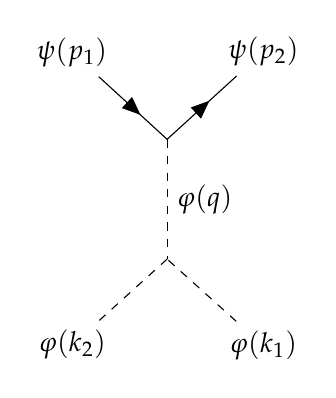
\begin{tikzpicture}
    \begin{feynman}
        \diagram [vertical=a to b] {
            i1 [particle=\(\psi(p_1)\)] -- [fermion] a -- [fermion] i2 [particle=\(\psi(p_2)\)],
            a -- [scalar, edge label=\(\varphi(q)\)] b,
            f1 [particle=\(\varphi(k_1)\)] -- [scalar] b -- [scalar] f2 [particle=\(\varphi(k_2)\)],
        };
    \end{feynman}
\end{tikzpicture}
\end{center}
From the interaction term $L_{\text{int}} = -g \psi^* \psi \varphi$, the vertex factor is $-ig$. The propagator for the exchanged $\varphi$ field is given by:
\begin{align}
    \frac{i}{q^2 - m^2 + i\epsilon}, \label{eq:var-phi-propagator}
\end{align}
where $q = p_1 - p_2$ is the momentum transfer.

The total scattering amplitude $\mathcal{M}$ for this process is given by the product of the vertex factors and the propagator:
\begin{align}
    \mathcal{M} &= (-ig)^2 \cdot \frac{i}{q^2 - m^2 + i\epsilon} \nonumber \\
    &= \frac{-g^2 i}{q^2 - m^2 + i\epsilon}, \label{eq:total-amplitude}
\end{align}
where $q^2 = (p_1 - p_2)^2$ is the Mandelstam variable for the momentum transfer.
\item [(b)] Scattering Amplitude for $\psi \psi^* \rightarrow \varphi \varphi$.

At leading order, the process $\psi \psi^* \rightarrow \varphi \varphi$ occurs via a $\varphi$ exchange in the s-channel:
\[
\psi(p_1) + \psi^*(p_2) \rightarrow \varphi(k_1) + \varphi(k_2)
\]
The Feynman diagram is:
\begin{center}
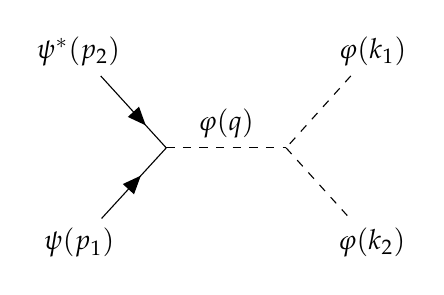
\begin{tikzpicture}
    \begin{feynman}
        \diagram [horizontal=a to b] {
            i1 [particle=\(\psi(p_1)\)] -- [fermion] a -- [anti fermion] i2 [particle=\(\psi^*(p_2)\)],
            a -- [scalar, edge label=\(\varphi(q)\)] b,
            f1 [particle=\(\varphi(k_1)\)] -- [scalar] b -- [scalar] f2 [particle=\(\varphi(k_2)\)],
        };
    \end{feynman}
\end{tikzpicture}
\end{center}
As before, the vertex factor is $-ig$, and the propagator for the exchanged $\varphi$ field is:
\begin{align}
    \frac{i}{q^2 - m^2 + i\epsilon}, 
\end{align}
where $q = p_1 + p_2 = k_1 + k_2$ is the total energy in the center-of-mass frame.

The scattering amplitude $\mathcal{M}$ for this process is:
\begin{align}
    \mathcal{M} &= (-ig)^2 \cdot \frac{i}{q^2 - m^2 + i\epsilon} \nonumber \\
    &= \frac{-g^2 i}{q^2 - m^2 + i\epsilon},
\end{align}
where $q^2 = (p_1 + p_2)^2$ is the Mandelstam variable in the s-channel.
\end{enumerate}
\bigskip\bigskip\hline\hline\bigskip
% \allowdisplaybreaks
\begin{center}
	\hrule
	\vspace{.4cm}
 \begin{tabular*}{\textwidth}{@{}l@{}|@{\extracolsep{0.6in}}r@{}}%
\parbox{4.25in}{\raggedright{
\includegraphics[width=.9\linewidth]{ictp-pwf.pdf}}} &
\parbox[c][]{4in}{{\Large\textbf{Md Akiful Islam Zawad} \par}
                    { Brac University \par}
                    { KHA 224, Progati Sarani, Merul Badda, \par}
                    { Dhaka 1212, Bangladesh \par}
                    { \href{ext.akiful.islam@bracu.ac.bd}{ext.akiful.islam@bracu.ac.bd}} \par}
\end{tabular*}\vspace{.3in}
\definecolor{ceruleanblue}{rgb}{0.16, 0.32, 0.6}
	\LARGE\scshape\textbf{\textcolor{ceruleanblue}{Physics for Bangladesh QFT School}}
\end{center}
\hrule\vspace{.25in}
{\large\textbf{Problem Sheet:}\ \textsc{4} \hspace{\hfill} \large\textbf{Due Date:} \today\\
	\hrule}
 %----------------------------
\paragraph*{Problem Set 2} %\hfill \newline
\\
Use the properties 
\begin{align}
    \{ \gamma^\mu, \gamma^\nu \} = 2\eta^{\mu\nu} \quad \text{and} \quad \text{(ii) cyclic property of trace},\label{eq:given-properties}
\end{align}
to do the following:

\begin{itemize}
    \item[(a)] Show that the trace of any odd number of $\gamma^\mu$ ($\mu = 0, 1, 2, 3$) is zero.
    \item[(b)] Find an expression for $\text{Tr}(\gamma^\mu \gamma^\nu \gamma^\rho \gamma^\sigma)$ in terms of the Minkowski metric.
    \item[(c)] Find an expression for $\text{Tr}(\gamma^\mu \gamma^\nu \gamma^\rho \gamma^\sigma \gamma^\alpha \gamma^\beta)$.
    \item[(d)] Can you guess how many additive terms it will have in the expression for the trace of eight $\gamma^\mu$ matrices?
\end{itemize}
\bigskip\bigskip\hline\hline\bigskip
\begin{enumerate}
    \item [(a)] We are only given to use (\ref{eq:given-properties}) to solve this question. The cyclic property of the trace, is 
    \begin{align}
        tr\left(A\ldots BC\right)=tr\left(CA\ldots B\right)
    \end{align}
    We also get to use $\displaystyle\gamma_5^2=1$ and $\left\{\gamma_5,\gamma^\alpha\right\}=0$
    \begin{align}
        tr\left(\underbrace{\gamma^\alpha\ldots\gamma^\beta}_{2n+1}\right)&=tr\left(1\gamma^\alpha\ldots\gamma^\beta\right)\notag\\
        &=tr\left(\gamma_5\gamma_5\gamma^\alpha\ldots\gamma^\beta\right)\notag\\
        &=-tr\left(\gamma_5\gamma^\alpha\gamma_5\ldots\gamma^\beta\right)\notag\\
        &=(-1)^{2n+1}tr\left(\gamma_5\gamma^\alpha\ldots\gamma^\beta\gamma_5\right)\notag\\
        &=(-1)^{2n+1}\left(\gamma_5\gamma_5\gamma^\alpha\ldots\gamma^\beta\right)\notag\\
        &=-tr\left(\gamma^\alpha\ldots\gamma^\beta\right)\notag\\
        &=0
    \end{align}
    \item [(b)] We start with the trace product of $2$ gamma matrices.
    \begin{align}
        tr\left(\gamma^\mu\gamma^\nu\right)&=tr\left(-\gamma^\nu\gamma^\mu+2\eta^{\mu\nu}1\right)\notag\\
        &=-tr\left(\gamma^\nu\gamma^\mu\right)+2\eta^{\mu\nu}tr(1)\notat\\
        &=-tr\left(\gamma^\mu\gamma^\nu\right)+8\eta^{\mu\nu}\notag\\
        &=4\eta^{\mu\nu}.
    \end{align}
    We can use this to evaluate the trace products of $4$ gamma matrices.
    \begin{align}
        tr\left(\gamma^\mu\gamma^\nu\gamma^\rho\gamma^\sigma\right)&=tr\left(\left(-\gamma^\nu\gamma^\mu+2\eta^{\mu\nu}1\right)\gamma^\rho\gamma^\sigma\right)\notag\\
        &=-tr\left(\gamma^\nu\gamma^\mu\gamma^\rho\gamma^\sigma\right)+2\eta^{\mu\nu}tr\left(\gamma^\rho\gamma^\sigma\right)\notag\\
        &=-tr\left(\gamma^\nu\left(-\gamma^\rho\gamma^\mu+2\eta^{\mu\rho}\gamma^\sigma\right)\right)+2\eta^{\mu\nu}tr\left(\gamma^\rho\gamma^\sigma\right)\notag\\
        &=tr\left(\gamma^\nu\gamma^\rho\gamma^\mu\gamma^\sigma\right)-2\eta^{\mu\rho}tr\left(\gamma^\nu\gamma^\sigma\right)+2\eta^{\mu\nu}tr\left(\gamma^\rho\gamma^\sigma\right)\notag\\
        &=tr\left(\gamma^\nu\gamma^\rho\left(-\gamma^\sigma\gamma^\mu\right)+2\eta^{\sigma\mu}\right)-2\eta^{\mu\rho}tr\left(\gamma^\nu\gamma^\sigma\right)+2\eta^{\mu\nu}tr\left(\gamma^\rho\gamma^\sigma\right)\notag\\
        &=-tr\left(\gamma^\nu\gamma^\rho\gamma^\sigma\gamma^\mu\right)+2\eta^{\sigma\mu}tr\left(\gamma^\nu\gamma^\rho\right)-2\eta^{\mu\rho}tr\left(\gamma^\nu\gamma^\sigma\right)+2\eta^{\mu\nu}tr\left(\gamma^\rho\gamma^\sigma\right)\notag\\
        2tr\left(\gamma^\mu\gamma^\nu\gamma^\rho\gamma^\sigma\right)&=2\eta^{\sigma\mu}tr\left(\gamma^\nu\gamma^\rho\right)-2\eta^{\mu\rho}tr\left(\gamma^\nu\gamma^\sigma\right)+2\eta^{\mu\nu}tr\left(\gamma^\rho\gamma^\sigma\right)\notag\\
        \therefore tr\left(\gamma^\mu\gamma^\nu\gamma^\rho\gamma^\sigma\right)&=4\eta^{\sigma\mu}\eta^{\nu\rho}-4\eta^{\mu\rho}\eta^{\nu\sigma}+4\eta^{\mu\nu}\eta^{\rho\sigma}\label{eq:4-gamma-matrices-mu-nu}
    \end{align}
    \item [(c)] For a trace product of six gamma matrices, we use (\ref{eq:4-gamma-matrices-mu-nu}) to speed up the process:
    \begin{align}
        tr\left(\gamma^\mu\gamma^\nu\gamma^\rho\gamma^\sigma\gamma^\alpha\gamma^\beta\right)&=tr\left(\left(-\gamma^\nu\gamma^\mu+2\eta^{\mu\nu}1\right)\gamma^\rho\gamma^\sigma\gamma^\alpha\gamma^\beta\right)\notag\\
        &=tr\left(-\gamma^\nu\left(2\eta^{\mu\rho}-\gamma^\rho\gamma^\mu\right)\gamma^\sigma\gamma^\alpha\gamma^\beta+2\eta^{\mu\nu}\gamma^\rho\gamma^\sigma\gamma^\alpha\gamma^\beta\right)\notag\\
        &=tr\left(-\gamma^\nu\gamma^\rho\gamma^\sigma\gamma^\alpha\gamma^\beta\gamma^\mu+2\eta^{\mu\rho}\gamma^\nu\gamma^\sigma\gamma^\alpha\gamma^\beta-2\eta^{\mu\sigma}\gamma^\nu\gamma^\rho\gamma^\alpha\gamma^\beta\right.\notag\\
        &\left.\hspace{50pt}+2\eta^{\mu\alpha}\gamma^\nu\gamma^\rho\gamma^\sigma\gamma^\beta-2\eta^{\mu\beta}\gamma^\nu\gamma^\rho\gamma^\sigma\gamma^\alpha+2\eta^{\mu\nu}\gamma^\rho\gamma^\sigma\gamma^\alpha\gamma^\beta\right)\notat\\
        &=tr\left(\eta^{\mu\sigma}\gamma^\nu\gamma^\rho\gamma^\alpha\gamma^\beta-\eta^{\mu\alpha}\gamma^\nu\gamma^\rho\gamma^\sigma\gamma^\beta+\eta^{\mu\rho}\gamma^\nu\gamma^\sigma\gamma^\alpha\gamma^\beta-\eta^{\mu\beta}\gamma^\nu\gamma^\rho\gamma^\sigma\gamma^\alpha+\eta^{\mu\nu}\gamma^\rho\gamma^\sigma\gamma^\alpha\gamma^\beta\right)\notag\\
        &=4\eta^{\mu\alpha}\left(\eta^{\nu\rho}\eta^{\sigma\beta}-\eta^{\nu\sigma}\eta^{\rho\beta}+\eta^{\beta\nu}\eta^{\rho\sigma}\right)-4\eta^{\mu\sigma}\left(\eta^{\nu\rho}\eta^{\alpha\beta}-\eta^{\nu\alpha}\eta^{\rho\beta}+\eta^{\beta\nu}\eta^{\rho\alpha}\right)\notag\\
        &\hspace{40pt}4\eta^{\mu\rho}\left(\eta^{\nu\sigma}\eta^{\alpha\beta}-\eta^{\nu\alpha}\eta^{\sigma\beta}+\eta^{\beta\sigma}\eta^{\nu\alpha}\right)-4\eta^{\mu\alpha}\left(\eta^{\nu\rho}\eta^{\sigma\beta}-\eta^{\nu\beta}\eta^{\rho\sigma}\right)\notag\\
        &\hspace{60pt}4\eta^{\mu\nu}\left(\eta^{\rho\sigma}\eta^{\alpha\beta}-\eta^{\rho\alpha}\eta^{\beta\sigma}+\eta^{\rho\beta}\eta^{\alpha\sigma}\right)\label{eq:six-matrices}
    \end{align}
    \item [(d)] Now move on to the trace of the product of 8 gamma matrices $\gamma^\mu \gamma^\nu \gamma^\rho \gamma^\sigma \gamma^\alpha \gamma^\beta \gamma^\delta \gamma^\epsilon$. Using the strategy from previous calculations, we use the anticommutation relations to reduce the number of gamma matrices.
    \begin{align}
        tr\left(\gamma^\mu \gamma^\nu \gamma^\rho \gamma^\sigma \gamma^\alpha \gamma^\beta \gamma^\delta \gamma^\epsilon\right) &= tr\left(\left(-\gamma^\nu \gamma^\mu + 2 \eta^{\mu\nu}1\right) \gamma^\rho \gamma^\sigma \gamma^\alpha \gamma^\beta \gamma^\delta \gamma^\epsilon\right)\notag\\
        &= tr\left(-\gamma^\nu \left( -\gamma^\rho \gamma^\mu + 2 \eta^{\mu\rho} \right) \gamma^\sigma \gamma^\alpha \gamma^\beta \gamma^\delta \gamma^\epsilon + 2 \eta^{\mu\nu} \gamma^\rho \gamma^\sigma \gamma^\alpha \gamma^\beta \gamma^\delta \gamma^\epsilon \right)\notag\\
        &= tr\left( -\gamma^\nu \gamma^\rho \gamma^\sigma \gamma^\alpha \gamma^\beta \gamma^\delta \gamma^\epsilon \gamma^\mu + 2 \eta^{\mu\rho} \gamma^\nu \gamma^\sigma \gamma^\alpha \gamma^\beta \gamma^\delta \gamma^\epsilon + 2 \eta^{\mu\nu} \gamma^\rho \gamma^\sigma \gamma^\alpha \gamma^\beta \gamma^\delta \gamma^\epsilon \right)\notag\\
        &= tr\left( -\gamma^\nu \gamma^\rho \gamma^\sigma \gamma^\alpha \gamma^\beta \gamma^\delta \gamma^\epsilon \gamma^\mu \right) + 2 \eta^{\mu\rho} tr\left( \gamma^\nu \gamma^\sigma \gamma^\alpha \gamma^\beta \gamma^\delta \gamma^\epsilon \right) + 2 \eta^{\mu\nu} tr\left( \gamma^\rho \gamma^\sigma \gamma^\alpha \gamma^\beta \gamma^\delta \gamma^\epsilon \right)\notag
    \end{align}
    From here on ahead, we apply the same procedure iteratively to further reduce the number of gamma matrices. When working with gamma matrices, we use the anticommutation relation to replace the product of two gamma matrices by the Minkowski metric (\ref{eq:given-properties}). Each time we apply this relation, we reduce the number of gamma matrices by 2 and introduce a term proportional to the Minkowski metric $\eta^{\mu\nu}$.  
    
    For 8 gamma matrices, we can apply the anticommutation relation iteratively until all gamma matrices are paired off. Any unpaired gamma matrices will vanish because the trace of an odd number of gamma matrices is zero.
    \begin{align}
        tr\left(\gamma^\mu \gamma^\nu \gamma^\rho \gamma^\sigma \gamma^\alpha \gamma^\beta \gamma^\delta \gamma^\epsilon\right) &= 4 \left( \eta^{\mu\nu} \eta^{\rho\sigma} \eta^{\alpha\beta} \eta^{\delta\epsilon} - \eta^{\mu\rho} \eta^{\nu\sigma} \eta^{\alpha\beta} \eta^{\delta\epsilon} + \eta^{\mu\sigma} \eta^{\nu\rho} \eta^{\alpha\beta} \eta^{\delta\epsilon} + \dots \right) \notag
    \end{align}
    The next step is to count how many ways we can contract the 8 indices into pairs. We start with the indices $\mu, \nu, \rho, \sigma, \alpha, \beta, \delta, \epsilon$. Each pair of indices corresponds to a factor of the Minkowski metric $\eta^{\mu\nu}$. We can pair the first index, $\mu$, with any of the remaining 7 indices: $\nu, \rho, \sigma, \alpha, \beta, \delta, \epsilon$. This gives us 7 possible choices for the first pair. After making the first pair, we are left with 6 indices. The second index can be paired with any of the remaining 5 indices, giving us 5 choices for the second pair.
    
    We continue this process until all indices are paired off. After making 4 pairs, all the indices will be contracted.
    
    The total number of ways to pair off 8 indices is given by the combinatorial formula:
    \begin{align}
        \text{Number of pairings} &= \frac{8!}{4! 2^4}\notag\\
        &= \frac{40320}{24 \times 16} \notag\\
        &= \frac{40320}{384} \notag\\
        &= 105.
    \end{align}
    This formula accounts for the following factors:
    \begin{itemize}
        \item The term $8!$ counts all possible ways to permute the 8 indices.
        \item The term $4!$ corrects for the fact that the order of the 4 pairs does not matter.
        \item The term $2^4$ corrects for the fact that within each pair, the order of the two indices does not matter (i.e., $\eta^{\mu\nu} = \eta^{\nu\mu}$).
    \end{itemize}
    Thus, there are 105 distinct ways to fully contract the 8 indices using the Minkowski metric.
\end{enumerate}
\bigskip\bigskip\hline\hline\bigskip
% \allowdisplaybreaks
\begin{center}
	\hrule
	\vspace{.4cm}
 \begin{tabular*}{\textwidth}{@{}l@{}|@{\extracolsep{0.6in}}r@{}}%
\parbox{4.25in}{\raggedright{
\includegraphics[width=.9\linewidth]{ictp-pwf.pdf}}} &
\parbox[c][]{4in}{{\Large\textbf{Md Akiful Islam Zawad} \par}
                    { Brac University \par}
                    { KHA 224, Progati Sarani, Merul Badda, \par}
                    { Dhaka 1212, Bangladesh \par}
                    { \href{ext.akiful.islam@bracu.ac.bd}{ext.akiful.islam@bracu.ac.bd}} \par}
\end{tabular*}\vspace{.3in}
\definecolor{ceruleanblue}{rgb}{0.16, 0.32, 0.6}
	\LARGE\scshape\textbf{\textcolor{ceruleanblue}{Physics for Bangladesh QFT School}}
\end{center}
\hrule\vspace{.25in}
{\large\textbf{Problem Sheet:}\ \textsc{4} \hspace{\hfill} \large\textbf{Due Date:} \today\\
	\hrule}
 %----------------------------
\paragraph*{Problem Set 3} %\hfill \newline
\\
The Lagrangian for QED is given by
\begin{align}
    L = -\frac{1}{4} F_{\mu\nu} F^{\mu\nu} + \bar{\psi}(i\not{\partial} - m)\psi - e \bar{\psi} \gamma^\mu A_\mu \psi. 
\end{align}
Using the Feynman rules stated in the lecture, please find the leading order scattering amplitude for the following:
\begin{itemize}
    \item[(a)] Compton Scattering: $e^- \gamma \rightarrow e^- \gamma$
    \item[(b)] Bhabha Scattering: $e^- e^+ \rightarrow e^- e^+$
\end{itemize}
\bigskip\bigskip\hline\hline\bigskip
The Feynman rules for the photon, electron, and the interaction between them from this Lagrangian.

The photon part of the Lagrangian is:
\begin{align*}
    L_{\text{photon}} = -\frac{1}{4} F_{\mu\nu} F^{\mu\nu}.
\end{align*}
We express $F_{\mu\nu}$ in terms of the photon field $A_\mu$:
\begin{align*}
    F_{\mu\nu} = \partial_\mu A_\nu - \partial_\nu A_\mu.
\end{align*}
Substituting this into the Lagrangian, we get:
\begin{align*}
    L_{\text{photon}} = -\frac{1}{4} \left( \partial_\mu A_\nu - \partial_\nu A_\mu \right) \left( \partial^\mu A^\nu - \partial^\nu A^\mu \right). 
\end{align*}
This is a quadratic term in $A_\mu$, so we can extract the photon propagator from this part of the Lagrangian. The propagator for the photon is given by:
\begin{align}
    \frac{-i g_{\mu\nu}}{q^2 + i \epsilon},\label{eq:photon-propagator}
\end{align}
where $q$ is the photon 4-momentum and $g_{\mu\nu}$ is the Minkowski metric.

The electron part of the Lagrangian is:
\begin{align*}
    L_{\text{electron}} = \bar{\psi} (i \slashed{\partial} - m) \psi. 
\end{align*}
This is a quadratic term in the spinor field $\psi$. The electron propagator is obtained from the equation of motion derived from this term. The propagator for the electron (or positron) is:
\begin{align}
    \frac{i (\slashed{p} + m)}{p^2 - m^2 + i \epsilon}, \label{eq:electron-propagator}
\end{align}
where $p$ is the electron 4-momentum and $m$ is the electron mass.

The interaction term in the Lagrangian is:
\begin{align}
    L_{\text{int}} = - e \bar{\psi} \gamma^\mu A_\mu \psi. \label{eq:interaction-lagrangian}
\end{align}
This describes the interaction between the electron and the photon. From this term, we can directly extract the Feynman rule for the vertex involving one incoming electron, one outgoing electron, and one photon.

The Feynman rule for the vertex corresponding to this interaction is:
\begin{align}
    \text{Vertex factor: } -i e \gamma^\mu,\label{eq:vertex-factor}
\end{align}
\begin{enumerate}
    \item [(a)] Compton Scattering: $e^- \gamma \rightarrow e^- \gamma$
At leading order, the process $e^- \gamma \rightarrow e^- \gamma$ occurs via two Feynman diagrams:
\begin{itemize}
    \item s-channel: An electron is annihilated by the incoming photon and then propagates before emitting a photon and becoming the outgoing electron.
    \item t-channel: The incoming electron absorbs the photon, becomes an intermediate electron, and then emits the photon to become the outgoing electron.
\end{itemize}
The diagrams are:
\begin{figure}[h!]
    \centering
    \begin{subfigure}[b]{0.45\textwidth}
        \centering
        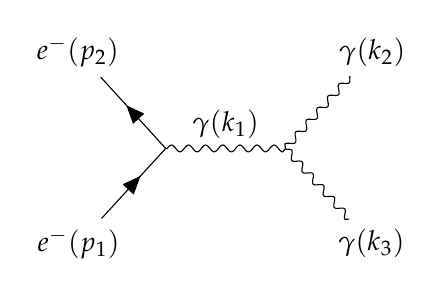
\begin{tikzpicture}
            \begin{feynman}
                \diagram [horizontal=a to b] {
                    i1 [particle=\(e^-(p_1)\)] -- [fermion] a -- [fermion] f1 [particle=\(e^-(p_2)\)],
                    a -- [photon, edge label=\(\gamma(k_1)\)] b,
                    i2 [particle=\(\gamma(k_2)\)] -- [photon] b -- [photon] f2 [particle=\(\gamma(k_3)\)],
                };
            \end{feynman}
        \end{tikzpicture}
        \caption{s-channel for Compton scattering}
    \end{subfigure}
    \hfill
    \begin{subfigure}[b]{0.45\textwidth}
        \centering
        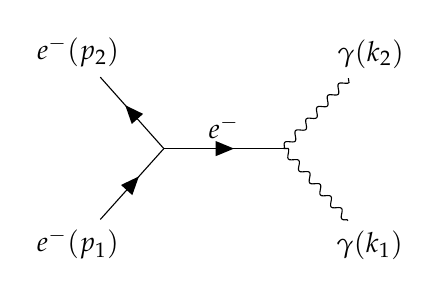
\begin{tikzpicture}
            \begin{feynman}
                \diagram [horizontal=a to b] {
                    i1 [particle=\(e^-(p_1)\)] -- [fermion] a -- [fermion] f1 [particle=\(e^-(p_2)\)],
                    i2 [particle=\(\gamma(k_1)\)] -- [photon] b -- [photon] f2 [particle=\(\gamma(k_2)\)],
                    a -- [fermion, edge label=\(e^-\)] b,
                };
            \end{feynman}
        \end{tikzpicture}
        \caption{t-channel for Compton scattering}
    \end{subfigure}
    \caption{Feynman diagrams for Compton scattering: s-channel and t-channel.}
\end{figure}
From the QED Lagrangian, we recall the Feynman rules (\ref{eq:photon-propagator}), (\ref{eq:electron-propagator}), (\ref{eq:vertex-factor}).

In the s-channel, an electron is annihilated by a photon, propagates as an intermediate electron, and emits a photon. The total amplitude for this diagram is:
\begin{align}
    \mathcal{M}_s &= (-ie) \bar{u}(p_2) \gamma^\mu \frac{i(\slashed{p} + m)}{p^2 - m^2 + i\epsilon} (-ie) \gamma^\nu u(p_1) \varepsilon_\mu(k_1) \varepsilon^*_\nu(k_2), \label{eq:s-channel}
\end{align}
where $p = p_1 + k_1$ is the intermediate electron momentum, and $\varepsilon_\mu(k_1)$ and $\varepsilon^*_\nu(k_2)$ are the polarization vectors of the incoming and outgoing photons, respectively.

Simplifying:
\begin{align}
    \mathcal{M}_s &= \frac{e^2}{p^2 - m^2 + i\epsilon} \bar{u}(p_2) \gamma^\mu (\slashed{p} + m) \gamma^\nu u(p_1) \varepsilon_\mu(k_1) \varepsilon^*_\nu(k_2).
\end{align}
In the t-channel, the electron absorbs a photon, propagates as an intermediate electron, and emits a photon. The amplitude for this diagram is:
\begin{align}
    \mathcal{M}_t &= (-ie) \bar{u}(p_2) \gamma^\nu \frac{i(\slashed{p'} + m)}{p'^2 - m^2 + i\epsilon} (-ie) \gamma^\mu u(p_1) \varepsilon_\mu(k_1) \varepsilon^*_\nu(k_2), \label{eq:t-channel}
\end{align}
where $p' = p_1 - k_2$ is the intermediate electron momentum.

Simplifying:
\begin{align}
    \mathcal{M}_t &= \frac{e^2}{p'^2 - m^2 + i\epsilon} \bar{u}(p_2) \gamma^\nu (\slashed{p'} + m) \gamma^\mu u(p_1) \varepsilon_\mu(k_1) \varepsilon^*_\nu(k_2).
\end{align}
The total amplitude for Compton scattering is the sum of the s-channel (\ref{eq:s-channel}) and t-channel (\ref{eq:t-channel}) amplitudes:
\begin{align*}
    \mathcal{M} = \mathcal{M}_s + \mathcal{M}_t.
\end{align*}
Thus, the leading order scattering amplitude for Compton scattering is given by:
\begin{align}
    \mathcal{M} &= \frac{e^2}{(p_1 + k_1)^2 - m^2 + i\epsilon} \bar{u}(p_2) \gamma^\mu (\slashed{p_1 + k_1} + m) \gamma^\nu u(p_1) \varepsilon_\mu(k_1) \varepsilon^*_\nu(k_2) \nonumber \\
    &\quad + \frac{e^2}{(p_1 - k_2)^2 - m^2 + i\epsilon} \bar{u}(p_2) \gamma^\nu (\slashed{p_1 - k_2} + m) \gamma^\mu u(p_1) \varepsilon_\mu(k_1) \varepsilon^*_\nu(k_2).
\end{align}
\item [(b)] Bhabha Scattering: $e^- e^+ \rightarrow e^- e^+$
At leading order, the process $e^- e^+ \rightarrow e^- e^+$ occurs via two Feynman diagrams:
\begin{itemize}
    \item s-channel: The electron and positron annihilate into a photon, which decays into an electron-positron pair.
    \item t-channel: The electron exchanges a photon with the positron.
\end{itemize}
The diagrams are:
\begin{figure}[h!]
    \centering
    \begin{subfigure}[b]{0.45\textwidth}
        \centering
        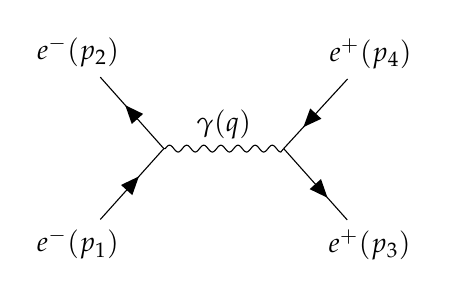
\begin{tikzpicture}
            \begin{feynman}
                \diagram [horizontal=a to b] {
                    i1 [particle=\(e^-(p_1)\)] -- [fermion] a -- [fermion] f1 [particle=\(e^-(p_2)\)],
                    i2 [particle=\(e^+(p_3)\)] -- [anti fermion] b -- [anti fermion] f2 [particle=\(e^+(p_4)\)],
                    a -- [photon, edge label=\(\gamma(q)\)] b,
                };
            \end{feynman}
        \end{tikzpicture}
        \caption{s-channel for Bhabha scattering}
    \end{subfigure}
    \hfill
    \begin{subfigure}[b]{0.45\textwidth}
        \centering
        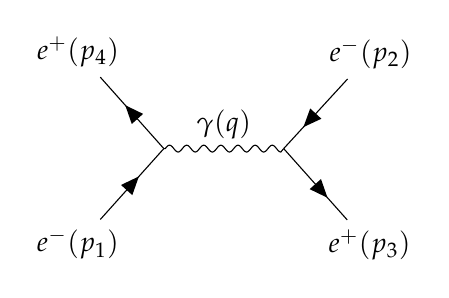
\begin{tikzpicture}
            \begin{feynman}
                \diagram [horizontal=a to b] {
                    i1 [particle=\(e^-(p_1)\)] -- [fermion] a -- [fermion] f2 [particle=\(e^+(p_4)\)],
                    i2 [particle=\(e^+(p_3)\)] -- [anti fermion] b -- [anti fermion] f1 [particle=\(e^-(p_2)\)],
                    a -- [photon, edge label=\(\gamma(q)\)] b,
                };
            \end{feynman}
        \end{tikzpicture}
        \caption{t-channel for Bhabha scattering}
    \end{subfigure}
    \caption{Feynman diagrams for Bhabha scattering: s-channel and t-channel.}
\end{figure}
In the s-channel, the electron and positron annihilate into a photon, which decays into an electron-positron pair. The amplitude for this diagram is:
\begin{align}
    \mathcal{M}_s &= (-ie) \bar{v}(p_2) \gamma^\mu u(p_1) \frac{-ig_{\mu\nu}}{q^2 + i\epsilon} (-ie) \bar{u}(p_3) \gamma^\nu v(p_4), \label{eq:s-channel-bhabha}
\end{align}
where $q = p_1 + p_2$ is the photon momentum in the s-channel.

Simplifying:
\begin{align}
    \mathcal{M}_s &= \frac{e^2}{q^2 + i\epsilon} \bar{v}(p_2) \gamma^\mu u(p_1) \bar{u}(p_3) \gamma_\mu v(p_4).
\end{align}
In the t-channel, the electron and positron exchange a photon. The amplitude for this diagram is:
\begin{align}
    \mathcal{M}_t &= (-ie)^2 \bar{u}(p_3) \gamma^\mu \frac{i(\slashed{p} + m)}{p^2 - m^2 + i\epsilon} \gamma^\nu u(p_1) \bar{v}(p_2) \gamma_\mu v(p_4), \label{eq:t-channel-bhabha}
\end{align}
where $p = p_1 - p_3$ is the momentum exchanged in the t-channel.

Simplifying:
\begin{align}
    \mathcal{M}_t &= \frac{e^2}{p^2 - m^2 + i\epsilon} \bar{u}(p_3) \gamma^\mu (\slashed{p} + m) \gamma^\nu u(p_1) \bar{v}(p_2) \gamma_\mu v(p_4).
\end{align}
The total amplitude for Bhabha scattering is the sum of the s-channel (\ref{eq:s-channel-bhabha}) and t-channel (\ref{eq:t-channel-bhabha}) amplitudes:
\begin{align*}
    \mathcal{M} = \mathcal{M}_s + \mathcal{M}_t.
\end{align*}
Thus, the leading order scattering amplitude for Bhabha scattering is given by:
\begin{align}
    \mathcal{M} &= \frac{e^2}{(p_1 + p_2)^2 + i\epsilon} \bar{v}(p_2) \gamma^\mu u(p_1) \bar{u}(p_3) \gamma_\mu v(p_4) \nonumber \\
    &\quad + \frac{e^2}{(p_1 - p_3)^2 - m^2 + i\epsilon} \bar{u}(p_3) \gamma^\mu (\slashed{p_1 - p_3} + m) \gamma^\nu u(p_1) \bar{v}(p_2) \gamma_\mu v(p_4).
\end{align}
\end{enumerate}
\bigskip\bigskip\hline\hline\bigskip
% \allowdisplaybreaks
\begin{center}
	\hrule
	\vspace{.4cm}
 \begin{tabular*}{\textwidth}{@{}l@{}|@{\extracolsep{0.6in}}r@{}}%
\parbox{4.25in}{\raggedright{
\includegraphics[width=.9\linewidth]{ictp-pwf.pdf}}} &
\parbox[c][]{4in}{{\Large\textbf{Md Akiful Islam Zawad} \par}
                    { Brac University \par}
                    { KHA 224, Progati Sarani, Merul Badda, \par}
                    { Dhaka 1212, Bangladesh \par}
                    { \href{ext.akiful.islam@bracu.ac.bd}{ext.akiful.islam@bracu.ac.bd}} \par}
\end{tabular*}\vspace{.3in}
\definecolor{ceruleanblue}{rgb}{0.16, 0.32, 0.6}
	\LARGE\scshape\textbf{\textcolor{ceruleanblue}{Physics for Bangladesh QFT School}}
\end{center}
\hrule\vspace{.25in}
{\large\textbf{Problem Sheet:}\ \textsc{4} \hspace{\hfill} \large\textbf{Due Date:} \today\\
	\hrule}
 %----------------------------
\paragraph*{Problem Set 4} %\hfill \newline
\\
The Lagrangian for Scalar QED (complex scalar field $\varphi$ interacting with field $A_\mu$) is given by
\begin{align}
    L = -\frac{1}{4} F_{\mu\nu}^2 + (D_\mu \varphi)^* (D^\mu \varphi) - m^2 \varphi^* \varphi, 
\end{align}
where $D_\mu = \partial_\mu + ieA_\mu$ is the usual gauge-covariant derivative.
\begin{itemize}
    \item[(a)] Compute the Interaction Lagrangian.
    \item[(b)] Derive the Feynman rules for the vertices and propagators of the above theory.
\end{itemize}
\bigskip\bigskip\hline\hline\bigskip
\begin{enumerate}
    \item [(a)] Compute the Interaction Lagrangian

The covariant derivative $D_\mu = \partial_\mu + ie A_\mu$ is used to describe how the scalar field $\varphi$ interacts with the photon field $A_\mu$. The kinetic term in the Lagrangian is written as:
\begin{align}
    (D_\mu \varphi)^* (D^\mu \varphi) &= \left( \partial_\mu \varphi^* - ie A_\mu \varphi^* \right) \left( \partial^\mu \varphi + ie A^\mu \varphi \right).
\end{align}
This expression expands into four terms, representing the kinetic energy of the scalar field, the interaction between the scalar field and the photon, and a photon-photon-scalar interaction.

We now expand the expression for $(D_\mu \varphi)^* (D^\mu \varphi)$ to reveal all the terms:
\begin{align}
    (D_\mu \varphi)^* (D^\mu \varphi) &= \left( \partial_\mu \varphi^* \partial^\mu \varphi \right) 
    + ie \left( \varphi^* A_\mu \partial^\mu \varphi \right)
    - ie \left( \partial_\mu \varphi^* A^\mu \varphi \right)
    + e^2 \left( A_\mu A^\mu \varphi^* \varphi \right).
\end{align}
Each of these terms has a specific physical meaning:
\begin{itemize}
    \item $\partial_\mu \varphi^* \partial^\mu \varphi$: This term describes the usual kinetic energy of the complex scalar field $\varphi$.
    \item $ie \varphi^* A_\mu \partial^\mu \varphi$: This is an interaction term between the scalar field $\varphi$ and the photon field $A_\mu$. It represents the emission or absorption of a photon by the scalar field.
    \item $-ie \partial_\mu \varphi^* A^\mu \varphi$: This is another interaction term, similar to the previous one, but involving the complex conjugate field $\varphi^*$.
    \item $e^2 A_\mu A^\mu \varphi^* \varphi$: This term represents the interaction between two photons and the scalar field. It describes processes in which two photons interact with the scalar field simultaneously.
\end{itemize}

Now that we have expanded the covariant derivative terms, we can substitute them into the original Lagrangian. The full expression for the Lagrangian becomes:
\begin{align}
    L &= -\frac{1}{4} F_{\mu\nu}^2 + \partial_\mu \varphi^* \partial^\mu \varphi - m^2 \varphi^* \varphi \nonumber \\
    &\quad + ie \varphi^* A_\mu \partial^\mu \varphi - ie \partial_\mu \varphi^* A^\mu \varphi + e^2 A_\mu A^\mu \varphi^* \varphi.
\end{align}
Here, the first term describes the dynamics of the photon field $A_\mu$, the second and third terms describe the dynamics of the scalar field $\varphi$, and the remaining terms represent the interactions between the scalar field and the photon field.

The interaction Lagrangian consists of the terms that describe the interactions between the scalar field and the photon field. These terms are:
\begin{align}
    L_{\text{int}} &= ie \varphi^* A_\mu \partial^\mu \varphi - ie \partial_\mu \varphi^* A^\mu \varphi + e^2 A_\mu A^\mu \varphi^* \varphi. 
\end{align}
This interaction Lagrangian contains two main types of interactions:
\begin{itemize}
    \item The first two terms describe the interaction between the scalar field and a single photon.
    \item The last term describes the interaction between the scalar field and two photons.
\end{itemize}
\item [(b)] Derive the Feynman Rules for Vertices and Propagators

The propagator for the scalar field $\varphi$ can be derived from the free part of the Lagrangian:
\begin{align}
    L_{\text{free}}(\varphi) = \partial_\mu \varphi^* \partial^\mu \varphi - m^2 \varphi^* \varphi.
\end{align}
This is the standard Lagrangian for a complex scalar field. The propagator for the scalar field is given by:
\begin{align}
    \frac{i}{p^2 - m^2 + i\epsilon},
\end{align}
where $p$ is the 4-momentum of the scalar particle, and $m$ is its mass.

The photon propagator is derived from the free part of the Lagrangian for the photon field:
\begin{align}
    L_{\text{free}}(A_\mu) = -\frac{1}{4} F_{\mu\nu}^2,
\end{align}
which gives the propagator for the photon field:
\begin{align}
    \frac{-ig_{\mu\nu}}{q^2 + i\epsilon},
\end{align}
where $q$ is the 4-momentum of the photon.

The terms $ie \varphi^* A_\mu \partial^\mu \varphi$ and $-ie \partial_\mu \varphi^* A^\mu \varphi$ describe the interaction between the scalar field and a single photon. The Feynman rule for the vertex involving one incoming photon and one incoming/outgoing scalar particle is given by:
\begin{align}
    \text{Vertex factor: } \quad ie (p_1^\mu + p_2^\mu), 
\end{align}
where $p_1^\mu$ and $p_2^\mu$ are the 4-momenta of the incoming and outgoing scalar fields.

The term $e^2 A_\mu A^\mu \varphi^* \varphi$ describes the interaction between two photons and the scalar field. The Feynman rule for this vertex, involving two incoming photons and two scalar fields, is given by:
\begin{align}
    \text{Vertex factor: } \quad 2ie^2 g_{\mu\nu},
\end{align}
where $g_{\mu\nu}$ is the metric tensor for the photon-photon interaction.
\end{enumerate}

% \allowdisplaybreaks
\begin{center}
	\hrule
	\vspace{.4cm}
 \begin{tabular*}{\textwidth}{@{}l@{}|@{\extracolsep{0.6in}}r@{}}%
\parbox{4.25in}{\raggedright{
\includegraphics[width=.9\linewidth]{ictp-pwf.pdf}}} &
\parbox[c][]{4in}{{\Large\textbf{Md Akiful Islam Zawad} \par}
                    { Brac University \par}
                    { KHA 224, Progati Sarani, Merul Badda, \par}
                    { Dhaka 1212, Bangladesh \par}
                    { \href{ext.akiful.islam@bracu.ac.bd}{ext.akiful.islam@bracu.ac.bd}} \par}
\end{tabular*}\vspace{.3in}
\definecolor{ceruleanblue}{rgb}{0.16, 0.32, 0.6}
	\LARGE\scshape\textbf{\textcolor{ceruleanblue}{Physics for Bangladesh QFT School}}
\end{center}
\hrule\vspace{.25in}
{\large\textbf{Problem Sheet:}\ \textsc{5} \hspace{\hfill} \large\textbf{Due Date:} \today\\
	\hrule}
 %----------------------------
\paragraph*{Problem Set 1} %\hfill \newline
\\
Prove the \textbf{Fundamental Theorem of Quantum Field Theory}: if $A$ is
an $N \times N$ matrix, and $J$ an $N$-component vector, then
\begin{align}
    \bigints \prod_{i=1}^{N} dx_i e^{\displaystyle \left( -\frac{1}{2} x^T A x + J^T x \right)}
    = (2\pi)^{\displaystyle\frac{N}{2}} \sqrt{\det A} e^{\displaystyle \left( \frac{1}{2} J^T A^{-1} J \right)}
\end{align}

\noindent
\textit{Hint}: diagonalize $A$ to reduce the problem into a series of one-dimensional integrals.
\bigskip\bigskip\hline\hline\bigskip
\subsection*{Solution}
The exponent in the integrand is given by:
\begin{align*}
    -\frac{1}{2} x^T A x + J^T x&=-\frac{1}{2} \left( x^T A x - 2 J^T x \right)
\end{align*}
Let us express it in a more convenient form by completing the square. Note that the term $x^T A x$ is quadratic in $x$, and the term $J^T x$ is linear in $x$. The expression can be completed into a perfect square:
\begin{align}
    -\frac{1}{2} \left( x^T A x - 2 J^T x \right) &= -\frac{1}{2} \left( x - A^{-1} J \right)^T A \left( x - A^{-1} J \right) + \frac{1}{2} J^T A^{-1} J.
\end{align}
To simplify the integral, perform a change of variables. Define a new variable:
\begin{align*}
    y = x - A^{-1} J.
\end{align*}
In terms of $y$, the integral over $x$ becomes an integral over $y$, and the Jacobian of the transformation is 1, since this is a simple translation of coordinates.

Substituting this into the original integral, we get:
\begin{align}
    \bigints \prod_{i=1}^{N} dx_i e^{\displaystyle \left( -\frac{1}{2} x^T A x + J^T x \right)}
    = \bigints \prod_{i=1}^{N} dy_i e^{\displaystyle \left( -\frac{1}{2} y^T A y \right)} e^{\displaystyle \left( \frac{1}{2} J^T A^{-1} J \right)}.
\end{align}
To evaluate the integral, it is useful to diagonalize the matrix $A$. Since $A$ is a symmetric positive-definite matrix, we can diagonalize it via an orthogonal transformation. 

Let $A = O \Lambda O^T$, where $O$ is an orthogonal matrix and $\Lambda$ is a diagonal matrix containing the eigenvalues of $A$.

Under this diagonalization, the quadratic form $y^T A y$ becomes:
\begin{align}
    y^T A y = y^T O \Lambda O^T y = z^T \Lambda z,
\end{align}
where $\displaystyle z = O^T y$. The measure $\displaystyle\prod_{i=1}^{N} dy_i$ transforms as $\displaystyle\prod_{i=1}^{N} dz_i$, with no change in the Jacobian since $O$ is an orthogonal matrix.

Now, the integral becomes a product of independent Gaussian integrals:
\begin{align}
    \bigints \prod_{i=1}^{N} dz_i e^{\displaystyle \left( -\frac{1}{2} \sum_{i=1}^{N} \lambda_i z_i^2 \right)},
\end{align}
where $\lambda_i$ are the eigenvalues of $A$. 

Each integral is of the Gaussian integral $\displaystyle\left(\bigints_{\infty}^{-\infty}e^{-ax^2} dx = \sqrt{\frac{\pi}{a}}\right)$ form:
\begin{align}
    \bigints_{-\infty}^{\infty} dz_i e^{\displaystyle \left( -\frac{1}{2} \lambda_i z_i^2 \right)} &= \sqrt{\frac{2\pi}{\lambda_i}} \notag\\
    &= (2\pi)^{\displaystyle\frac{N}{2}} \prod_{i=1}^{N} \frac{1}{\sqrt{\lambda_i}} \notag\\
    &= (2\pi)^{\displaystyle\frac{N}{2}} \frac{1}{\sqrt{\det A}}.
\end{align}
Put everything together:
\begin{align}
    \bigints \prod_{i=1}^{N} dx_i e^{\displaystyle \left( -\frac{1}{2} x^T A x + J^T x \right)}
    = (2\pi)^{\displaystyle\frac{N}{2}} \frac{1}{\sqrt{\det A}} e^{\displaystyle \left( \frac{1}{2} J^T A^{-1} J \right)}.
\end{align}
This completes the proof of the fundamental theorem of quantum field theory.
\bigskip\bigskip\hline\hline\bigskip
% \allowdisplaybreaks
\begin{center}
	\hrule
	\vspace{.4cm}
 \begin{tabular*}{\textwidth}{@{}l@{}|@{\extracolsep{0.6in}}r@{}}%
\parbox{4.25in}{\raggedright{
\includegraphics[width=.9\linewidth]{ictp-pwf.pdf}}} &
\parbox[c][]{4in}{{\Large\textbf{Md Akiful Islam Zawad} \par}
                    { Brac University \par}
                    { KHA 224, Progati Sarani, Merul Badda, \par}
                    { Dhaka 1212, Bangladesh \par}
                    { \href{ext.akiful.islam@bracu.ac.bd}{ext.akiful.islam@bracu.ac.bd}} \par}
\end{tabular*}\vspace{.3in}
\definecolor{ceruleanblue}{rgb}{0.16, 0.32, 0.6}
	\LARGE\scshape\textbf{\textcolor{ceruleanblue}{Physics for Bangladesh QFT School}}
\end{center}
\hrule\vspace{.25in}
{\large\textbf{Problem Sheet:}\ \textsc{5} \hspace{\hfill} \large\textbf{Due Date:} \today\\
	\hrule}
 %----------------------------
\paragraph*{Problem Set 2} %\hfill \newline
\\
Here we will study the simple harmonic oscillator at finite temperature by evaluating some functional determinants. We will study the quantum harmonic oscillator with Hamiltonian and Lagrangian:
\begin{align}
    H = \frac{p^2}{2} + \frac{1}{2} \omega^2 q^2, \quad L = \frac{1}{2} \dot{q}^2 - \frac{\omega^2}{2} q^2.
\end{align}
\begin{enumerate}
    \item [(a)] The fundamental object in quantum statistical mechanics is the partition function, defined as
\begin{align}
    Z(\beta) = \text{Tr} \, \exp(-\beta H), \label{eq:partition-function-qm-def}
\end{align}
where $H$ is the Hamiltonian of the quantum mechanical system. Use properties of the path integral to convince yourself that the partition function can be computed by the following path integral over compact Euclidean time $\tau$:
\begin{align}
    Z(\beta) = \bigints_{q(0)=q(\beta)} [Dq] \exp \left[ -\bigints_{\,0}^{\beta} d\tau \left( \frac{1}{2} \left( \frac{dq}{d\tau} \right)^2 + \frac{\omega^2}{2} q^2 \right) \right]
\end{align}
where compact Euclidean time means that $\tau \in [0, \beta]$, and the field $q(\tau)$ satisfies periodic boundary conditions, i.e. $q(0) = q(\beta)$. Thus we are doing the functional integral over fields defined on a circle of length $\beta$.
\item [(b)] This functional integral can be evaluated using the “fundamental theorem” above to be the functional determinant
\begin{align}
    Z(\beta) \propto \left[ \det \left( -\frac{d^2}{d\tau^2} + \omega^2 \right) \right]^{-1/2},
\end{align}
where I have omitted $\omega$-independent factors of $(2\pi)^\infty$. Evaluate this determinant and compute the $\omega$-dependence of the partition function. (Getting the $\beta$-dependence exactly right is tricky, but the $\omega$-dependence is unambiguous). You may find the identity
\begin{align}
    \sinh z = z \prod_{n=1}^{\infty} \left( 1 + \frac{z^2}{(n\pi)^2} \right)
\end{align}
useful.

Compare your result to the usual partition function computed via canonical methods (i.e. by directly calculating the sum over the eigenstates of the simple harmonic oscillator in (\ref{eq:partition-function-qm-def}).
\end{enumerate}
\bigskip\bigskip\hline\hline\bigskip
\subsection*{Solution}
\begin{enumerate}
    \item [(a)] The partition function $Z(\beta)$ in quantum statistical mechanics is defined as:
    \begin{align}
        Z(\beta) = \text{Tr} \, \exp(-\beta H),
    \end{align}
    where $H$ is the Hamiltonian of the quantum mechanical system and $\displaystyle\beta = \frac{1}{k_B T}$ represents the inverse temperature. The trace sums over all possible quantum states of the system. However, there is a deep connection between the Boltzmann factor $\exp(-\beta H)$ and time evolution in imaginary time.
    
    To see this, recall that in standard quantum mechanics, the time evolution of a state $| \psi(t) \rangle$ is governed by the Schrödinger equation:
    \begin{align*}
        | \psi(t) \rangle = \exp(-i H t) | \psi(0) \rangle.
    \end{align*}
    By replacing $t$ with imaginary time $\tau = i t$, the time evolution operator becomes $\exp(-H \tau)$. 
    
    In statistical mechanics, this imaginary time evolution occurs over an interval of length $\beta$, as $\beta$ plays the role of inverse temperature. Thus, the partition function is analogous to time evolution in imaginary (Euclidean) time over an interval $[0, \beta]$:
    \begin{align}
        Z(\beta) = \text{Tr} \, \exp(-\beta H) = \bigints_{\displaystyle q(0) = q(\beta)} [Dq] \exp \left[ - \bigints_{~~0}^{\beta} d\tau \, L_E \right],
    \end{align}
    where $L_E$ is the Euclidean Lagrangian.

    Since the trace $\text{Tr}$ sums over all possible quantum states, it implies that the quantum system returns to its original state after time $\tau = \beta$. This is why the fields $q(\tau)$ must satisfy periodic boundary conditions:
    \begin{align}
        q(0) = q(\beta).
    \end{align}
    In other words, the field $q(\tau)$ evolves in imaginary time from $\tau = 0$ to $\tau = \beta$, and because of the trace operation, it “loops back” on itself at $\tau = \beta$, forming a closed path.
    
    The periodic boundary conditions imply that the quantum system evolves in Euclidean time as though it were propagating over a circle of length $\beta$. The interval $\tau \in [0, \beta]$ represents the circumference of the circle. The path integral, therefore, sums over all possible configurations of the field $q(\tau)$ that live on this circle. The circular nature of the path integral arises because the system returns to the same configuration after time $\tau = \beta$, forming a closed loop in imaginary time.
    \begin{itemize}
        \item Imagine a point moving on a straight line in real time. The point moves from some position at $t = 0$ to another position at $t = T$, where $T$ is a finite time.
        \item Now, in imaginary time, instead of a straight line, the point moves on a \textit{loop} from $\tau = 0$ to $\tau = \beta$ and then returns to its original position because of the periodic boundary conditions.
        \item The periodicity in $\tau$ effectively makes the system “wrap around,” creating a circle in imaginary time.
    \end{itemize}
    Thus, the propagation of the quantum system in imaginary time is akin to the system evolving on a circle, where the field configuration at $\tau = 0$ must match the configuration at $\tau = \beta$.
    
    With this understanding, the partition function is given by:
    \begin{align}
        Z(\beta) = \bigints_{\displaystyle q(0) = q(\beta)} [Dq] \exp \left[ -\bigints_{~~0}^{\beta} d\tau \left( \frac{1}{2} \left( \frac{dq}{d\tau} \right)^2 + \frac{\omega^2}{2} q^2 \right) \right].\label{eq:partition-function-def}
    \end{align}
    This path integral describes the propagation of the quantum harmonic oscillator over a \textit{circle} of length $\beta$, with periodic boundary conditions. We now proceed to evaluate this functional integral.
    \item [(b)] The path integral in (\ref{eq:partition-function-def}) can be reduced to a functional determinant using the fundamental theorem of quantum field theory, which relates the Gaussian functional integrals to determinants of differential operators. In this case, the operator in the exponent is:
    \[
    -\frac{d^2}{d\tau^2} + \omega^2.
    \]
    Therefore, the partition function can be written as:
    \begin{align}
        Z(\beta) \propto \left[ \det \left( -\frac{d^2}{d\tau^2} + \omega^2 \right) \right]^{-1/2}.\label{eq:partition-function}
    \end{align}
    Next, we evaluate the determinant of the operator $\displaystyle-\frac{d^2}{d\tau^2} + \omega^2$. The eigenvalues of the differential operator $\displaystyle-\frac{d^2}{d\tau^2}$ with periodic boundary conditions $q(0) = q(\beta)$ are given by:
    \[
    \lambda_n = \left( \frac{2\pi n}{\beta} \right)^2 \quad \text{for} \quad n = 0, \pm 1, \pm 2, \dots
    \]
    Thus, the eigenvalues of $\displaystyle-\frac{d^2}{d\tau^2} + \omega^2$ are:
    \[
    \lambda_n = \left( \frac{2\pi n}{\beta} \right)^2 + \omega^2.
    \]
    The functional determinant can be written as the product over all eigenvalues:
    \begin{align*}
        \det \left( -\frac{d^2}{d\tau^2} + \omega^2 \right) = \prod_{n=-\infty}^{\infty} \bigg[\left( \frac{2\pi n}{\beta} \right)^2 + \omega^2\bigg].
    \end{align*}
    To compute the product, we use the following identity:
    \begin{align*}
        \sinh z = z \prod_{n=1}^{\infty} \left( 1 + \frac{z^2}{n^2 \pi^2} \right).
    \end{align*}
    This allows us to express the product over the eigenvalues as:
    \begin{align*}
        \prod_{n=-\infty}^{\infty} \bigg[\left( \frac{2\pi n}{\beta} \right)^2 + \omega^2 \bigg] = \frac{\displaystyle\sinh\left(\frac{\beta\omega}{2}\right)}{\displaystyle\frac{\beta\omega}{2}}.
    \end{align*}
    Therefore, the determinant becomes:
    \begin{align*}
        \det \left( -\frac{d^2}{d\tau^2} + \omega^2 \right) = \frac{\displaystyle\sinh\left(\frac{\beta\omega}{2}\right)}{\displaystyle\frac{\beta\omega}{2}}.
    \end{align*}
    Substituting the determinant into (\ref{eq:partition-function}), we find that the partition function $Z(\beta)$ is proportional to:
    \begin{align*}
        Z(\beta) \propto \left( \frac{\displaystyle\frac{\beta\omega}{2}}{\displaystyle\sinh\left(\frac{\beta\omega}{2}\right)} \right)^{1/2}.
    \end{align*}
    Thus, the $\omega$-dependence of the partition function is:
    \begin{align}
        Z(\beta) \propto \frac{1}{\displaystyle\sinh\left(\frac{\beta\omega}{2}\right)}.
    \end{align}
    This is the final form of the partition function for the quantum harmonic oscillator at finite temperature, where the $\beta$-dependence describes the inverse temperature, and the $\omega$-dependence is given explicitly.

    Now, let us compute the partition function using the canonical approach, where we directly sum over the eigenstates of the simple harmonic oscillator.

    The energy eigenvalues of the quantum harmonic oscillator are given by:
    \begin{align}
        E_n = \left( n + \frac{1}{2} \right) \omega, \quad n = 0, 1, 2, \dots
    \end{align}
    The partition function is then the sum over all energy eigenstates:
    \begin{align}
        Z(\beta) = \text{Tr} \, \exp(-\beta H) = \sum_{n=0}^{\infty} \exp\bigg[-\beta \left( n + \frac{1}{2} \right) \omega \bigg]. 
    \end{align}
    We can factor the exponentials as:
    \begin{align}
        Z(\beta) &= \sum_{n=0}^{\infty} \exp\left( -\beta n \omega \right) \exp\left( -\frac{\beta \omega}{2} \right) \notag \\
        &= \exp\left( -\frac{\beta \omega}{2} \right)\left[\sum_{n=0}^{\infty} \exp\left( -\beta n \omega \right)\right]\notag\\
        &= \exp\left(\displaystyle-\frac{\beta \omega}{2} \right)\cdot\frac{1}{1 - \exp(-\beta \omega)} \notag \\
        &= \frac{\displaystyle\exp\left( -\frac{\beta \omega}{2} \right)}{1 - \exp(-\beta \omega)}\notag\\
        &= \frac{\displaystyle\exp\left( -\frac{\beta \omega}{2} \right)}{\displaystyle2\sinh\left( \frac{\beta \omega}{2} \right) \exp\left( -\frac{\beta \omega}{2} \right)} \notag \\
        &= \frac{1}{\displaystyle2\sinh\left( \frac{\displaystyle\beta \omega}{2} \right)}\notag\\
        &\propto \frac{1}{\displaystyle\sinh\left(\frac{\beta\omega}{2}\right)}.
    \end{align}
    This result agrees with the $\omega$-dependence obtained from the path integral method, up to a constant factor, which was omitted in the path integral derivation. Both methods yield the same physical dependence on the inverse temperature $\beta$ and the oscillator frequency $\omega$.
\end{enumerate}
\bigskip\bigskip\hline\hline\bigskip
% \allowdisplaybreaks
\begin{center}
	\hrule
	\vspace{.4cm}
 \begin{tabular*}{\textwidth}{@{}l@{}|@{\extracolsep{0.6in}}r@{}}%
\parbox{4.25in}{\raggedright{
\includegraphics[width=.9\linewidth]{ictp-pwf.pdf}}} &
\parbox[c][]{4in}{{\Large\textbf{Md Akiful Islam Zawad} \par}
                    { Brac University \par}
                    { KHA 224, Progati Sarani, Merul Badda, \par}
                    { Dhaka 1212, Bangladesh \par}
                    { \href{ext.akiful.islam@bracu.ac.bd}{ext.akiful.islam@bracu.ac.bd}} \par}
\end{tabular*}\vspace{.3in}
\definecolor{ceruleanblue}{rgb}{0.16, 0.32, 0.6}
	\LARGE\scshape\textbf{\textcolor{ceruleanblue}{Physics for Bangladesh QFT School}}
\end{center}
\hrule\vspace{.25in}
{\large\textbf{Problem Sheet:}\ \textsc{5} \hspace{\hfill} \large\textbf{Due Date:} \today\\
	\hrule}
 %----------------------------
\paragraph*{Problem Set 3} %\hfill \newline
\\
Consider a real scalar field $\varphi(x)$ with the Lagrangian density:
\begin{align}
    L = \frac{1}{2} (\partial_\mu \varphi)(\partial^\mu \varphi) - \frac{1}{2} m^2 \varphi^2.
\end{align}
The path-integral expression for the generating functional $Z[J]$ in the presence of an external source $J(x)$ is:
\begin{align}
    Z[J] = \bigints D\varphi \, \exp \left( i \bigints d^4x \left[ \frac{1}{2} (\partial_\mu \varphi)(\partial^\mu \varphi) - \frac{1}{2} m^2 \varphi^2 + J \varphi \right] \right).
\end{align}
Compute the Feynman propagator $\langle 0 | T \{ \varphi(x) \varphi(y) \} | 0 \rangle$ by evaluating the path integral in the limit of $J(x) \to 0$. Use the result to derive the expression for the propagator in momentum space:
\begin{align}
    \Delta_F(x - y) = \bigints \frac{d^4 p}{(2\pi)^4} \frac{e^{-ip \cdot (x - y)}}{p^2 - m^2 + i\epsilon}.
\end{align}
Using the generating functional above, compute:
\begin{align}
    \langle 0 | T \{ \varphi(x_1) \varphi(x_2) \varphi(x_3) \varphi(x_4) \} | 0 \rangle.
\end{align}
\bigskip\bigskip\hline\hline\bigskip
\subsection*{Solution}
We begin with the generating functional for a scalar field in the presence of an external source $J(x)$. The action $S[\varphi]$ is given by:
\begin{align}
    S[\varphi] &= \bigints d^4x \left[ \frac{1}{2} (\partial_\mu \varphi)(\partial^\mu \varphi) - \frac{1}{2} m^2 \varphi^2 + J \varphi \right]\notag\\
    &= \bigints d^4x \left[ \frac{1}{2} \varphi \left( -\partial_\mu \partial^\mu - m^2 \right) \varphi + J \varphi \right]\notag\\
    &= \bigints d^4x \frac{1}{2} \varphi^T D \varphi + J^T \varphi,
\end{align}
where $D = \left( -\partial_\mu \partial^\mu - m^2 \right)$ is the differential operator acting on the field $\varphi(x)$.

We complete the square to rewrite the exponent in a more convenient form. Recall that completing the square for a quadratic expression of the form $\displaystyle\frac{1}{2} \varphi^T D \varphi + J^T \varphi$ is done as follows:
\begin{align*}
    S[\varphi] = \frac{1}{2} \left( \varphi^T D \varphi + 2 J^T \varphi \right). 
\end{align*}
We now add and subtract the same term $\displaystyle\frac{1}{2} J^T D^{-1} J$ to complete the square:
\begin{align}
    S[\varphi] = \frac{1}{2} \left( \varphi + D^{-1} J \right)^T D \left( \varphi + D^{-1} J \right) - \frac{1}{2} J^T D^{-1} J. 
\end{align}
Now that the action is in a convenient form, the path integral over the field $\varphi(x)$ becomes:
\begin{align}
    Z[J] &= \bigints D\varphi \, \exp \left( i S[\varphi] \right) \notag \\
    &= \bigints D\varphi \, \exp \left( \frac{i}{2} \left( \varphi + D^{-1} J \right)^T D \left( \varphi + D^{-1} J \right) - \frac{i}{2} J^T D^{-1} J \right). 
\end{align}
The term $\displaystyle\left( \varphi + D^{-1} J \right)^T D \left( \varphi + D^{-1} J \right)$ is a Gaussian integral in $\varphi$, and its evaluation follows the standard result for Gaussian integrals:
\begin{align}
    \bigints D\varphi \, \exp \left( \frac{i}{2} \varphi^T D \varphi \right) = \frac{1}{\sqrt{\text{det }D}}.
\end{align}
Thus, the path integral evaluates to:
\begin{align}
    Z[J] &= \frac{1}{\sqrt{\text{det }D}} \exp \left( \frac{i}{2} J^T D^{-1} J \right).
\end{align}
In the limit where the external source $J(x) \to 0$, the generating functional becomes:
\begin{align}
    Z[0] &= \bigints D\varphi \, \exp \left( \frac{i}{2} \varphi^T D \varphi \right) = \frac{1}{\sqrt{\text{det }D}},
\end{align}
which is the free generating functional without any external source.

For the generating functional $Z[J]$, we have:
\begin{align}
    Z[J] = Z[0] \exp \left( \frac{i}{2} J^T D^{-1} J \right),\label{eq:Z[J]-generating-functional}
\end{align}
where $D^{-1}(x - y)$ is the inverse of the differential operator $D = \left( -\partial_\mu \partial^\mu - m^2 \right)$. This is simply the free generating functional without any external source.

The two-point correlation function is defined as:
\begin{align}
    \langle 0 | T \{ \varphi(x) \varphi(y) \} | 0 \rangle = \frac{1}{Z[0]} \frac{\delta^2 Z[J]}{\delta J(x) \delta J(y)} \bigg|_{J=0}.
\end{align}
Taking the second derivative of (\ref{eq:Z[J]-generating-functional}) with respect to $J(x)$ and $J(y)$, we have:
\begin{align*}
    \frac{\delta^2 Z[J]}{\delta J(x) \delta J(y)} = Z[0]i D^{-1}(x - y). 
\end{align*}
Thus, the two-point correlation function becomes:
\begin{align}
    \langle 0 | T \{ \varphi(x) \varphi(y) \} | 0 \rangle = \frac{1}{Z[0]} \cdot Z[0] \cdot i D^{-1}(x - y) = i D^{-1}(x - y).
\end{align}
The differential operator in position space is given by:
\begin{align*}
    D = \left( -\partial_\mu \partial^\mu - m^2 \right).
\end{align*}
In momentum space, this becomes:
\begin{align*}
    D(p) = p^2 - m^2,
\end{align*}
where $p^2 = p_\mu p^\mu$ is the four-momentum squared.

The inverse of $D(p)$ gives the propagator in momentum space:
\begin{align}
    D^{-1}(p) = \frac{1}{p^2 - m^2 + i\epsilon},
\end{align}
where the $i\epsilon$ prescription ensures the correct causal structure for the propagator.

We perform the inverse Fourier transform of $D^{-1}(p)$. The propagator in position space is given by:
\begin{align}
    \Delta_F(x - y) &= \bigints \frac{d^4 p}{(2\pi)^4} \frac{e^{-ip \cdot (x - y)}}{p^2 - m^2 + i\epsilon}.\label{eq:feynmann-propagator-momentum-space}
\end{align}
To compute the four-point function $\langle 0 | T \{ \varphi(x_1) \varphi(x_2) \varphi(x_3) \varphi(x_4) \} | 0 \rangle$, we use Wick's theorem. 

Wick's theorem allows us to express the time-ordered product of four scalar fields as a sum of all possible pairings (contractions) of the fields:
\[
T \{ \varphi(x_1) \varphi(x_2) \varphi(x_3) \varphi(x_4) \} = \langle 0 | T \{ \varphi(x_1) \varphi(x_2) \} | 0 \rangle \langle 0 | T \{ \varphi(x_3) \varphi(x_4) \} | 0 \rangle + \text{all possible contractions}.
\]
Explicitly, Wick's theorem gives us the sum of three possible pairings for the four-point function:
\begin{align}
    \langle 0 | T \{ \varphi(x_1) \varphi(x_2) \varphi(x_3) \varphi(x_4) \} | 0 \rangle &= \langle 0 | T \{ \varphi(x_1) \varphi(x_2) \} | 0 \rangle \langle 0 | T \{ \varphi(x_3) \varphi(x_4) \} | 0 \rangle \notag\\
    &\hspace{10pt}+ \langle 0 | T \{ \varphi(x_1) \varphi(x_3) \} | 0 \rangle \langle 0 | T \{ \varphi(x_2) \varphi(x_4) \} | 0 \rangle \notag \\
    &\hspace{20pt} + \langle 0 | T \{ \varphi(x_1) \varphi(x_4) \} | 0 \rangle \langle 0 | T \{ \varphi(x_2) \varphi(x_3) \} | 0 \rangle.
\end{align}
We substitute the Feynman propagators $\langle 0 | T \{ \varphi(x) \varphi(y) \} | 0 \rangle$ for each pairing. Using the position-space Feynman propagator $\Delta_F(x - y)$, the result becomes:
\begin{align}
    \langle 0 | T \{ \varphi(x_1) \varphi(x_2) \varphi(x_3) \varphi(x_4) \} | 0 \rangle &= \Delta_F(x_1 - x_2) \Delta_F(x_3 - x_4) + \Delta_F(x_1 - x_3) \Delta_F(x_2 - x_4) + \Delta_F(x_1 - x_4) \Delta_F(x_2 - x_3).
\end{align}
We can also express the result in momentum space (\ref{eq:feynmann-propagator-momentum-space}):
\begin{align}
    \langle 0 | T \{ \varphi(x_1) \varphi(x_2) \varphi(x_3) \varphi(x_4) \} | 0 \rangle &= \bigints \frac{d^4 p_1}{(2\pi)^4} \frac{e^{-ip_1 \cdot (x_1 - x_2)}}{p_1^2 - m^2 + i\epsilon} \bigints \frac{d^4 p_2}{(2\pi)^4} \frac{e^{-ip_2 \cdot (x_3 - x_4)}}{p_2^2 - m^2 + i\epsilon} \notag \\
    &\quad + \bigints \frac{d^4 p_3}{(2\pi)^4} \frac{e^{-ip_3 \cdot (x_1 - x_3)}}{p_3^2 - m^2 + i\epsilon} \bigints \frac{d^4 p_4}{(2\pi)^4} \frac{e^{-ip_4 \cdot (x_2 - x_4)}}{p_4^2 - m^2 + i\epsilon} \notag \\
    &\quad + \bigints \frac{d^4 p_5}{(2\pi)^4} \frac{e^{-ip_5 \cdot (x_1 - x_4)}}{p_5^2 - m^2 + i\epsilon} \bigints \frac{d^4 p_6}{(2\pi)^4} \frac{e^{-ip_6 \cdot (x_2 - x_3)}}{p_6^2 - m^2 + i\epsilon}.
\end{align}
\bigskip\bigskip\hline\hline\bigskip
% \allowdisplaybreaks
\begin{center}
	\hrule
	\vspace{.4cm}
 \begin{tabular*}{\textwidth}{@{}l@{}|@{\extracolsep{0.6in}}r@{}}%
\parbox{4.25in}{\raggedright{
\includegraphics[width=.9\linewidth]{ictp-pwf.pdf}}} &
\parbox[c][]{4in}{{\Large\textbf{Md Akiful Islam Zawad} \par}
                    { Brac University \par}
                    { KHA 224, Progati Sarani, Merul Badda, \par}
                    { Dhaka 1212, Bangladesh \par}
                    { \href{ext.akiful.islam@bracu.ac.bd}{ext.akiful.islam@bracu.ac.bd}} \par}
\end{tabular*}\vspace{.3in}
\definecolor{ceruleanblue}{rgb}{0.16, 0.32, 0.6}
	\LARGE\scshape\textbf{\textcolor{ceruleanblue}{Physics for Bangladesh QFT School}}
\end{center}
\hrule\vspace{.25in}
{\large\textbf{Problem Sheet:}\ \textsc{5} \hspace{\hfill} \large\textbf{Due Date:} \today\\
	\hrule}
 %----------------------------
\paragraph*{Problem Set 4} %\hfill \newline
\\
Consider a Dirac field $\psi(x)$ with the Lagrangian density:
\begin{align}
    L = \bar{\psi} (i \gamma^\mu \partial_\mu - m) \psi. 
\end{align}
The path-integral expression for the generating functional $Z[J, \bar{J}]$ in the presence of external sources $J(x)$ and $\bar{J}(x)$ is:
\begin{align}
    Z[J, \bar{J}] = \bigints D\psi D\bar{\psi} \, \exp \left( i \bigints d^4x \left[ \bar{\psi} (i \gamma^\mu \partial_\mu - m) \psi + \bar{J} \psi + \bar{\psi} J \right] \right). \label{eq:}
\end{align}
Compute the Feynman propagator $\langle 0 | T \{ \psi(x) \bar{\psi}(y) \} | 0 \rangle$ by evaluating the path integral in the limit of $J(x) \to 0$ and $\bar{J}(x) \to 0$. Use the result to derive the expression for the propagator in momentum space:
\begin{align}
    S_F(x - y) = \bigints \frac{d^4 p}{(2\pi)^4} \frac{i (\fsl{p} + m)}{p^2 - m^2 + i\epsilon} e^{-ip \cdot (x - y)},
\end{align}
where $\fsl{p} = \gamma^\mu p_\mu$.

Using the generating function above, compute:
\begin{align}
    \langle 0 | T \{ \psi(x_1) \bar{\psi}(x_2) \psi(x_3) \bar{\psi}(x_4) \} | 0 \rangle.
\end{align}
\bigskip\bigskip\hline\hline\bigskip
\subsection*{Solution}
The path integral involves fermionic fields $\psi$ and $\bar{\psi}$, and the exponent is quadratic in the fields. We can treat this as a Gaussian fermionic path integral.

The action is:
\begin{align}
    S[\psi, \bar{\psi}] &= \bigints d^4x \left[ \bar{\psi} (i \gamma^\mu \partial_\mu - m) \psi + \bar{J} \psi + \bar{\psi} J \right].\notag\\
    &= \bigints d^4x \, \bar{\psi} D \psi + \bar{J} \psi + \bar{\psi} J,
\end{align}
where $D = i \fsl{\partial} - m$ is the Dirac operator, and $\fsl{\partial} = \gamma^\mu \partial_\mu$.

The path integral becomes:
\begin{align}
    Z[J, \bar{J}] = \bigints D\psi D\bar{\psi} \, \exp \left( i \left( \bar{\psi} D \psi + \bar{J} \psi + \bar{\psi} J \right) \right). \label{eq:path-integral}
\end{align}
The path integral over fermionic fields is known to result in a determinant and a term involving the inverse of the Dirac operator. For a Gaussian integral over fermionic fields, we have the result:
\begin{align}
    \bigints D\psi D\bar{\psi} \, \exp \left( i \bar{\psi} D \psi \right) = \det D.
\end{align}
Thus, the generating functional becomes:
\begin{align}
    Z[J, \bar{J}] = \det D \exp \left( i \bigints d^4x \, \bar{J} D^{-1} J \right).\label{eq:generating-functional}
\end{align}
In the limit $J(x) \to 0$ and $\bar{J}(x) \to 0$, the generating functional reduces to:
\begin{align*}
    Z[0, 0] = \det D.
\end{align*}
To compute the two-point correlation function (the Feynman propagator), we take the functional derivative of $Z[J, \bar{J}]$ with respect to $J(x)$ and $\bar{J}(y)$, and then set $J = 0$ and $\bar{J} = 0$:
\begin{align*}
    \langle 0 | T \{ \psi(x) \bar{\psi}(y) \} | 0 \rangle = \frac{1}{Z[0, 0]} \frac{\delta^2 Z[J, \bar{J}]}{\delta J(x) \delta \bar{J}(y)} \bigg|_{J = \bar{J} = 0}.
\end{align*}
Taking the second derivative of (\ref{eq:generating-functional}) with respect to $J(x)$ and $J(y)$, we have:
\begin{align}
    \frac{\delta^2 Z[J, \bar{J}]}{\delta J(x) \delta \bar{J}(y)} = i D^{-1}(x - y).
\end{align}
Thus, the Feynman propagator is:
\begin{align*}
    \langle 0 | T \{ \psi(x) \bar{\psi}(y) \} | 0 \rangle = i D^{-1}(x - y),
\end{align*}
where $D^{-1}(x - y)$ is the inverse of the Dirac operator $D$.

In momentum space, the Dirac operator $D$ becomes:
\begin{align*}
    D(p) = \fsl{p} - m,
\end{align*}
where $\fsl{p} = \gamma^\mu p_\mu$. The inverse of $D(p)$ is given by:
\begin{align*}
    D^{-1}(p) = \frac{\fsl{p} + m}{p^2 - m^2 + i\epsilon}.
\end{align*}
Therefore, the Feynman propagator in momentum space is:
\begin{align}
    S_F(x - y) = \bigints \frac{d^4 p}{(2\pi)^4} \frac{i (\fsl{p} + m)}{p^2 - m^2 + i\epsilon} e^{-ip \cdot (x - y)}.\label{eq:feynmann-propagator-fermion}
\end{align}
To compute the four-point correlation function $\langle 0 | T \{ \psi(x_1) \bar{\psi}(x_2) \psi(x_3) \bar{\psi}(x_4) \} | 0 \rangle$, we use Wick’s theorem.

The time-ordered product of fermionic fields is given by:
\begin{align}
    T \{ \psi(x_1) \bar{\psi}(x_2) \psi(x_3) \bar{\psi}(x_4) \} = \theta(t_1 - t_2) \theta(t_3 - t_4) \psi(x_1) \bar{\psi}(x_2) \psi(x_3) \bar{\psi}(x_4) + \dots
\end{align}
where $\theta(t_i - t_j)$ is the Heaviside step function that ensures proper time-ordering. However, instead of evaluating all possible time-orderings explicitly, we use Wick’s theorem to express the time-ordered product as a sum of normal-ordered products and contractions of pairs of fields.

For four fermionic fields, the possible contractions are:
\begin{align}
    T \{ \psi(x_1) \bar{\psi}(x_2) \psi(x_3) \bar{\psi}(x_4) \} &= - \langle 0 | T \{ \psi(x_1) \bar{\psi}(x_2) \} | 0 \rangle \langle 0 | T \{ \psi(x_3) \bar{\psi}(x_4) \} | 0 \rangle \notag \\
    &\qquad + \langle 0 | T \{ \psi(x_1) \bar{\psi}(x_4) \} | 0 \rangle \langle 0 | T \{ \psi(x_3) \bar{\psi}(x_2) \} | 0 \rangle.\label{fermion-possible-contractions}
\end{align}
The minus sign in front of the first term arises due to the anti-commuting nature of fermionic fields. For fermions, the fields satisfy the anti-commutation relations:
\begin{align*}
    \{ \psi(x), \psi(y) \} = 0, \quad \{ \psi(x), \bar{\psi}(y) \} = 0.
\end{align*}
Swapping the order of two fermionic fields introduces a minus sign. In the Wick expansion of the four-point function, this minus sign arises when performing the first contraction between $\psi(x_1)$ and $\bar{\psi}(x_2)$, and the second contraction between $\psi(x_3)$ and $\bar{\psi}(x_4)$.

Each term in (\ref{fermion-possible-contractions}) represents a different way of contracting the fields in pairs. The first term corresponds to the contractions. In the first term, $\psi(x_1)$ is contracted with $\bar{\psi}(x_2)$, and $\psi(x_3)$ is contracted with $\bar{\psi}(x_4)$, while in the second term, $\psi(x_1)$ is contracted with $\bar{\psi}(x_4)$, and $\psi(x_3)$ is contracted with $\bar{\psi}(x_2)$.

Now we substitute the Feynman propagator (\ref{eq:feynmann-propagator-fermion}) for each contraction. Substitute this into the four-point function expression:
\begin{align}
    \langle 0 | T \{ \psi(x_1) \bar{\psi}(x_2) \psi(x_3) \bar{\psi}(x_4) \} | 0 \rangle
    &= S_F(x_1 - x_2) S_F(x_3 - x_4) - S_F(x_1 - x_4) S_F(x_3 - x_2)\notag\\
    &= \bigints \frac{d^4 p_1}{(2\pi)^4} \frac{i (\fsl{p}_1 + m)}{p_1^2 - m^2 + i\epsilon} e^{-ip_1 \cdot (x_1 - x_2)}\cdot\bigints \frac{d^4 p_2}{(2\pi)^4} \frac{i (\fsl{p}_2 + m)}{p_2^2 - m^2 + i\epsilon} e^{-ip_2 \cdot (x_3 - x_4)}\notag\\
    &\hspace{20pt}-\bigints \frac{d^4 p_3}{(2\pi)^4} \frac{i (\fsl{p}_3 + m)}{p_3^2 - m^2 + i\epsilon} e^{-ip_3 \cdot (x_1 - x_4)}\cdot\bigints \frac{d^4 p_4}{(2\pi)^4} \frac{i (\fsl{p}_4 + m)}{p_4^2 - m^2 + i\epsilon} e^{-ip_4 \cdot (x_3 - x_2)}.
\end{align}
\bigskip\bigskip\hline\hline\bigskip

% \allowdisplaybreaks
\begin{center}
	\hrule
	\vspace{.4cm}
 \begin{tabular*}{\textwidth}{@{}l@{}|@{\extracolsep{0.6in}}r@{}}%
\parbox{4.25in}{\raggedright{
\includegraphics[width=.9\linewidth]{ictp-pwf.pdf}}} &
\parbox[c][]{4in}{{\Large\textbf{Md Akiful Islam Zawad} \par}
                    { Brac University \par}
                    { KHA 224, Progati Sarani, Merul Badda, \par}
                    { Dhaka 1212, Bangladesh \par}
                    { \href{ext.akiful.islam@bracu.ac.bd}{ext.akiful.islam@bracu.ac.bd}} \par}
\end{tabular*}\vspace{.3in}
\definecolor{ceruleanblue}{rgb}{0.16, 0.32, 0.6}
	\LARGE\scshape\textbf{\textcolor{ceruleanblue}{Physics for Bangladesh QFT School}}
\end{center}
\hrule\vspace{.25in}
{\large\textbf{Problem Sheet:}\ \textsc{6} \hspace{\hfill} \large\textbf{Due Date:} \today\\
	\hrule}
 %----------------------------
\paragraph*{Problem Set 1} %\hfill \newline
\\
In this question, you will prove Goldstone’s theorem: any system with Spontaneous Symmetry Breaking (SSB) of a continuous global symmetry has a massless state (Goldstone boson). The proof has two steps.

\begin{itemize}
    \item Prove that SSB implies the existence of a state $|G\rangle \sim j_0(x)|0\rangle$ which is not the vacuum, i.e. $\langle G|0\rangle = 0$. Here $j_0(x)$ is the time component of the conserved current $j^\mu(x)$ predicted by Noether’s theorem.

    \textit{Hint: Recall SSB requires $\langle 0|[Q, \varphi]|0\rangle \neq 0$. Relate $Q$ to $j$ and insert a complete set of states between $\varphi$ and $j_0$ to find that the matrix element must be nonzero.}
    
    \item Prove that this state is massless, using $\langle \partial_\mu j^\mu \rangle = 0$.
\end{itemize}
\bigskip\bigskip\hline\hline\bigskip
\subsection*{Solution}
\begin{itemize}
    \item We begin by recalling the condition for spontaneous symmetry breaking (SSB) of a continuous global symmetry. This implies that the vacuum is not invariant under the action of the conserved charge $Q$ corresponding to the symmetry. In other words, we have:
\begin{align}
    \langle 0 | [Q, \varphi] | 0 \rangle \neq 0
\end{align}
Here, $\varphi$ is some field operator that transforms non-trivially under the symmetry, and $Q$ is the conserved charge associated with the symmetry.

From Noether's theorem, we know that the conserved charge $Q$ can be written in terms of the conserved current $j^\mu(x)$ as:
\begin{align}
    Q &= \bigints d^3 x \, j_0(x)
\end{align}
where $j_0(x)$ is the time component of the conserved current.

Now, using the completeness relation for the identity operator, we can insert a complete set of intermediate states $|n\rangle$ between the field $\varphi$ and the current $j_0$:
\begin{align}
    \langle 0 | [Q, \varphi(0)] | 0 \rangle &= \bigints d^3 x \langle 0 | [j_0(x), \varphi(0)] | 0 \rangle \\
    &= \bigints d^3 x \sum_n \left( \langle 0 | j_0(x) | n \rangle \langle n | \varphi(0) | 0 \rangle - \langle 0 | \varphi(0) | n \rangle \langle n | j_0(x) | 0 \rangle \right)
\end{align}
We are given that $\langle 0 | [Q, \varphi(0)] | 0 \rangle \neq 0$, which implies that there must be at least one state $|G\rangle$ such that:
\begin{align}
    \langle G | 0 \rangle = 0 \quad \text{and} \quad \langle 0 | j_0(x) | G \rangle \neq 0
\end{align}

Thus, we have proven that spontaneous symmetry breaking implies the existence of a state $|G\rangle \sim j_0(x) | 0 \rangle$ which is not the vacuum, i.e., $\langle G | 0 \rangle = 0$.

\item We now try to show that the state $|G\rangle$ is massless, which is the Goldstone boson.

First, we use the conservation of the current $j^\mu(x)$, which implies:
\begin{align}
    \partial_\mu j^\mu(x) = 0
\end{align}
Taking the vacuum expectation value of this equation gives:
\begin{align}
    \langle 0 | \partial_\mu j^\mu(x) | G \rangle = 0
\end{align}

Using the definition of the current $j^\mu(x)$ and the Fourier transform, the conserved current can be expressed as:
\begin{align}
    j^\mu(x) &= \bigints\frac{d^3 p}{(2\pi)^3} \frac{1}{2E_p} \left( a^\mu(p) e^{-ip \cdot x} + a^{\mu \dagger}(p) e^{ip \cdot x} \right)
\end{align}
We now apply the conservation condition $\partial_\mu j^\mu(x) = 0$. Acting with the derivative on the Fourier expansion, we get:
\begin{align}
    \partial_\mu j^\mu(x) &= \partial_\mu \bigints\frac{d^3 p}{(2\pi)^3} \frac{1}{2E_p} \left( a^\mu(p) e^{-ip \cdot x} + a^{\mu \dagger}(p) e^{ip \cdot x} \right)\notag\\
    &= \bigints\frac{d^3 p}{(2\pi)^3} \frac{1}{2E_p} \left[ (-ip_\mu a^\mu(p)) e^{-ip \cdot x} + (ip_\mu a^{\mu \dagger}(p)) e^{ip \cdot x} \right]
\end{align}

For the current conservation condition to hold, we must have:
\begin{align}
    p_\mu a^\mu(p) &= 0
\end{align}
This tells us that the annihilation operator $a^\mu(p)$, which creates states associated with the current $j^\mu(x)$, must satisfy the condition that the four-momentum $p_\mu$ contracted with the operator $a^\mu(p)$ vanishes.

The equation $p_\mu a^\mu(p) = 0$ is reminiscent of the condition that arises for a massless particle in quantum field theory. For a massless particle, the four-momentum $p_\mu$ satisfies the equation:
\begin{align}
    p_\mu p^\mu = 0
\end{align}
This condition implies that the particle's rest mass is zero, as $p_\mu p^\mu = m^2$ for any particle with mass $m$.

In our case, $p_\mu a^\mu(p) = 0$ means that the operator $a^\mu(p)$, which creates excitations corresponding to the spontaneously broken symmetry, must create massless excitations. The excitation corresponding to the operator $a^\mu(p)$ is thus a massless Goldstone boson.
\end{itemize}
\bigskip\bigskip\hline\hline\bigskip
% \allowdisplaybreaks
\begin{center}
	\hrule
	\vspace{.4cm}
 \begin{tabular*}{\textwidth}{@{}l@{}|@{\extracolsep{0.6in}}r@{}}%
\parbox{4.25in}{\raggedright{
\includegraphics[width=.9\linewidth]{ictp-pwf.pdf}}} &
\parbox[c][]{4in}{{\Large\textbf{Md Akiful Islam Zawad} \par}
                    { Brac University \par}
                    { KHA 224, Progati Sarani, Merul Badda, \par}
                    { Dhaka 1212, Bangladesh \par}
                    { \href{ext.akiful.islam@bracu.ac.bd}{ext.akiful.islam@bracu.ac.bd}} \par}
\end{tabular*}\vspace{.3in}
\definecolor{ceruleanblue}{rgb}{0.16, 0.32, 0.6}
	\LARGE\scshape\textbf{\textcolor{ceruleanblue}{Physics for Bangladesh QFT School}}
\end{center}
\hrule\vspace{.25in}
{\large\textbf{Problem Sheet:}\ \textsc{6} \hspace{\hfill} \large\textbf{Due Date:} \today\\
	\hrule}
 %----------------------------
\paragraph*{Problem Set 2} %\hfill \newline
\\
Electroweak theory. Consider a toy model of the Weinberg-Salam theory with gauge group $\text{SU(2)} \otimes \text{U(1)}$, a complex scalar doublet, and two Dirac fermions.
\begin{align}
    L = - \frac{1}{4} \mathbf{F}_{\mu\nu} \cdot \mathbf{F}^{\mu\nu} - \frac{1}{4} B_{\mu\nu}B^{\mu\nu} + (D_\mu \varphi)^\dagger \cdot D^\mu \varphi + i \bar{\psi} \gamma^\mu D_\mu \psi - \frac{\lambda}{4} \left( \varphi^\dagger \cdot \varphi - \frac{v^2}{2} \right)^2 - \left( \Gamma_2 \bar{\psi} \varphi P_R \psi_2 + \Gamma_1 \bar{\psi} \varphi^c P_R \psi_1 + \text{h.c.} \right), 
\end{align}
where:
\begin{align}
    \mathbf{F}_{\mu\nu} &= \partial_\mu \mathbf{W}_\nu - \partial_\nu \mathbf{W}_\mu - g \mathbf{W}_\mu \times \mathbf{W}_\nu , \quad B_{\mu\nu} = \partial_\mu B_\nu - \partial_\nu B_\mu, \\
    \varphi &= \begin{pmatrix} \varphi_1 \\ \varphi_2 \end{pmatrix}, \quad \psi = \begin{pmatrix} \psi_1 \\ \psi_2 \end{pmatrix}, \\
    \varphi^c &= i\sigma_2 \varphi^*, \quad P_{L,R} = \frac{1 \mp \gamma^5}{2}, \\
    D_\mu \varphi &= \partial_\mu \varphi + i \left( g \mathbf{W}_\mu \cdot \frac{\sigma}{2} + g^\prime B_\mu Y \right) \varphi, \\
    D_\mu \psi &= \partial_\mu \psi + i \left( g \mathbf{W}_\mu \cdot \frac{\sigma}{2} + g^\prime B_\mu y \right) P_L \psi + ig^\prime B_\mu (y + Y \sigma_3) P_R \psi,
\end{align}
Here, boldface quantities indicate triplets, for instance:
\begin{align}
    \mathbf{W}_\mu = \begin{pmatrix} W_\mu^1 \\\\ W_\mu^2 \\\\ W_\mu^3 \end{pmatrix},
\end{align}
and $\times$ is the standard vector product while $\cdot$ indicates the scalar product. The scalar and fermions are written as a 2x2 vector, which indicates their SU(2) transformations (and so are subject to the action of, e.g., Pauli matrices $\sigma$). In addition, $\lambda, v, Y, y, \Gamma_1$ and $\Gamma_2$ are positive numbers (Higgs couplings, hypercharges, and Yukawa couplings).

Show that this Lagrangian density is gauge invariant and rule out the existence of bare mass terms on the grounds of gauge invariance. Then, show that, upon SSB, mass terms are produced for some of the fields. Identify these fields and compute their masses. In order to have standard kinetic terms, you will have to perform field redefinitions. For instance, you should find:
\begin{align}
    m_W^2 W^{+\dagger}_\mu W^\mu + \frac{1}{2} m_Z^2 Z_\mu Z^\mu,
\end{align}
where:
\begin{align}
    W_\mu^\pm = \frac{1}{\sqrt{2}} (W_\mu^1 \mp i W_\mu^2), \quad Z_\mu = \cos(\theta_W) W_\mu^3 - \sin(\theta_W) B_\mu,
\end{align}
and the Weinberg angle is defined as:
\begin{align}
    \cos(\theta_W) = \frac{g}{\sqrt{g^2 + g^\prime ^2}}, \quad \sin(\theta_W) = \frac{g^\prime }{\sqrt{g^2 + g^\prime ^2}}.
\end{align}

How is $\displaystyle\frac{m_Z}{m_W}$ related to $\theta_W$?
\bigskip\bigskip\hline\hline\bigskip
\subsection*{Solution}
Under the gauge group $\text{SU(2)} \otimes \text{U(1)}$, the fields and covariant derivatives transform as follows:

For the scalar field doublet $\varphi$:
\begin{align}
    \varphi &\to e^{\displaystyle i \alpha(x) Y} e^{\displaystyle i \boldsymbol{\theta}(x) \cdot \frac{\boldsymbol{\sigma}}{2}} \varphi
\end{align}
where $Y$ is the hypercharge and $\boldsymbol{\sigma}$ are the Pauli matrices.

For the fermions $\psi$:
\begin{align}
    \psi &\to e^{\displaystyle i \alpha(x) y} e^{\displaystyle i \boldsymbol{\theta}(x) \cdot \frac{\boldsymbol{\sigma}}{2}} \psi
\end{align}
where $y$ is the fermion hypercharge.

For the gauge fields $W_\mu$ (for SU(2)) and $B_\mu$ (for U(1)):
\begin{align}
    \mathbf{W}_\mu &\to \mathbf{W}_\mu^\prime = \mathbf{W}_\mu + \frac{1}{g} \partial_\mu \boldsymbol{\theta} + \boldsymbol{\theta} \times \mathbf{W}_\mu \\
    B_\mu &\to B_\mu^\prime = B_\mu + \frac{1}{g^\prime } \partial_\mu \alpha
\end{align}
The field strength tensors transform covariantly:
\begin{align}
    \mathbf{F}_{\mu\nu} &\to \mathbf{F}_{\mu\nu}^\prime = e^{\displaystyle i \boldsymbol{\theta}(x) \cdot \frac{\boldsymbol{\sigma}}{2}} \mathbf{F}_{\mu\nu} e^{\displaystyle -i \boldsymbol{\theta}(x) \cdot \frac{\boldsymbol{\sigma}}{2}} \\
    B_{\mu\nu} &\to B_{\mu\nu}^\prime = B_{\mu\nu}
\end{align}
We now study the terms in the Lagrangian:
\begin{enumerate}
    \item [(i)] \textbf{Gauge Kinetic Terms for the Gauge Fields}

    The terms involving the field strength tensors $\mathbf{F}_{\mu\nu}$ and $B_{\mu\nu}$ are:
    \begin{align}
        L_{\text{gauge}} = - \frac{1}{4} \mathbf{F}_{\mu\nu} \cdot \mathbf{F}^{\mu\nu} - \frac{1}{4} B_{\mu\nu} B^{\mu\nu}\label{eq:L-gauge-def}
    \end{align}
    The field strength tensor $\mathbf{F}_{\mu\nu}$ for the $\text{SU(2)}$ gauge field $W_\mu$ is given by:
    \begin{align}
        \mathbf{F}_{\mu\nu} &= \partial_\mu \mathbf{W}_\nu - \partial_\nu \mathbf{W}_\mu - g \mathbf{W}_\mu \times \mathbf{W}_\nu 
    \end{align}
    where $W_\mu$ is a triplet of gauge fields represented in column form:
    \begin{align*}
        \mathbf{W}_\mu = \begin{pmatrix} W_\mu^1 \\\\ W_\mu^2 \\\\ W_\mu^3 \end{pmatrix}
    \end{align*}
    Here, the cross product $\times$ denotes the non-Abelian interaction among the SU(2) gauge fields. Under a gauge transformation with parameter $\boldsymbol{\theta}(x)$ for $\text{SU(2)}$, the gauge field transforms as:
    \begin{align*}
        \mathbf{W}_\mu &\to \mathbf{W}_\mu^\prime = \mathbf{W}_\mu + \frac{1}{g} \partial_\mu \boldsymbol{\theta} + \boldsymbol{\theta} \times W_\mu
    \end{align*}
    where $\boldsymbol{\theta}(x)$ is a triplet corresponding to the gauge transformation.

    Substituting this into the expression for $\mathbf{F}_{\mu\nu}$ (\ref{eq:L-gauge-def}), we calculate how the field strength tensor transforms:
    \begin{align}
        \mathbf{F}_{\mu\nu}^\prime &= \partial_\mu \mathbf{W}_\nu ^\prime - \partial_\nu \mathbf{W}_\mu^\prime - g \mathbf{W}_\mu^\prime \times \mathbf{W}_\nu ^\prime \notag \\
        &= \partial_\mu \left( \mathbf{W}_\nu + \frac{1}{g} \partial_\nu \boldsymbol{\theta} + \boldsymbol{\theta}  \mathbf{W}_\nu \right)
        - \partial_\nu \left( \mathbf{W}_\mu + \frac{1}{g} \partial_\mu \boldsymbol{\theta} + \boldsymbol{\theta} \times \mathbf{W}_\mu \right) - g \left( \mathbf{W}_\mu + \frac{1}{g} \partial_\mu \boldsymbol{\theta} + \boldsymbol{\theta} \times \mathbf{W}_\mu \right) \times \left( \mathbf{W}_\nu + \frac{1}{g} \partial_\nu \boldsymbol{\theta} + \boldsymbol{\theta} \times \mathbf{W}_\nu \right) \notag \\
        &= \left( \partial_\mu \mathbf{W}_\nu - \partial_\nu \mathbf{W}_\mu - g \mathbf{W}_\mu \times \mathbf{W}_\nu \right)
        + \boldsymbol{\theta} \times \mathbf{F}_{\mu\nu} \notag \\[5pt]
        &= \mathbf{F}_{\mu\nu} + \boldsymbol{\theta} \times \mathbf{F}_{\mu\nu}\label{eq:F-mu-nu-transformation}
    \end{align}
    The gauge field $W_\mu$ is represented in terms of Pauli matrices as:
    \begin{align}
        \mathbf{W}_\mu = W_\mu^a \frac{\sigma^a}{2}
    \end{align}
    where $a = 1, 2, 3$ labels the components of the SU(2) triplet, and $\sigma^a$ are the Pauli matrices.
    
    Similarly, the field strength tensor $\mathbf{F}_{\mu\nu}$ is written as:
    \begin{align}
        \mathbf{F}_{\mu\nu} = \mathbf{F}_{\mu\nu}^a \frac{\sigma^a}{2}
    \end{align}
    We start with the covariant transformation of the field strength tensor $\mathbf{F}_{\mu\nu}$ under a gauge transformation:
    \begin{align}
        \mathbf{F}_{\mu\nu}^\prime = e^{\displaystyle \displaystyle i \boldsymbol{\theta}(x) \cdot \frac{\boldsymbol{\sigma}}{2}} \mathbf{F}_{\mu\nu} e^{\displaystyle -i \boldsymbol{\theta}(x) \cdot \frac{\boldsymbol{\sigma}}{2}}
    \end{align}    
    We will use the Baker-Campbell-Hausdorff formula to expand this transformation. The Baker-Campbell-Hausdorff formula is:
    \begin{align*}
        e^A e^B = \exp\left( A + B + \frac{1}{2} [A, B] + \frac{1}{12} [A, [A, B]] - \frac{1}{12} [B, [A, B]] + \dots \right)
    \end{align*}
    For an infinitesimal gauge transformation where the gauge parameter $\boldsymbol{\theta}(x)$ is small, we approximate the transformation using the first few terms of the expansion. Let:
    \begin{align*}
        A = i \boldsymbol{\theta}(x) \cdot \frac{\boldsymbol{\sigma}}{2}, \quad B = -i \boldsymbol{\theta}(x) \cdot \frac{\boldsymbol{\sigma}}{2}
    \end{align*}
    Thus, the transformation becomes:
    \begin{align*}
        \mathbf{F}_{\mu\nu}^\prime &= e^{\displaystyle\left( i \boldsymbol{\theta}(x) \cdot \frac{\boldsymbol{\sigma}}{2} \right)} \mathbf{F}_{\mu\nu} e^{\displaystyle\left( -i \boldsymbol{\theta}(x) \cdot \frac{\boldsymbol{\sigma}}{2} \right)} \notag \\
        &= \left( 1 + i \boldsymbol{\theta}(x) \cdot \frac{\boldsymbol{\sigma}}{2} + \dots \right) \mathbf{F}_{\mu\nu} \left( 1 - i \boldsymbol{\theta}(x) \cdot \frac{\boldsymbol{\sigma}}{2} + \dots \right)\notag\\
        &= \mathbf{F}_{\mu\nu} + i \left( \boldsymbol{\theta}(x) \cdot \frac{\boldsymbol{\sigma}}{2} \right) \mathbf{F}_{\mu\nu} - i \mathbf{F}_{\mu\nu} \left( \boldsymbol{\theta}(x) \cdot \frac{\boldsymbol{\sigma}}{2} \right) \notag \\
    &= \mathbf{F}_{\mu\nu} + \left( \boldsymbol{\theta}(x) \times \mathbf{F}_{\mu\nu} \right) \cdot \frac{\boldsymbol{\sigma}}{2}
\end{align*}
This confirms the transformation in (\ref{eq:F-mu-nu-transformation}) and implies that the gauge kinetic term involving $\mathbf{F}_{\mu\nu}$: $\displaystyle-\frac{1}{4} \mathbf{F}_{\mu\nu} \cdot \mathbf{F}^{\mu\nu}$ is invariant under $\text{SU(2)}$ gauge transformations because $\mathbf{F}_{\mu\nu}$ transforms covariantly, and the scalar product $\cdot$ is invariant under such transformations.

Next, we see the field strength tensor for the U(1) gauge field $B_\mu$ is:
\begin{align}
    B_{\mu\nu} &= \partial_\mu B_\nu - \partial_\nu B_\mu\label{eq:B-mu-nu-def}
\end{align}
Under a U(1) gauge transformation, the gauge field $B_\mu$ transforms as:
\begin{align}
    B_\mu &\to B_\mu^\prime = B_\mu + \frac{1}{g^\prime } \partial_\mu \alpha\label{eq:B-mu-nu-transformation}
\end{align}
where $\alpha(x)$ is the U(1) gauge transformation parameter.

Substituting this into the expression for $B_{\mu\nu}$ (\ref{eq:B-mu-nu-def}), we find that:
\begin{align}
    B_{\mu\nu}^\prime &= \partial_\mu B_\nu^\prime - \partial_\nu B_\mu^\prime \notag \\
    &= \partial_\mu \left( B_\nu + \frac{1}{g^\prime } \partial_\nu \alpha \right) - \partial_\nu \left( B_\mu + \frac{1}{g^\prime } \partial_\mu \alpha \right) \notag \\
    &= \partial_\mu B_\nu - \partial_\nu B_\mu \notag \\[3pt]
    &= B_{\mu\nu}
\end{align}

Thus, $B_{\mu\nu}$ is invariant under the U(1) gauge transformation.

Therefore, the gauge kinetic term for U(1): $\displaystyle- \frac{1}{4} B_{\mu\nu} B^{\mu\nu}$ is gauge invariant.

\item [(ii)] \textbf{Kinetic Terms for the Scalar Field}

The kinetic term for the scalar field $\varphi$ is:
\begin{align}
    L_{\varphi} = (D_\mu \varphi)^\dagger D^\mu \varphi
\end{align}
where the covariant derivative is defined as:
\begin{align}
    D_\mu \varphi = \partial_\mu \varphi + i \left( g \mathbf{W}_\mu \cdot \frac{\sigma}{2} + g^\prime B_\mu Y \right) \varphi
\end{align}
Here, $W_\mu$ is the triplet gauge field for $\text{SU(2)}$, $B_\mu$ is the $\text{U(1)}$ gauge field, $\sigma^a$ are the Pauli matrices, $g$ and $g^\prime $ are the coupling constants for $\text{SU(2)}$ and $\text{U(1)}$, and $Y$ is the hypercharge.

Under a local $\text{SU(2)} \otimes \text{U(1)}$ gauge transformation with parameter $\boldsymbol{\theta}(x)$ for $\text{SU(2)}$ and $\alpha(x)$ for $\text{U(1)}$, the scalar field $\varphi$ transforms covariantly:
\begin{align}
    \varphi(x) \to \varphi^\prime (x) &= e^{\displaystyle i \alpha(x) Y} e^{\displaystyle i \boldsymbol{\theta}(x) \cdot \frac{\boldsymbol{\sigma}}{2}} \varphi(x)
\end{align}
Now we show that the covariant derivative $D_\mu \varphi$ also transforms covariantly under the same gauge transformation. The covariant derivative is:
\begin{align}
    D_\mu \varphi = \partial_\mu \varphi + i \left( g \mathbf{W}_\mu \cdot \frac{\sigma}{2} + g^\prime B_\mu Y \right) \varphi\label{eq:covariant-derivative-def}
\end{align}
Under a gauge transformation, the gauge fields $W_\mu$ and $B_\mu$ transform as:
\begin{align}
    \mathbf{W}_\mu \to \mathbf{W}_\mu^\prime &= e^{\displaystyle i \boldsymbol{\theta}(x) \cdot \frac{\sigma}{2}} \left( \mathbf{W}_\mu - \frac{1}{g} \partial_\mu \boldsymbol{\theta}(x) \right) e^{\displaystyle -i \boldsymbol{\theta}(x) \cdot \frac{\sigma}{2}} \\
    B_\mu \to B_\mu^\prime &= B_\mu - \frac{1}{g^\prime } \partial_\mu \alpha(x)
\end{align}
Let’s apply the transformation to the covariant derivative:
\begin{align*}
    D_\mu^\prime \varphi^\prime &= \partial_\mu \left( e^{\displaystyle i \alpha(x) Y} e^{\displaystyle i \boldsymbol{\theta}(x) \cdot \frac{\boldsymbol{\sigma}}{2}} \varphi \right) + i \left( g \mathbf{W}_\mu^\prime \cdot \frac{\sigma}{2} + g^\prime B_\mu^\prime Y \right) \left( e^{\displaystyle i \alpha(x) Y} e^{\displaystyle i \boldsymbol{\theta}(x) \cdot \frac{\boldsymbol{\sigma}}{2}} \varphi \right)\notag\\
    &= \left( \partial_\mu e^{\displaystyle i \alpha(x) Y} \right) e^{\displaystyle i \boldsymbol{\theta}(x) \cdot \frac{\boldsymbol{\sigma}}{2}} \varphi + e^{\displaystyle i \alpha(x) Y} \left( \partial_\mu e^{\displaystyle i \boldsymbol{\theta}(x) \cdot \frac{\boldsymbol{\sigma}}{2}} \right) \varphi + e^{\displaystyle i \alpha(x) Y} e^{\displaystyle i \boldsymbol{\theta}(x) \cdot \frac{\boldsymbol{\sigma}}{2}} \partial_\mu \varphi\notag\\
    &\qquad~~~~+ i \left( g \mathbf{W}_\mu^\prime \cdot \frac{\sigma}{2} + g^\prime B_\mu^\prime Y \right) e^{\displaystyle i \alpha(x) Y} e^{\displaystyle i \boldsymbol{\theta}(x) \cdot \frac{\boldsymbol{\sigma}}{2}} \varphi
\end{align*}
Using the fact that the gauge parameters $\alpha(x)$ and $\boldsymbol{\theta}(x)$ are infinitesimal, we can simplify the terms involving the derivatives of the exponential factors. The transformed covariant derivative becomes:
\begin{align*}
    D_\mu^\prime \varphi^\prime &= e^{\displaystyle i \alpha(x) Y} e^{\displaystyle i \boldsymbol{\theta}(x) \cdot \frac{\boldsymbol{\sigma}}{2}} \left( \partial_\mu \varphi + i \left( g \mathbf{W}_\mu \cdot \frac{\sigma}{2} + g^\prime B_\mu Y \right) \varphi \right)\label{eq:covariant-transforms-varphi}
\end{align*}
Thus, we find that the covariant derivative transforms covariantly (\ref{eq:covariant-derivative-def}):
\begin{align}
    D_\mu \varphi \to D_\mu^\prime \varphi^\prime &= e^{\displaystyle i \alpha(x) Y} e^{\displaystyle i \boldsymbol{\theta}(x) \cdot \frac{\boldsymbol{\sigma}}{2}} D_\mu \varphi
\end{align}
Using the fact that $D_\mu \varphi$ transforms covariantly, we now show that the kinetic term is gauge-invariant. Under a gauge transformation, we have:
\begin{align}
    (D_\mu \varphi)^\prime &= (D_\mu \varphi) \to e^{\displaystyle i \alpha(x) Y} e^{\displaystyle i \boldsymbol{\theta}(x) \cdot \frac{\boldsymbol{\sigma}}{2}} D_\mu \varphi
\end{align}

For the Hermitian conjugate $(D_\mu \varphi)^\dagger$, we have:
\begin{align}
    (D_\mu \varphi)^\dagger \to (D_\mu \varphi)^\dagger e^{\displaystyle -i \alpha(x) Y} e^{\displaystyle -i \boldsymbol{\theta}(x) \cdot \frac{\boldsymbol{\sigma}}{2}}
\end{align}
Now, the transformed kinetic term becomes:
\begin{align*}
    (D_\mu^\prime \varphi^\prime )^\dagger D^\mu^\prime \varphi^\prime &= \left( (D_\mu \varphi)^\dagger e^{\displaystyle -i \alpha(x) Y} e^{\displaystyle-i \boldsymbol{\theta}(x) \cdot \frac{\boldsymbol{\sigma}}{2}} \right) \left( e^{\displaystyle i \alpha(x) Y} e^{\displaystyle i \boldsymbol{\theta}(x) \cdot \frac{\boldsymbol{\sigma}}{2}} D^\mu \varphi \right)
\end{align*}
Since $\displaystyle e^{\displaystyle i \alpha(x) Y} e^{\displaystyle i \boldsymbol{\theta}(x) \cdot \frac{\boldsymbol{\sigma}}{2}}$ and its inverse cancel each other, the kinetic term simplifies to:
\begin{align*}
    (D_\mu^\prime \varphi^\prime )^\dagger D^\mu^\prime \varphi^\prime &= (D_\mu \varphi)^\dagger D^\mu \varphi
\end{align*}
Therefore, the kinetic terms for the scalar field are gauge invariant.
\item [(iii)] \textbf{Kinetic terms for the fermions}

The kinetic term for the fermions is:
\begin{align}
    L_{\psi} = i \bar{\psi} \gamma^\mu D_\mu \psi,\label{eq:L-psi-def}
\end{align}
where the covariant derivative $D_\mu \psi$ is:
\begin{align}
    D_\mu \psi = \partial_\mu \psi + i \left( g \mathbf{W}_\mu \cdot \frac{\sigma}{2} + g^\prime B_\mu y \right) P_L \psi + i g^\prime B_\mu (y + Y \sigma_3) P_R \psi
\end{align}
In the Standard Model, the fermion fields $\psi$ transform under the $\text{SU(2)} \otimes \text{U(1)}_Y$ gauge group. The left-handed and right-handed components of $\psi$ transform differently under this gauge symmetry.

The \textbf{left-handed fermions} transform as a doublet under $\text{SU(2)}$ and have hypercharge $y$ under $\text{U(1)}_Y$:
\begin{align}
    \psi_L(x) \to U(x) \psi_L(x) = e^{\displaystyle i \alpha_a(x) \frac{\sigma^a}{2} + i \beta(x) y} \psi_L(x)
\end{align}
The \textbf{right-handed fermions} transform as singlets under $\text{SU(2)}$ and have hypercharge $y + Y \sigma_3$:
\begin{align}
    \psi_R(x) \to e^{\displaystyle i \beta(x) (y + Y \sigma_3)} \psi_R(x)
\end{align}
The covariant derivative acting on the fermion fields $\psi$ is given by:
\begin{align}
    D_\mu \psi &= \partial_\mu \psi + i \left( g \mathbf{W}_\mu \cdot \frac{\sigma}{2} + g^\prime B_\mu y \right) P_L \psi + i g^\prime B_\mu (y + Y \sigma_3) P_R \psi
\end{align}
The term $\displaystyle g \mathbf{W}_\mu \cdot \frac{\sigma}{2}$ represents the coupling of the $\text{SU(2)}$ gauge bosons $W_\mu^a$ to the left-handed fermions, with $g$ as the coupling constant and $\displaystyle\frac{\sigma^a}{2}$ as the generators of $\text{SU(2)}$.

The terms involving $g^\prime $ represent the coupling of the $\text{U(1)}_Y$ gauge boson $B_\mu$ to both left-handed and right-handed fermions. The left-handed fermions couple with hypercharge $y$, while the right-handed fermions couple with hypercharge $y + Y \sigma_3$.

Under a gauge transformation, the covariant derivative must transform covariantly, i.e.:
\begin{align}
    D_\mu \psi \to U(x) D_\mu \psi
\end{align}
where $U(x)$ is the local gauge transformation matrix:
\begin{align}
    U(x) = e^{\displaystyle i \alpha_a(x) \frac{\sigma^a}{2} + i \beta(x) Y}
\end{align}
To check the gauge invariance of the covariant derivative, we examine how it transforms under a gauge transformation.
\begin{itemize}
    \item The left-handed component $\psi_L(x)$ transforms as:
   \begin{align}
       \psi_L(x) \to e^{\displaystyle i \alpha_a(x) \frac{\sigma^a}{2} + i \beta(x) y} \psi_L(x)
   \end{align}
   The covariant derivative acting on $\psi_L(x)$ becomes:
   \begin{align}
       D_\mu \psi_L(x) &= \partial_\mu \psi_L(x) + i \left( g W_\mu^a \frac{\sigma^a}{2} + g^\prime  B_\mu y \right) \psi_L(x)
   \end{align}
   Under a gauge transformation, the gauge fields $W_\mu^a$ and $B_\mu$ transform as:
   \begin{align}
       W_\mu^a &\to W_\mu^a + \frac{1}{g} \partial_\mu \alpha^a + \epsilon^{abc} \alpha^b W_\mu^c \\
       B_\mu &\to B_\mu + \frac{1}{g^\prime } \partial_\mu \beta
   \end{align}
   The covariant derivative transforms covariantly under this gauge transformation:
   \begin{align}
       D_\mu \psi_L(x) \to e^{\displaystyle i \alpha_a(x) \frac{\sigma^a}{2} + i \beta(x) y} D_\mu \psi_L(x)
   \end{align}
\item The right-handed component $\psi_R(x)$ transforms as:
   \begin{align}
       \psi_R(x) \to e^{\displaystyle i \beta(x) (y + Y \sigma_3)} \psi_R(x)
   \end{align}
   The covariant derivative acting on $\psi_R(x)$ becomes:
   \begin{align}
       D_\mu \psi_R(x) &= \partial_\mu \psi_R(x) + i g^\prime  B_\mu (y + Y \sigma_3) \psi_R(x)
   \end{align}
   Under a gauge transformation, the covariant derivative transforms as:
   \begin{align}
       D_\mu \psi_R(x) \to e^{\displaystyle i \beta(x) (y + Y \sigma_3)} D_\mu \psi_R(x)
   \end{align}
\end{itemize}
The fermion kinetic term is:
\begin{align}
    L_{\psi} = i \bar{\psi} \gamma^\mu D_\mu \psi
\end{align}

The fermion fields $\psi$ transform covariantly under the gauge group, meaning:
\begin{align}
    \psi(x) \to U(x) \psi(x), \quad \bar{\psi}(x) \to \bar{\psi}(x) U^\dagger(x)
\end{align}

Since both the fermion fields and the covariant derivative transform covariantly, the fermion kinetic term is gauge-invariant:
\begin{align}
    L_{\psi} &\to i \bar{\psi} U^\dagger(x) \gamma^\mu D_\mu (U(x) \psi) \notag \\
    &= i \bar{\psi} \gamma^\mu D_\mu \psi
\end{align}
This shows that the fermion kinetic term remains invariant under the full $\text{SU(2)} \otimes \text{U(1)}_Y$ gauge transformations.



This term is gauge-invariant because both the covariant derivative and the fermion fields transform covariantly.
\item [(iv)] \textbf{Scalar Potential Term}:

The scalar potential term is:
\begin{align}
    L_{\text{potential}} = - \frac{\lambda}{4} \left( \varphi^\dagger \varphi - \frac{v^2}{2} \right)^2\label{eq:L-scalar-potential}
\end{align}
We start by applying a local $U(1)$ gauge transformation. The scalar field $\varphi(x)$ transforms as:
\begin{align}
    \varphi(x) &\to e^{\displaystyle i \alpha(x)} \varphi(x)\label{eq:phi-potential-transformation}
\end{align}
where $\alpha(x)$ is a real, space-time-dependent parameter representing the local gauge transformation.

Similarly, the complex conjugate of the scalar field $\varphi^\dagger(x)$ (\ref{eq:phi-potential-transformation}) transforms as:
\begin{align}
    \varphi^\dagger(x) &\to e^{-i \alpha(x)} \varphi^\dagger(x)
\end{align}
Next, we examine how the combination $\varphi^\dagger \varphi$ transforms. Under the gauge transformation:
\begin{align*}
    \varphi^\dagger(x) \varphi(x) &\to e^{\displaystyle -i \alpha(x)} \varphi^\dagger(x) e^{\displaystyle i \alpha(x)} \varphi(x)
\end{align*}
Since the exponentials $e^{\displaystyle i \alpha(x)}$ and $e^{\displaystyle -i \alpha(x)}$ cancel each other, we are left with:
\begin{align*}
    \varphi^\dagger(x) \varphi(x) &\to \varphi^\dagger(x) \varphi(x)
\end{align*}
This shows that $\varphi^\dagger \varphi$ is invariant under the local gauge transformation. Now, we analyze the scalar potential term. It is given by:
\begin{align*}
    \left( \varphi^\dagger(x) \varphi(x) - \frac{v^2}{2} \right)^2
\end{align*}
Since $\varphi^\dagger \varphi$ remains invariant under the gauge transformation, we have:
\begin{align*}
    \left( \varphi^\dagger(x) \varphi(x) - \frac{v^2}{2} \right) &\to \left( \varphi^\dagger(x) \varphi(x) - \frac{v^2}{2} \right)
\end{align*}
Therefore, the entire potential term transforms as:
\begin{align*}
    \left( \varphi^\dagger(x) \varphi(x) - \frac{v^2}{2} \right)^2 &\to \left( \varphi^\dagger(x) \varphi(x) - \frac{v^2}{2} \right)^2
\end{align*}
This shows that the potential term remains unchanged under the gauge transformation. Finally, the Lagrangian term becomes:
\begin{align*}
    L_{\text{potential}} &= - \frac{\lambda}{4} \left( \varphi^\dagger(x) \varphi(x) - \frac{v^2}{2} \right)^2
\end{align*}
Thus, we conclude that the scalar potential term is gauge-invariant under a local $U(1)$ transformation.
\item [(iv)] \textbf{Yukawa Interactions}

We start with the Yukawa terms in the Lagrangian:
\begin{align}
    L_{\text{Yukawa}} &= - \left( \Gamma_2 \bar{\psi} \varphi P_R \psi_2 + \Gamma_1 \bar{\psi} \varphi^c P_R \psi_1 + \text{h.c.} \right)\label{eq:yukawa-lagrangian-def}
\end{align}
The fermion fields $\psi$, $\psi_1$, and $\psi_2$ transform under a local $U(1)$ gauge transformation as:
\begin{align*}
    \psi(x) &\to e^{\displaystyle i \alpha(x)} \psi(x) \\
    \bar{\psi}(x) &\to e^{\displaystyle -i \alpha(x)} \bar{\psi}(x) \\
    \psi_1(x) &\to e^{\displaystyle i \alpha(x)} \psi_1(x) \\
    \psi_2(x) &\to e^{\displaystyle i \alpha(x)} \psi_2(x)
\end{align*}
The scalar field $\varphi(x)$ transforms as:
\begin{align*}
    \varphi(x) &\to e^{\displaystyle i \alpha(x)} \varphi(x)
\end{align*}
The conjugate scalar field $\varphi^c(x)$ transforms as:
\begin{align*}
    \varphi^c(x) &\to e^{\displaystyle -i \alpha(x)} \varphi^c(x)
\end{align*}
Now, we analyze how the bilinear terms involving the fermions and scalar fields transform.

For the first term $\bar{\psi} \varphi P_R \psi_2$:
\begin{align*}
    \bar{\psi}(x) \varphi(x) P_R \psi_2(x) &\to e^{\displaystyle -i \alpha(x)} \bar{\psi}(x) e^{i \alpha(x)} \varphi(x) P_R e^{\displaystyle i \alpha(x)} \psi_2(x)
\end{align*}
The exponentials cancel out, leaving:
\begin{align*}
    \bar{\psi}(x) \varphi(x) P_R \psi_2(x) &\to \bar{\psi}(x) \varphi(x) P_R \psi_2(x)
\end{align*}
Thus, the first term is invariant under the gauge transformation.

For the second term $\bar{\psi} \varphi^c P_R \psi_1$:
\begin{align*}
    \bar{\psi}(x) \varphi^c(x) P_R \psi_1(x) &\to e^{\displaystyle -i \alpha(x)} \bar{\psi}(x) e^{\displaystyle -i \alpha(x)} \varphi^c(x) P_R e^{\displaystyle i \alpha(x)} \psi_1(x)
\end{align*}
Again, the exponentials cancel out, giving:
\begin{align*}
    \bar{\psi}(x) \varphi^c(x) P_R \psi_1(x) &\to \bar{\psi}(x) \varphi^c(x) P_R \psi_1(x)
\end{align*}
Thus, the second term is also invariant under the gauge transformation.
\end{enumerate}
A bare mass term for the gauge bosons or fermions would take the form $m \bar{\psi} \psi$ or $m W_\mu^a W^{a\mu}$. Such terms are not allowed because they are not gauge invariant.

For example, a bare mass term for the fermions:
\begin{align*}
    L_{\text{bare fermion mass}} &\sim \bar{\psi} \psi
\end{align*}
is not invariant under a gauge transformation $\psi \to U(x) \psi$, since it would transform as:
\begin{align*}
    m \bar{\psi} \psi \to m \bar{\psi} U^\dagger(x) U(x) \psi = m \bar{\psi} \psi
\end{align*}
which is not invariant unless $U(x) = 1$ everywhere, implying no gauge symmetry.

Similarly, a bare mass term for the gauge bosons:
\begin{align*}
    L_{\text{bare gauge boson mass}} &\sim W_\mu^a W^{a\mu}
\end{align*}
is also not gauge invariant because the gauge field transforms non-trivially under $\text{SU(2)}$:
\begin{align*}
    W_\mu^a \to W_\mu^{a^\prime } = W_\mu^a + \frac{1}{g} \partial_\mu \alpha^a + \epsilon^{abc} \alpha^b W_\mu^c
\end{align*}
Hence, the mass term is not invariant under this transformation.

A bare mass term for the scalar field $\varphi$ would take the form:
\begin{align}
    L_{\text{bare scalar mass}} &\sim - m_\varphi^2 \varphi^\dagger \varphi
\end{align}
This term represents a mass for the scalar field $\varphi$ without any interaction or symmetry-breaking mechanism.

Under a local $\text{SU(2)} \otimes \text{U(1)}$ gauge transformation, the scalar field $\varphi$ transforms as:
\begin{align*}
    \varphi(x) &\to U(x) \varphi(x) = e^{\displaystyle i \alpha^a(x) \frac{\tau^a}{2}} e^{\displaystyle i \beta(x) \frac{Y}{2}} \varphi(x)
\end{align*}
where $U(x)$ is the local gauge transformation matrix, $\alpha^a(x)$ is the parameter for $\text{SU(2)}$, and $\beta(x)$ is the parameter for $\text{U(1)}$.

The scalar mass term transforms as:
\begin{align*}
    \varphi^\dagger \varphi &\to \varphi^\dagger U^\dagger(x) U(x) \varphi = \varphi^\dagger \varphi
\end{align*}
Since $U(x)$ is unitary, $U^\dagger(x) U(x) = 1$, and thus $\varphi^\dagger \varphi$ is invariant under the gauge transformation.

Thus, no bare mass terms are allowed by gauge invariance.

We now try to see the effects of spontaneous symmetry breaking.

The scalar doublet $\varphi$ is a complex field transforming under $\text{SU(2)} \otimes \text{U(1)}$. It acquires a non-zero vacuum expectation value (VEV) due to spontaneous symmetry breaking:
\begin{align}
    \varphi &= \frac{1}{\sqrt{2}} \begin{pmatrix} 0 \\ v + h(x) \end{pmatrix}
\end{align}
where $v$ is the VEV and $h(x)$ represents the physical Higgs field. The VEV breaks the gauge symmetry $\text{SU(2)} \otimes \text{U(1)}$ to the electromagnetic subgroup $\text{U(1)}_{\text{em}}$.

The covariant derivative for the scalar field $\varphi$ is given by:
\begin{align}
    D_\mu \varphi &= \left( \partial_\mu - i g \frac{\tau^a}{2} W_\mu^a - i g^\prime \frac{Y}{2} B_\mu \right) \varphi
\end{align}
where $g$ is the $\text{SU(2)}$ gauge coupling, $g^\prime $ is the $\text{U(1)}$ gauge coupling, $\tau^a$ are the Pauli matrices, and $Y$ is the hypercharge of the scalar doublet ($Y = 1$). 

Now, simplify each part of the expression. For the $\partial_\mu$ term:
\begin{align}
    \partial_\mu \varphi &= \frac{1}{\sqrt{2}} \begin{pmatrix} 0 \\\\ \partial_\mu (v + h(x)) \end{pmatrix}
\end{align}
For the $\text{SU(2)}$ gauge term:
\begin{align}
    - i \frac{g}{2} \begin{pmatrix} W_\mu^3 & W_\mu^1 - i W_\mu^2 \\\\ W_\mu^1 + i W_\mu^2 & -W_\mu^3 \end{pmatrix} \begin{pmatrix} 0 \\\\ \displaystyle\frac{v + h(x)}{\sqrt{2}} \end{pmatrix} &= - i \frac{g}{2} \frac{v + h(x)}{\sqrt{2}} \begin{pmatrix} W_\mu^1 + i W_\mu^2 \\\\ -W_\mu^3 \end{pmatrix}
\end{align}
For the $\text{U(1)}$ gauge term:
\begin{align}
    - i \frac{g^\prime }{2} B_\mu \begin{pmatrix} 0 \\\\ \displaystyle\frac{v + h(x)}{\sqrt{2}} \end{pmatrix} &= - i \frac{g^\prime }{2} \frac{v + h(x)}{\sqrt{2}} \begin{pmatrix} 0 \\\\ B_\mu \end{pmatrix}
\end{align}
Thus, the covariant derivative acting on $\varphi$ is:
\begin{align}
    D_\mu \varphi &= \frac{1}{\sqrt{2}} \begin{pmatrix} 0 \\ \\ \displaystyle\partial_\mu (v + h(x)) \end{pmatrix} - i \frac{v + h(x)}{\sqrt{2}} \begin{pmatrix} \displaystyle\frac{g}{2} (W_\mu^1 + i W_\mu^2) \\ \\ \displaystyle\frac{g}{2} W_\mu^3 + \frac{g^\prime }{2} B_\mu \end{pmatrix}
\end{align}
The Hermitian conjugate of $D_\mu \varphi$ is given by:
\begin{align}
    (D_\mu \varphi)^\dagger &= \frac{1}{\sqrt{2}} \left( 0, \partial_\mu (v + h(x)) \right)^\dagger + i \frac{v + h(x)}{\sqrt{2}} \left( \frac{g}{2} (W_\mu^1 - i W_\mu^2), \frac{g}{2} W_\mu^3 + \frac{g^\prime }{2} B_\mu \right)
\end{align}
We now compute the product $(D_\mu \varphi)^\dagger (D^\mu \varphi)$:
\begin{align}
    (D_\mu \varphi)^\dagger (D^\mu \varphi) &= \frac{v^2}{2} \left[ \frac{g^2}{4} \left( W_\mu^1 W^{1\mu} + W_\mu^2 W^{2\mu} \right) + \frac{1}{4} (g W_\mu^3 + g^\prime B_\mu)^2 \right]
\end{align}
This expression can be simplified further. The mass terms for the $W^\pm$ bosons arise from the terms involving $W_\mu^1$ and $W_\mu^2$. We introduce the charged $W^\pm$ fields as:
\begin{align}
    W_\mu^\pm &= \frac{1}{\sqrt{2}} (W_\mu^1 \mp i W_\mu^2)
\end{align}
This gives:
\begin{align*}
    W_\mu^1 W^{1\mu} + W_\mu^2 W^{2\mu} &= 2 W^{+\dagger}_\mu W^{\mu+}
\end{align*}
Thus, the $W$ boson mass term becomes:
\begin{align}
    \frac{g^2 v^2}{4} W^{+\dagger}_\mu W^{\mu+} &= m_W^2 W^{+\dagger}_\mu W^{\mu+}
\end{align}
where the $W$ boson mass is:
\begin{align}
    m_W &= \frac{gv}{2}
\end{align}
The mass term for the $Z$ boson arises from the combination of $W_\mu^3$ and $B_\mu$:
\begin{align}
    \frac{1}{4} (g W_\mu^3 - g^\prime B_\mu)^2 &= \frac{1}{4} (g^2 W_\mu^3 W^{3\mu} - 2 g g^\prime W_\mu^3 B^\mu + g^\prime ^2 B_\mu B^\mu)
\end{align}
Define the $Z_\mu$ and $A_\mu$ fields as:
\begin{align}
    Z_\mu &= \cos(\theta_W) W_\mu^3 - \sin(\theta_W) B_\mu \label{eq:Z-mu-def}\\
    A_\mu &= \sin(\theta_W) W_\mu^3 + \cos(\theta_W) B_\mu \label{eq:A-mu-def}
\end{align}
where the Weinberg angle $\theta_W$ is defined as:
\begin{align}
    \cos(\theta_W) &= \frac{g}{\sqrt{g^2 + g^\prime ^2}} \label{eq;cos-weinberg-def}\\
    \sin(\theta_W) &= \frac{g^\prime }{\sqrt{g^2 + g^\prime ^2}} \label{eq;sin-weinberg-def}
\end{align}
This leads to the mass term for the $Z$ boson:
\begin{align}
    \frac{v^2}{2} \frac{g^2 + g^\prime ^2}{4} Z_\mu Z^\mu &= \frac{1}{2} m_Z^2 Z_\mu Z^\mu
\end{align}
where the $Z$ boson mass is:
\begin{align}
    m_Z &= \frac{\sqrt{g^2 + g^\prime ^2}}{2} v
\end{align}
The gauge boson mass terms are:
\begin{align}
    m_W^2 W^{+\dagger}_\mu W^{\mu+} + \frac{1}{2} m_Z^2 Z_\mu Z^\mu
\end{align}
where the masses of the $W$ and $Z$ bosons are:
\begin{align}
    m_W &= \frac{gv}{2} \label{eq:m_W-def}\\
    m_Z &= \frac{\sqrt{g^2 + g^\prime ^2}}{2} v\label{eq:m_Z-def}
\end{align}
The ratio $\displaystyle \frac{m_Z}{m_W}$ is, using (\ref{eq:m_W-def}), (\ref{eq:m_Z-def}) and (\ref{eq;cos-weinberg-def}):
\begin{align}
    \frac{m_Z}{m_W} &= \frac{\displaystyle\frac{\sqrt{g^2 + g^\prime ^2}}{2} v}{\displaystyle\frac{gv}{2}} = \frac{\sqrt{g^2 + g^\prime ^2}}{g} = \frac{1}{\cos(\theta_W)}.\qquad(\textbf{Answer})
\end{align}
We substitute the vacuum expectation value (VEV) of the scalar field $\varphi$, and its charge conjugates $\varphi^c$ as:
\begin{align}
    \varphi &= \frac{1}{\sqrt{2}} \begin{pmatrix} 0 \\\\ v + h(x) \end{pmatrix}, \quad \varphi^c = \frac{1}{\sqrt{2}} \begin{pmatrix} v + h(x) \\\\ 0 \end{pmatrix}
\end{align}
Substituting the VEV $\varphi$ and $\varphi^c$ into the Yukawa Lagrangian (\ref{eq:yukawa-lagrangian-def}):
\begin{align}
    L_{\text{Yukawa}} &= - \left( \Gamma_2 \bar{\psi} \frac{1}{\sqrt{2}} \begin{pmatrix} 0 \\\\ v + h(x) \end{pmatrix} P_R \psi_2 + \Gamma_1 \bar{\psi} \frac{1}{\sqrt{2}} \begin{pmatrix} v + h(x) \\\\ 0 \end{pmatrix} P_R \psi_1 + \text{h.c.} \right)
\end{align}
For the first term involving $\varphi$:
\begin{align}
    \Gamma_2 \bar{\psi} \varphi P_R \psi_2 &= \Gamma_2 \bar{\psi} \frac{1}{\sqrt{2}} \begin{pmatrix} 0 \\\\ v + h(x) \end{pmatrix} P_R \psi_2 = \frac{\Gamma_2}{\sqrt{2}} \bar{\psi} (v + h(x)) P_R \psi_2
\end{align}
For the second term involving $\varphi^c$:
\begin{align}
    \Gamma_1 \bar{\psi} \varphi^c P_R \psi_1 &= \Gamma_1 \bar{\psi} \frac{1}{\sqrt{2}} \begin{pmatrix} v + h(x) \\\\ 0 \end{pmatrix} P_R \psi_1 = \frac{\Gamma_1}{\sqrt{2}} \bar{\psi} (v + h(x)) P_R \psi_1
\end{align}
Now substitute the expanded terms back into the Lagrangian:
\begin{align}
    L_{\text{Yukawa}} &= - \left( \frac{\Gamma_2}{\sqrt{2}} \bar{\psi} (v + h(x)) P_R \psi_2 + \frac{\Gamma_1}{\sqrt{2}} \bar{\psi} (v + h(x)) P_R \psi_1 + \text{h.c.} \right)
\end{align}
We now separate the terms involving the VEV $v$ and the Higgs field fluctuation $h(x)$:
\begin{align}
    L_{\text{Yukawa}} &= - \frac{v}{\sqrt{2}} \left( \Gamma_2 \bar{\psi} P_R \psi_2 + \Gamma_1 \bar{\psi} P_R \psi_1 \right) - \frac{h(x)}{\sqrt{2}} \left( \Gamma_2 \bar{\psi} P_R \psi_2 + \Gamma_1 \bar{\psi} P_R \psi_1 \right) + \text{h.c.}
\end{align}
From the terms involving the VEV $v$, we identify the fermion masses:
\begin{align}
    m_{\psi_2} &= \frac{\Gamma_2 v}{\sqrt{2}} \\
    m_{\psi_1} &= \frac{\Gamma_1 v}{\sqrt{2}}
\end{align}
Thus, the full Yukawa Lagrangian (\ref{eq:yukawa-lagrangian-def}), including both the mass terms and the interaction with the Higgs field $h(x)$, becomes:
\begin{align}
    L_{\text{Yukawa}} &= - m_{\psi_2} \bar{\psi} P_R \psi_2 - m_{\psi_1} \bar{\psi} P_R \psi_1 - \frac{h(x)}{\sqrt{2}} \left( \Gamma_2 \bar{\psi} P_R \psi_2 + \Gamma_1 \bar{\psi} P_R \psi_1 \right) + \text{h.c.}
\end{align}

The terms $m_{\psi_2}$ and $m_{\psi_1}$ are the masses for the fermions $\psi_2$ and $\psi_1$, respectively, while the interaction terms involving $h(x)$ describe the Yukawa interaction between the fermions and the Higgs field.
\bigskip\bigskip\hline\hline\bigskip
% \allowdisplaybreaks
\begin{center}
	\hrule
	\vspace{.4cm}
 \begin{tabular*}{\textwidth}{@{}l@{}|@{\extracolsep{0.6in}}r@{}}%
\parbox{4.25in}{\raggedright{
\includegraphics[width=.9\linewidth]{ictp-pwf.pdf}}} &
\parbox[c][]{4in}{{\Large\textbf{Md Akiful Islam Zawad} \par}
                    { Brac University \par}
                    { KHA 224, Progati Sarani, Merul Badda, \par}
                    { Dhaka 1212, Bangladesh \par}
                    { \href{ext.akiful.islam@bracu.ac.bd}{ext.akiful.islam@bracu.ac.bd}} \par}
\end{tabular*}\vspace{.3in}
\definecolor{ceruleanblue}{rgb}{0.16, 0.32, 0.6}
	\LARGE\scshape\textbf{\textcolor{ceruleanblue}{Physics for Bangladesh QFT School}}
\end{center}
\hrule\vspace{.25in}
{\large\textbf{Problem Sheet:}\ \textsc{6} \hspace{\hfill} \large\textbf{Due Date:} \today\\
	\hrule}
 %----------------------------
\paragraph*{Problem Set 3} %\hfill \newline
\\
In this question, you are invited to explore how standard electromagnetism arises from the breaking of the electroweak force. Upon solving the previous question, you should have found that a linear combination in (\ref{eq:A-mu-def}):
\begin{align*}
    A_\mu = \cos(\theta_W) W_\mu^3 + \sin(\theta_W) B_\mu
\end{align*}
remains massless. Understand this in terms of an unbroken symmetry generated by a certain subgroup of $\text{SU(2)} \otimes \text{U(1)}$. That is, writing:
\begin{align}
    U = e^{\displaystyle i \alpha_a \frac{\sigma^a}{2} + i \beta Y},
\end{align}
(and writing $Y$ as proportional to the $2\time2$ identity matrix), identify a condition in $\alpha_a, \beta$ so that $\displaystyle\left\langle \left(i \alpha_a \frac{\sigma^a}{2} + i \beta Y\right) \varphi \right\rangle = 0$. What are the charges of the fermions under electromagnetism in terms of $g$ and $g^\prime $?
\bigskip\bigskip\hline\hline\bigskip
\subsection*{Solution}
The electroweak force is described by the gauge group $\text{SU(2)} \otimes \text{U(1)}_Y$, where $\text{SU(2)}$ is associated with the gauge bosons $W_\mu^a$, and $\text{U(1)}_Y$ is associated with the gauge boson $B_\mu$. The Higgs field $\varphi$ is a complex scalar field in the $\text{SU(2)}$ doublet representation, and it acquires a non-zero vacuum expectation value (VEV) through spontaneous symmetry breaking (SSB).

The gauge fields combine to form the physical photon $A_\mu$, the $Z$ boson $Z_\mu$, and the charged $W^\pm$ bosons. The photon $A_\mu$ remains massless, while the $W^\pm$ and $Z_\mu$ acquire masses through the Higgs mechanism.

The gauge transformation is given by:
\begin{align}
    U = e^{\displaystyle i \alpha_a \frac{\sigma^a}{2} + i \beta Y},
\end{align}
where $\sigma^a$ are the Pauli matrices corresponding to the $\text{SU(2)}$ generators, $Y$ is the hypercharge operator associated with $\text{U(1)}_Y$, and $\alpha_a(x)$ and $\beta(x)$ are local gauge parameters.

The term $\displaystyle\alpha_a \frac{\sigma^a}{2}$ represents the $\text{SU(2)}$ part of the gauge transformation. Here, $\sigma^a$ are the Pauli matrices, and they form the basis of the $\text{SU(2)}$ algebra:
\begin{align}
    \left[\sigma^a, \sigma^b\right] = 2i \epsilon^{abc} \sigma^c
\end{align}
The Pauli matrices $\sigma^a$ act on the components of the scalar field doublet $\varphi = \begin{pmatrix} \varphi_1 \\ \varphi_2 \end{pmatrix}$ or any $\text{SU(2)}$ doublet. The parameter $\alpha_a(x)$ depends on spacetime coordinates and generates a local $\text{SU(2)}$ transformation.

The hypercharge $Y$ is a generator of the $\text{U(1)}_Y$ symmetry. The parameter $\beta(x)$ is the local transformation parameter associated with $\text{U(1)}_Y$. 

For the Higgs doublet $\varphi$, the hypercharge $\displaystyle Y = \frac{1}{2}$, meaning that $\text{U(1)}_Y$ acts by multiplying the scalar field by a phase:
\begin{align}
    e^{i \beta(x) Y} = e^{\displaystyle i\frac{\beta(x)}{2}}
\end{align}
where $\beta(x)$ is a spacetime-dependent parameter.

The gauge transformation $U$ acts on the fields. For a field $\varphi$ transforming as an $\text{SU(2)}$ doublet with hypercharge $Y$, the transformation is:
\begin{align}
    \varphi(x) &\to U(x) \varphi(x) = e^{\displaystyle i \alpha_a(x) \frac{\sigma^a}{2}} e^{\displaystyle i \beta(x) Y} \varphi(x)
\end{align}
Explicitly, for the Higgs doublet $\displaystyle\varphi = \begin{pmatrix} \varphi_1 \\ \varphi_2 \end{pmatrix}$ with hypercharge $\displaystyle Y = \frac{1}{2}$, the gauge transformation acts as:
\begin{align}
    \varphi(x) &\to e^{\displaystyle i \alpha_a(x) \frac{\sigma^a}{2}} e^{\displaystyle i \beta(x) / 2} \begin{pmatrix} \varphi_1(x) \\\\ \varphi_2(x) \end{pmatrix}
\end{align}
This represents the combined action of the $\text{SU(2)}$ and $\text{U(1)}_Y$ gauge transformations on the components of the Higgs field.

The matrix exponential $U = e^{\displaystyle i \alpha_a \frac{\sigma^a}{2} + i \beta Y}$ is computed by expanding the exponential in terms of a power series:
\begin{align}
    e^{\displaystyle i \alpha_a \frac{\sigma^a}{2} + i \beta Y} = 1 + i \left( \alpha_a \frac{\sigma^a}{2} + \beta Y \right) + \frac{1}{2!} \left( i \left( \alpha_a \frac{\sigma^a}{2} + \beta Y \right) \right)^2 + \cdots
\end{align}
Because $\sigma^a$ are $2 \times 2$ matrices, this transformation is matrix-valued, acting on fields that carry $\text{SU(2)}$ charge, such as the Higgs field or left-handed fermions.

In the Higgs mechanism, the scalar field $\varphi$ has the form:
\begin{align*}
    \varphi = \frac{1}{\sqrt{2}} \begin{pmatrix} 0 \\\\ v + h(x) \end{pmatrix}
\end{align*}
where $v$ is the vacuum expectation value of the Higgs field, the condition for an unbroken symmetry is that the VEV of the Higgs field must be invariant under certain combinations of the $\text{SU(2)}$ and $\text{U(1)}_Y$ transformations.

To identify the unbroken subgroup of $\text{SU(2)} \otimes \text{U(1)}_Y$, we need to find conditions on $\alpha_a$ and $\beta$ such that the VEV of the Higgs field remains invariant:
\begin{align}
    \left\langle \left(i \alpha_a \frac{\sigma^a}{2} + i \beta Y\right) \varphi \right\rangle = 0
\end{align}
We compute the action of the gauge generator $\displaystyle i \alpha_a \frac{\sigma^a}{2} + i \beta Y$ on the Higgs VEV:
\begin{align}
    \left( \alpha_a \frac{\sigma^a}{2} + \beta Y \right) \begin{pmatrix} 0 \\ v \end{pmatrix}
    &= \begin{pmatrix} \displaystyle\frac{\alpha_1}{2} - i \displaystyle\frac{\alpha_2}{2} & \displaystyle\frac{\alpha_3}{2} \\ \\
    \displaystyle\frac{\alpha_3}{2} & -\displaystyle\frac{\alpha_1}{2} + i \displaystyle\frac{\alpha_2}{2} \end{pmatrix} \begin{pmatrix} 0 \\ \\ v \end{pmatrix} \notag \\
    &= \begin{pmatrix} v \left(\displaystyle\frac{\alpha_3}{2} + \beta Y\right) \\ 0 \end{pmatrix}
\end{align}
For the VEV to be invariant under this transformation, we must have:
\begin{align*}
    \displaystyle\frac{\alpha_3}{2} + \beta Y = 0
\end{align*}
Given that $\displaystyle Y = \frac{1}{2}$ for the Higgs field, we have:
\begin{align*}
    \alpha_3 = - \beta
\end{align*}
This implies that the combination of $\text{SU(2)}$ and $\text{U(1)}_Y$ generators that leaves the Higgs VEV invariant is:
\begin{align}
    Q = \frac{\sigma^3}{2} + Y\label{eq:Q-hypercharge-def}
\end{align}
This generator $Q$ corresponds to the electric charge operator, and the unbroken symmetry is identified as $\text{U(1)}_{\text{em}}$, which describes electromagnetism.

The photon $A_\mu$ arises as the combination of the neutral $\text{SU(2)}$ and $\text{U(1)}_Y$ gauge fields that remain massless after symmetry breaking. This field is given by (\ref{eq:A-mu-def}):
\begin{align*}
    A_\mu = \cos(\theta_W) W_\mu^3 + \sin(\theta_W) B_\mu
\end{align*}
where $\theta_W$ is the Weinberg angle, and $W_\mu^3$ and $B_\mu$ are the gauge bosons associated with the neutral components of $\text{SU(2)}$ and $\text{U(1)}_Y$.

Since the photon $A_\mu$ is associated with the unbroken $\text{U(1)}_{\text{em}}$ symmetry, it remains massless.

The fermions in the electroweak theory are assigned quantum numbers under both $\text{SU(2)}$ and $\text{U(1)}_Y$. Their electric charges under electromagnetism are determined by the generator $Q$ (\ref{eq:Q-hypercharge-def}):
\begin{align*}
    Q = \frac{\sigma^3}{2} + Y
\end{align*}
For a left-handed fermion doublet $\psi = \begin{pmatrix} \psi_1 \\ \psi_2 \end{pmatrix}$, we have:
\begin{align}
    Q \psi_1 &= \left( \frac{1}{2} + Y \right) \psi_1 \\
    Q \psi_2 &= \left( -\frac{1}{2} + Y \right) \psi_2
\end{align}

For example, in the Standard Model, the left-handed leptons form an $\text{SU(2)}$ doublet with hypercharge $\displaystyle Y = -\frac{1}{2}$. The electric charges of the left-handed electron and neutrino are:
\begin{align}
    Q_{\nu_L} &= \frac{1}{2} - \frac{1}{2} = 0 \\
    Q_{e_L} &= -\frac{1}{2} - \frac{1}{2} = -1
\end{align}
Thus, the neutrino is electrically neutral, and the electron has charge $-1$.

In the electroweak theory, the gauge group is $\text{SU(2)} \otimes \text{U(1)}_Y$, where the $\text{SU(2)}$ gauge bosons are denoted by $W_\mu^a$ with coupling constant $g$. The $\text{U(1)}_Y$ gauge boson is denoted by $B_\mu$ with coupling constant $g^\prime $.

After spontaneous symmetry breaking (SSB) by the Higgs mechanism, the neutral gauge bosons $W_\mu^3$ (the neutral component of the $\text{SU(2)}$ gauge field) and $B_\mu$ (the hypercharge field from $\text{U(1)}_Y$) mix to form the photon $A_\mu$ and the $Z$ boson. The photon field $A_\mu$ is the massless gauge boson corresponding to the unbroken $\text{U(1)}_{\text{em}}$ symmetry of electromagnetism.

The mixing of $W_\mu^3$ and $B_\mu$ can be written as the definition from (\ref{eq:Z-mu-def}) and (\ref{eq:A-mu-def}):
\begin{align*}
    Z_\mu &= -\sin(\theta_W) W_\mu^3 + \cos(\theta_W) B_\mu\\
    A_\mu &= \cos(\theta_W) W_\mu^3 + \sin(\theta_W) B_\mu
\end{align*}
where $\theta_W$ is the \textbf{Weinberg angle} (or \textit{weak mixing angle}).

To relate the photon coupling constant $e$ to the couplings $g$ and $g^\prime $, we begin by recalling that the covariant derivative for a field $\psi$ transforming under both $\text{SU(2)}$ and $\text{U(1)}_Y$ is:
\begin{align}
    D_\mu \psi &= \left( \partial_\mu - i g \frac{\sigma^a}{2} W_\mu^a - i g^\prime  \frac{Y}{2} B_\mu \right) \psi
\end{align}
After symmetry breaking, the covariant derivative becomes:
\begin{align}
    D_\mu \psi &= \left( \partial_\mu - i \frac{g}{2} \sigma^+ W_\mu^+ - i \frac{g}{2} \sigma^- W_\mu^- - i \frac{g}{2} \sigma^3 W_\mu^3 - i \frac{g^\prime }{2} Y B_\mu \right) \psi
\end{align}
The photon field $A_\mu$ couples to the electric charge $Q$, which is related to the $\text{SU(2)}$ generator $\displaystyle \frac{\sigma^3}{2}$ and the hypercharge $Y$ by the equation:
\begin{align}
    Q &= \frac{\sigma^3}{2} + Y
\end{align}
Substituting the expressions for $W_\mu^3$ and $B_\mu$ in terms of $A_\mu$ and $Z_\mu$, we focus on the term involving $A_\mu$:
\begin{align}
    D_\mu \psi &\supset \left( \partial_\mu - i \left( g \sin(\theta_W) \frac{\sigma^3}{2} + g^\prime  \cos(\theta_W) Y \right) A_\mu \right) \psi
\end{align}
Since the photon $A_\mu$ couples to the electric charge $Q$, we require that the coefficient of $A_\mu$ be proportional to $eQ$, where $e$ is the electric charge coupling constant. Therefore, the combination of $g \sin(\theta_W)$ and $g^\prime  \cos(\theta_W)$ must match the electric charge operator $Q$:
\begin{align}
    e &= g \sin(\theta_W) = g^\prime  \cos(\theta_W).\label{eq:e-def-weingberg-angle}
\end{align}
This equation relates the electric charge coupling constant $e$ to the gauge couplings $g$ (from $\text{SU(2)}$) and $g^\prime $ (from $\text{U(1)}_Y$), as well as the weak mixing angle $\theta_W$.

We can derive the explicit relationship between $g$, $g^\prime $, and $e$ by solving for $e$ in terms of $g$ and $g^\prime $. From (\ref{eq:e-def-weingberg-angle}), we find:
\begin{align}
    \tan(\theta_W) &= \frac{g^\prime }{g}
\end{align}
Using this, we can also write $e$, using (\ref{eq;cos-weinberg-def}) and (\ref{eq;sin-weinberg-def}) as:
\begin{align}
    e &= \frac{g g^\prime }{\sqrt{g^2 + g^\prime ^2}}
\end{align}
Thus, the electric charge coupling constant $e$ is related to the $\text{SU(2)}$ and $\text{U(1)}_Y$ coupling constants by the equation:
\begin{align}
    e &= \frac{g g^\prime }{\sqrt{g^2 + g^\prime ^2}}
\end{align}
\bigskip\bigskip\hline\hline\bigskip

\end{document}

